\chapter{\index{meccanica dei fluidi|(}Meccanica dei fluidi}
\minitoc
Un fluido è un liquido o un gas. La meccanica dei fluidi applica le leggi della meccanica classica ai fluidi descrivendo tutto in termini di pressione, volume, portata.
\section{\index{fluidostatica}Fluidostatica}
\subsection{\index{pressione}Pressione e \index{densità}densità}
La pressione è la forza sull'unità di superficie: $p=\frac{\ud |\ve F|}{\ud A}$. \`E una grandezza scalare, infatti la forza agisce sempre perpendicolarmente alla superficie. Se avesse una componente tangenziale il fluido si muoverebbe e non parleremmo più di fluidostatica. Un altro modo analogo usando il vettore normale è
\begin{Def}[pressione]
\begin{equation}
p=\frac{\ud\ve F\cdot \ve n}{\ud A}
\end{equation}
\end{Def}
La pressione si misura in: $\newton\per\meter\squared=\pascal$ (pascal), che però è usualmente piccola, comuni sono anche: $\si{}{\bbar}=\si{1E5}{\pascal}$, $\si{}{\atmosphere}=\si{1.013E5}{\pascal}$, $\si{}{\torr}=\si{}{\mmHg}=\si{1/760}{\atmosphere}$.
\begin{Def}[densità locale]
\begin{equation}
\rho(\ve r)=\frac{\ud m}{\ud V}
\end{equation}
\end{Def}
si misura in $\si{}{\kilogram/\metre^3}$.

\subsection{\index{legge!di Stevino}Legge di Stevino}
\label{stevino11}
\begin{figure}[htbp]
\centering
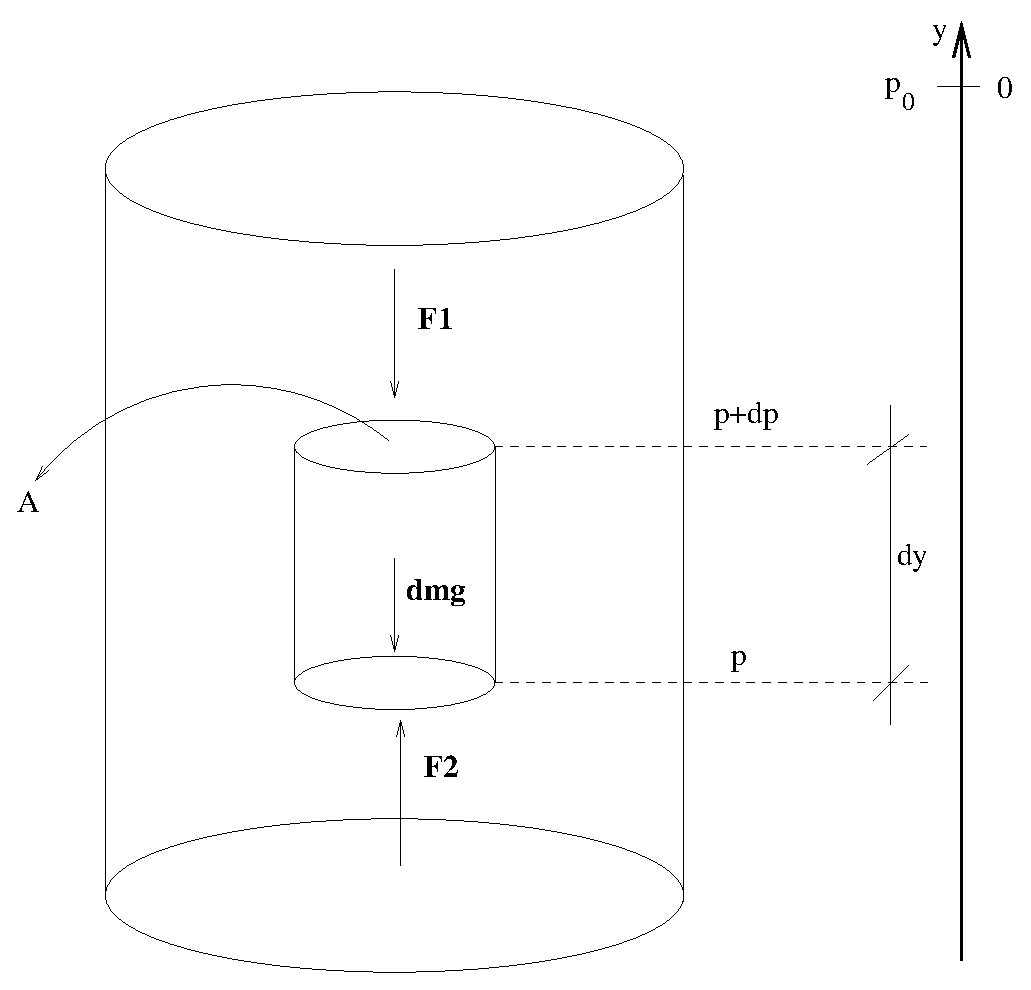
\includegraphics[scale=0.4]{immagini/fisica1/legge_di_stevino1}
\end{figure}


Il fluido è in equilibrio quindi $\ve F_1+\ve F_2+\ud m\ve g=0$. $\ve F_1$ è la forza dovuta alla pressione della parte superiore del fluido, $\ve F_2$ a quella inferiore.
\[-\ud mg-(p+\ud p)A+pA=0\qquad -\ud mg-dpA=0\]
\[\ud m=\rho \ud V=\rho A\ud y\qquad -\rho A\ud y g-\ud p A=0\]
\[\ud p=-\rho g \ud y\]
\[p_0=\text{pressione atmosferica}\]
\[\text{Integrando: }\int_{p_0}^p \ud p=-\int_0^y \rho g\,\ud y=-\rho g\int_0^h\!\ud y\]
\[p=p_0-\rho g y = p_0+\rho g h\]
che è la legge di Stevino e $h$ è la profondita, valida se consideriamo la densità costante, come per esempio in un liquido, per un gas ciò non è più possibile quindi ipotizzando che \[\frac{\rho}{\rho_0}=\frac{p}{p_0}\quad\Rightarrow\quad \rho=\rho_0\frac{p}{p_0}\]
\[\ud p=-\rho_0\frac{p}{p_0}g\ud y\qquad \int_{p_0}^p \frac{\ud p}{p}=\int_0^y -\rho_0\frac{g}{p_0}\ud y\]
\[\log p-\log p_0=\log\frac{p}{p_0}=-\rho_0\frac{g}{p_0}y\]
\begin{equation}
p=p_0e^{-\frac{\rho_0 g}{p_0}y}
\label{legge_atmosfera}
\end{equation}
\[p=p_0e^{-\frac{y}{\lambda}}\qquad \lambda=\frac{p_0}{\rho_0 g}\quad \text{è una lunghezza}\]
che è la legge dell'atmosfera.

\subsection{\index{legge!dei vasi comunicanti}Legge dei vasi comunicanti}
Nel tubo a U (fig.\@\ref{vasicom}) sono introdotti due liquidi non miscibili 1 e 2. Sotto ad A e B c'è solo il fluido 2. A e B sono alla stessa altezza, quindi per la legge di Stevino devono avere la stessa pressione infatti il punto inferiore del tubo ad U avrà una certa pressione $P_{\max}$, la pressione nel punto $A$ sarà $P_{\max} - \rho_a g h_{OA}$ e nel punto $B$ $P_{\max} - \rho_a g h_{OB}$, ma $h_{OA}=h_{OB}$. Usando ancora la legge di Stevino:
\begin{figure}[htbp]
\centering
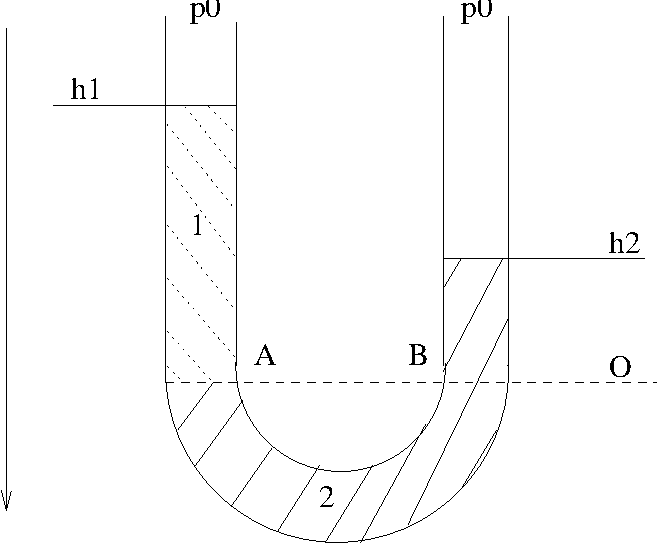
\includegraphics[scale=0.5]{immagini/fisica1/vasi_comunicanti}
\caption{Vasi comunicanti.}
\label{vasicom}
\end{figure}
\[p_A=p_B\qquad p_0+\rho_1 gh_1=p_0+\rho_2gh_2\]
\[\text{legge dei vasi comunicanti: }\frac{\rho_1}{\rho_2}=\frac{h_2}{h_1}\]
in particolare se $\rho_1=\rho_2$ allora $h_1=h_2$.
\subsection{Esperimento di \index{Torricelli}\index{esperimento!di Torricelli}Torricelli}
L'esperimento del 1664 (fig.\@\ref{estor}) consiste nel riempire fino all'orlo un cilindro di mercurio e di rovesciarlo, senza far uscire il liquido, in una bacinella in cui c'è già del mercurio. Il livello del mercurio scende nel cilindro fino al livello di \si{0.76}{\meter}.
\begin{figure}[htbp]
\centering
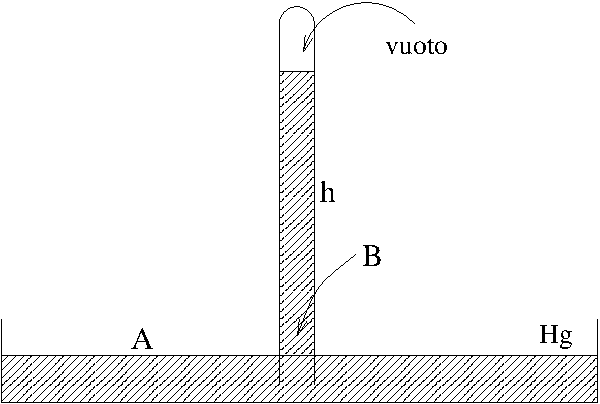
\includegraphics[scale=0.7]{immagini/fisica1/Torricelli}
\caption{Esperimento di Torricelli.}
\label{estor}
\end{figure}

Il punto A e il punto B sono allo stesso livello, quindi: $p_A=p_B$
\[p_A=p_0\qquad p_B=\rho_{\mathrm{Hg}}gh\qquad p_0=\rho_\mathrm{Hg}gh=\si{1}{\atmosphere} \]
Si misura in questo modo la pressione atmosferica, in $\mmHg$.\index{pressione! atmosferica}

L'esperimento di Torricelli suscitò clamore perché Torricelli suppose che nella zona superiore del tubo ci ``fosse'' del vuoto.\index{vuoto}

\subsection{Esperimento delle due semisfere\index{esperimento!delle due semisfere}}
In due semisfere attaccate in modo da creare una sfera unica viene diminuita la pressione togliendo aria. In questo modo la pressione esterna è maggiore ed esercita una forza sulle pareti delle semisfere, rendendo difficile la separazione.
\begin{figure}[htbp]
\centering
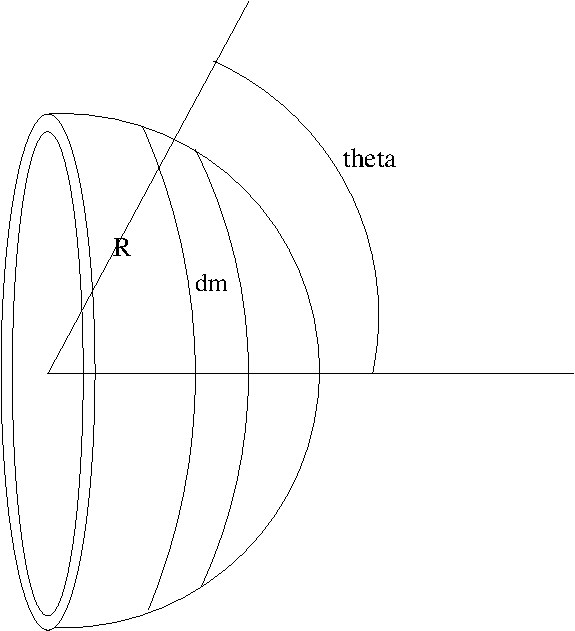
\includegraphics[scale=0.5]{immagini/fisica1/Sfera_pressione}
\end{figure}

Consideriamo la strisciolina $\ud m$
\[F=\int\ud F\]
\[\ud A=2\pi R\sin\theta R\ud\theta=2\pi R^2\sin\theta\ud\theta\]
\[\ud F_x=p_0 \ud A\cos\theta\]
\[\frac{\ud \sin\theta}{\ud \theta}=\cos\theta\qquad\ud\sin\theta=\cos\theta\ud\theta\]
\[\int_S \ud F_x=p_0 2\pi R^2\int_0^{\frac{\pi}{2}}\sin\theta\cos\theta\ud\theta=p_0 2\pi R^2\int_0^{1}\sin\theta\ud(\sin\theta)=p_0\pi R^2\]
\[\text{se } R=\SI{1}{\metre} \quad F_x\simeq\SI{3E5}{\newton} \]

\subsection{Principio di Pascal\index{principio!di Pascal}}
\begin{Pri}[Pascal]
 La variazione di pressione dovuta a forze esterne si trasmette invariata in tutti i punti del fluido.
\end{Pri}

Consideriamo un cilindro con un pistone che non esercita pressione.

\begin{figure}[htbp]
\centering
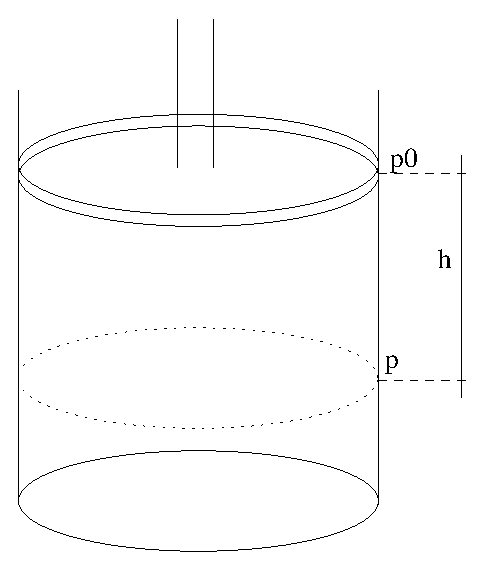
\includegraphics[scale=0.5]{immagini/fisica1/Pascal1}
\end{figure}

Se applichiamo una forza sul pistone la pressione esterna, al livello del pistone, salirà da $p_0$ a $p_0+p_0'$
\begin{align*}
\text{Prima:}&\quad p=p_0+\rho gh\\
\text{Dopo:}&\quad p=p_0+p_0'+\rho gh=p+p_0'
\end{align*}
cioè la variazione di pressione si trasmette in tutti i punti del fluido.
\subsubsection{Paradosso di Pascal}
Pascal si divertiva a rompere le botti infilandogli un tubo molto lungo, anche di sezione sottile, in quanto la sezione non conta, pieno d'acqua. La pressione faceva rompere le botti.

\subsection{Principio di Archimede\index{principio!di Archimede}}
Consideriamo un elemento di un fluido. Su di esso agisce la forza peso, perché sia in equilibrio deve agire una forza uguale e contraria: la spinta di Archimede $\ve S=-\rho V\ve g$. Essa è dovuta alla differenza di pressione $\Delta p$. Se sostituiamo l'elemento di fluido con un solido il contorno non cambia e quindi la spinta di Archimede risulta uguale. Il peso però è cambiato, quindi in generale non è in equilibrio, infatti la somma delle forze:
\[
 \rho V\ve g - \rho_\text{fluido}V\ve g \neq 0
\]
Se $P>S$ cioè $\rho>\rho_\text{fluido}$ sprofonda, altrimenti il corpo sale e bisogna considerare che una parte di questo emergerà e allora la spinta di Archimede diminuirà. La condizione di equilibri in questo caso è:
\[
 \rho V\ve g - \rho_\text{fludio}V_\text{immerso}\ve g = 0
\]
la soluzione è $V_\text{immerso}=\frac{\rho}{\rho_\text{fluido}}V$ e poiché è sicuramente vero che $V_\text{immerso}\leq V$ allora deve essere $\rho\leq\rho_\text{fluido}$.


\begin{Es}[Iceberg]
\marginpar{
\begin{tiny}ecco quello che dicono i nostri matematici\end{tiny}
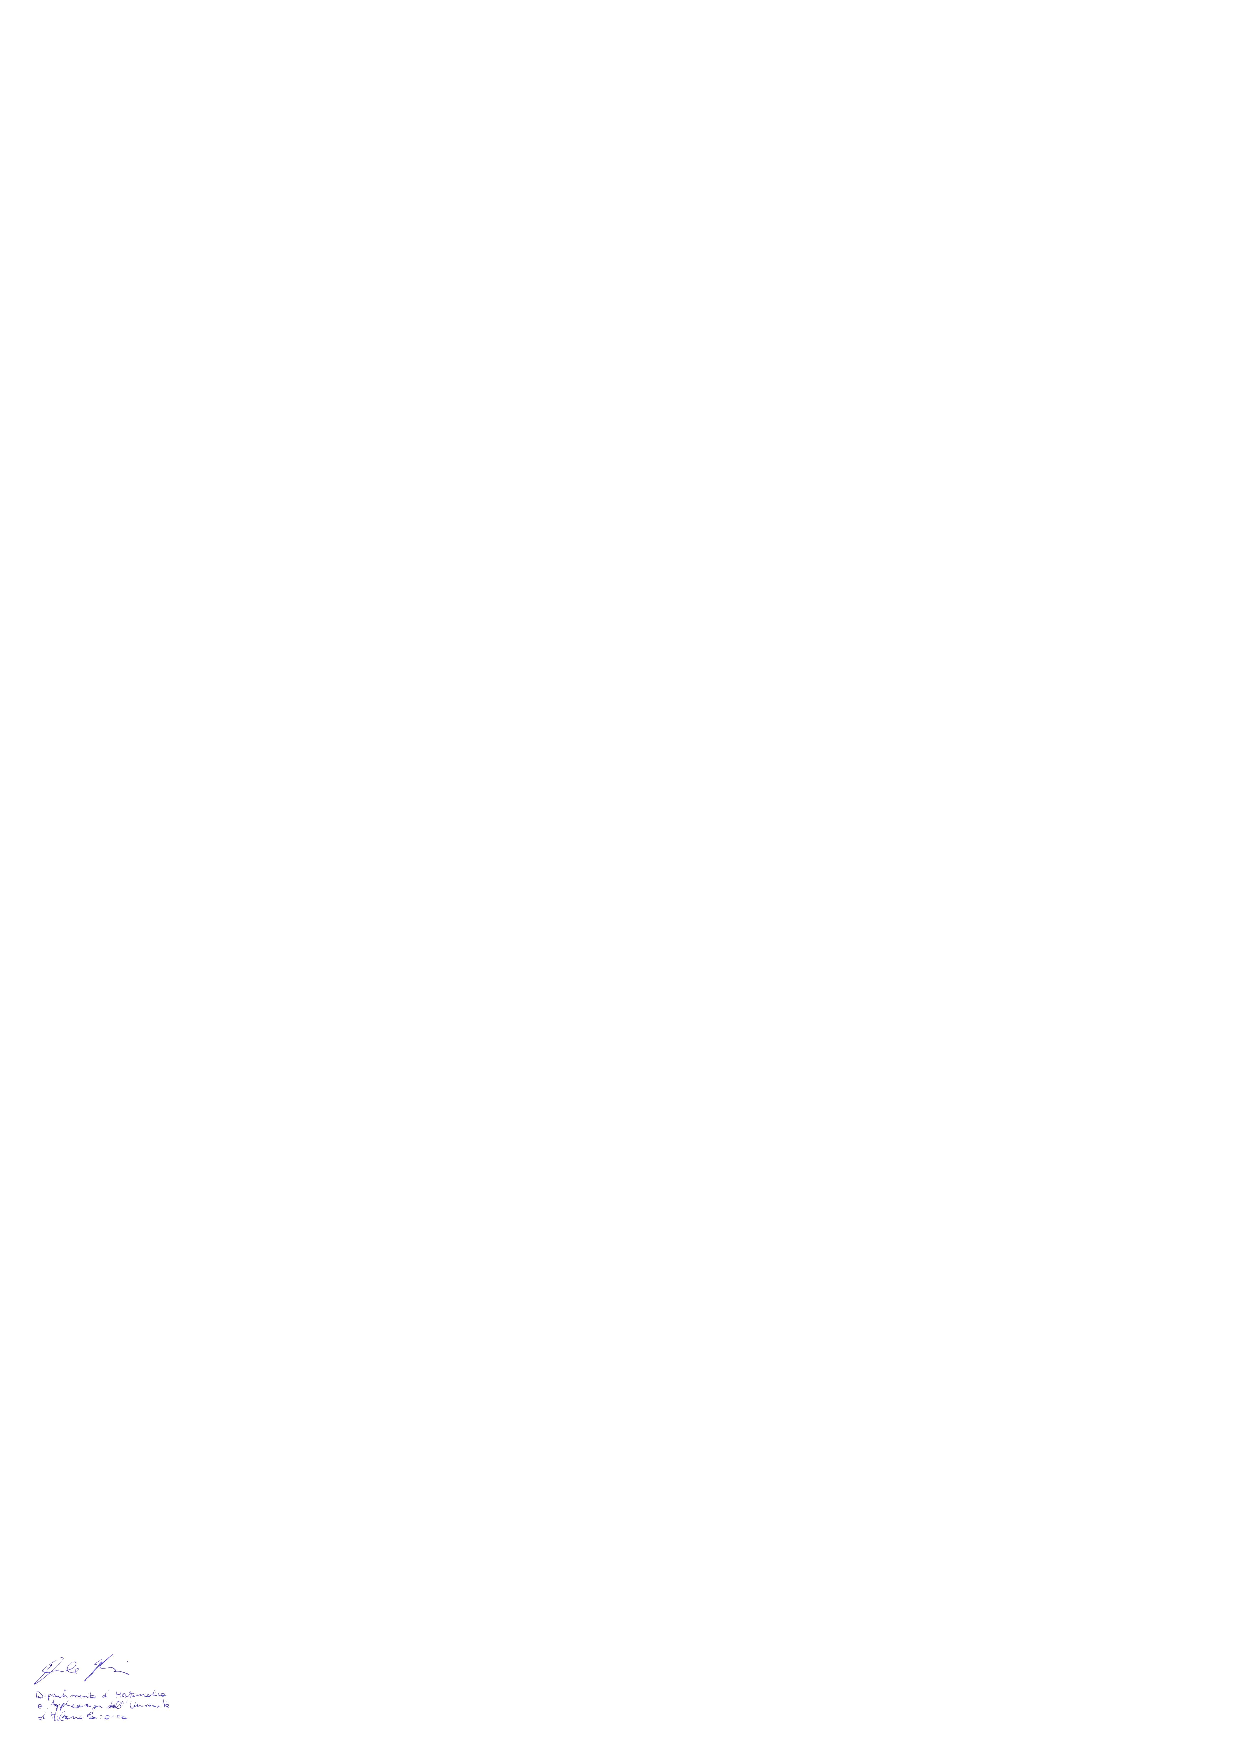
\includegraphics[scale=1.4]{immagini/fisica1/firma_daniele}
}
Ghiaccio in acqua $\Longrightarrow$ si scioglie
\[V_\text{totale}-V_\text{emergente}=V_\text{totale}\frac{\rho_\text{ghiaccio}}{\rho_\text{\ce{H2O}}}\]
\[V_\text{totale}\simeq 10 V_\text{emergente}\]
\end{Es}
\subsection{Condizione generale di equilibrio}
\begin{figure}[htbp]
   \centering
   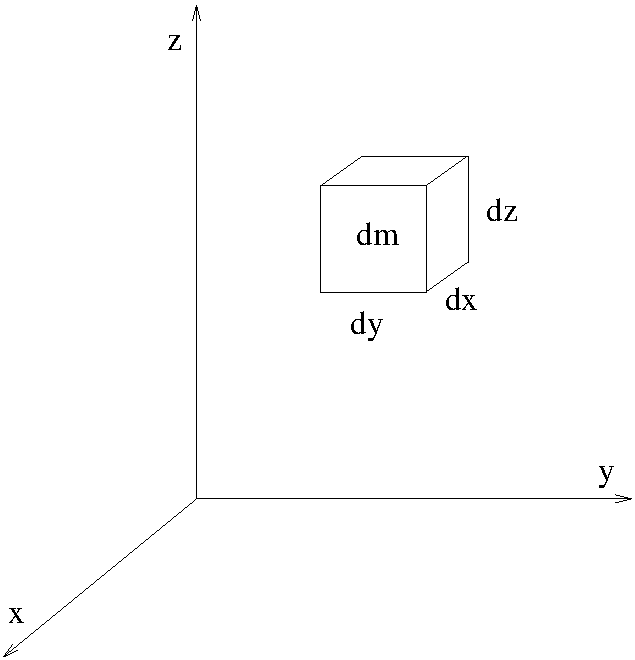
\includegraphics[scale=0.4]{immagini/fisica1/equilibrio}
\end{figure}
Forze di volume: proporzionali al volume
\[\ve f=\frac{\ve F}{m}\]
notare che $\ve f$ è un'accelerazione.


Forze di superficie: dovute al liquido che lo circonda, proporzionali alla superficie
\[F=pA\]
Lungo l'asse $x$:

\[f_x\ud m+p(x)\ud z\ud y-p(x+\ud x)\ud y\ud z=0\]
\[f_x\rho\ud x\ud y\ud z+p(x)\ud y\ud z-(p(x)+\frac{\partial p}{\partial x}\ud x)\ud y\ud z=0\]
\[f_x\rho\ud x\ud y\ud z-\frac{\partial p}{\partial {x}}\ud x\ud y\ud z=0\]
\[f_x\rho=\frac{\partial p}{\partial x}\quad f_y\rho=\frac{\partial p}{\partial y}\quad f_z\rho=\frac{\partial p}{\partial z}\]
\begin{equation}\ve f\rho=\ve\nabla p\end{equation}

\begin{Es}[Forza peso -- Stevino]
Nelle ipotesi di Stevino c'è solo il peso, quindi $\ve f=\ve g$
\[
f_z\rho=\frac{\ud p_z}{\ud z}\quad g\rho\ud z=\ud p \quad p=p_0+\rho gz
\]
In generale:
\[U_m=\frac{U}{m}\qquad \rho\ve f=-\rho\ve\nabla(U_m)=\ve\nabla p\qquad -\ve\nabla(\rho U_m)=\ve\nabla p\]
\[\rho U_m=-p+\const\]
Segue che le superficie isobariche \index{superficie!isobarica}coincidono con le superfici equipotenziali. Nel caso agisca solo la forza peso esse sono dei piani orizzontali: $U_m = -gz+U_0$.
\end{Es}
\begin{Es}[Fluido in accelerazione]
 \begin{figure}[htbp]
 \centering
 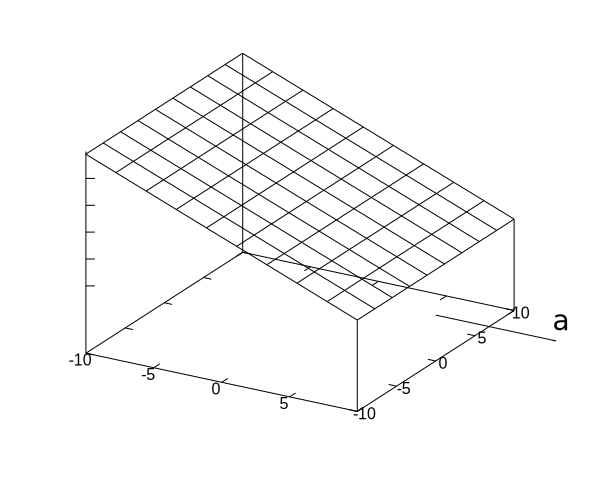
\includegraphics[scale=0.5]{immagini/fisica1/fluido_accelerato}
 % fluido_accelerato.pdf: 480x384 pixel, 72dpi, 16.93x13.55 cm, bb=0 0 480 384
\end{figure}
 Se un fluido è accelerato verso destra con accelerazione $a$ allora usando le forze fittizie: $\ve F=m\ve g-m\ve a$:
\[
 \ve f = -g\ver j - a \ver i
\]
l'equazione differenziale risultante:
\[
 \begin{cases}
  -a\rho=\frac{\partial p}{\partial x}\\
  -g\rho=\frac{\partial p}{\partial y}
 \end{cases}
\]
la cui soluzione è:
\[
 p = \rho(-ax-gy)
\]
e le superfici isobariche (ed equipotenziali):
\[
 y = -\frac{p}{\rho g} - \frac{a}{g}x
\]
che è un piano la cui pendenza è proporzionale all'accelerazione del sistema.
\end{Es}
\begin{Es}[Fluido in rotazione\index{moto!circolare!di un fluido}]
\begin{figure}[htbp]
\centering
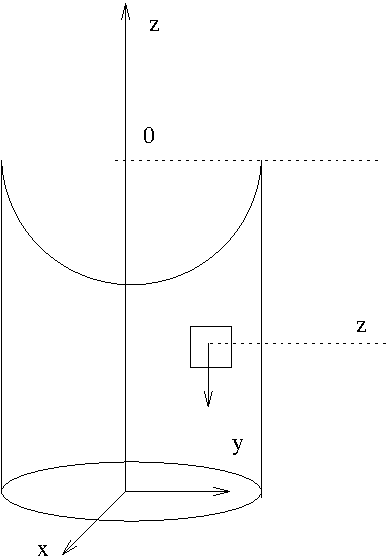
\includegraphics[scale=0.65]{immagini/fisica1/fluido_rotazione}
\caption{Elemento di un fluido in rotazione.}
\end{figure}
Per lavorare in un sistema non inerziale ed usare la legge di Newton aggiungiamo la forza fittizia $m\omega^2 r$, $r$ è la distanza dal centro, la distanza dell'elemento $\ud m$ dall'asse.
\[\text{Nella direzione radiale } f_r=\omega^2 r\]
\[f_r\rho=\rho\omega^2 y=\frac{\ud p}{\ud y}\qquad \ud p=\rho\omega^2 y\ud y\]
\[\int_{p_\text{asse}}^p\ud p=\int_0^R \rho\omega^2 y\ud y\]
\[p-p_\text{asse}=\rho\omega^2\frac{R^2}{2}\qquad p=p_\text{asse}+\frac{\rho\omega^2}{2}R^2\]
\[p_\text{asse}=p_0-\rho gz\qquad p=p_0-\rho gz+\frac{\rho\omega^2}{2}R^2\]
Su una superficie isobarica $p=\const$,
\[\rho gz=\const+\frac{\rho\omega^2}{2}R^2\]
\[z=\const+\frac{\rho\omega^2}{2\rho g}R^2=\const+\frac{\omega^2}{2g}R^2=\const+\frac{\omega^2}{2g}(x^2+y^2)\]
\`E un paraboloide:
\begin{figure}[htbp]
\centering
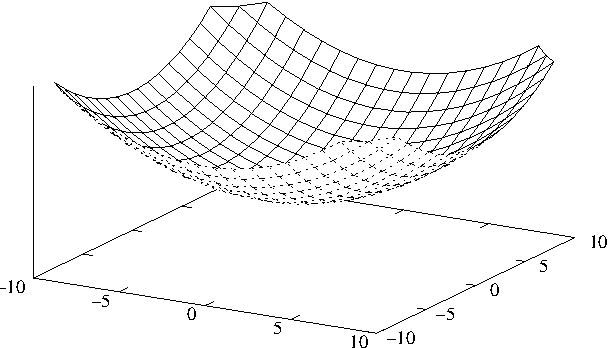
\includegraphics[scale=1]{immagini/fisica1/paraboloide}
\caption{Paraboloide.}
\end{figure}
\subsubsection{Archimede per le rotazioni}
Come per il caso in cui c'è solo la forza di gravità anche nel caso di fluido in rotazione vale lo stesso risultato, cioè che se l'oggetto è meno denso del fluido si sposta verso l'esterno se più denso verso l'interno. Infatti consideriamo solo la forza centrifuga (oppure il limite per $\omega$ molto alto) allora la spinta di archimede verso l'interno sarà: $\rho_\text{fluido}V\omega^2 r$. Allora la somma delle forze verso l'esterno sarà:
\[
 \rho V\omega^2 r-\rho_\text{fluido}V\omega^2 r
\]
quindi a meno che $r=0$ il corpo si muove verso l'esterno se $\rho>\rho_\text{fluido}$. Questo è il principio delle centrifughe.
\end{Es}

\section{Dinamica dei fluidi\index{dinamica!dei fluidi}}
\begin{description}
\item[Approccio di Lagrange\index{Lagrange}]: si danno le coordinate $x$ di un elemento di flusso in funzione del tempo, è un metodo di analisi complicato.
\item[Approccio di Eulero\index{Eulero}]: si studiano le caratteristiche del fluido in un determinato punto. Ci mettiamo in un punto dello spazio e vediamo come variano le grandezze in funzione del tempo. Per descrivere in modo completo bisogna ripetere le misurazioni in modo completo.
\end{description}
Vengono usate le semplificazioni:
\begin{itemize}
\item fluidi:
\begin{itemize}
\item incomprimibili ($\rho=\const$)
\item non viscosi (primi di attrito interno)
\end{itemize}
\item moto:
\begin{itemize}
\item stazionario (i fenomeni non dipendono dal tempo)
\item irrotazionale (nessun vortice, non caotici), $\mathrm{rot}(\ve v)=0$, $\oint \ve v \ud \ve s=0$
\end{itemize}
\end{itemize}
\begin{description}
 \item [Linee di flusso\index{linee!di flusso}]: linee tangenti alla $\ve v$ della particella. Ha senso se il moto è stazionario, cioè se $\ve v$ è costante nel tempo. 
 \item[Tubo di flusso] Le linee di flusso danno origine al tubo di flusso\index{tubo!di flusso}. Non è possibile che vi sia fuoriuscita di fluido latente per definizione: $\ve v$ è tangente alle linee di flusso.
\end{description}

\subsection{Equazione di continuità\index{equazione!di continuità}}
La portata volumica è la quantità di volume che passa nel tempo: $Q=\frac{\ud V}{\ud t}$, ma essendo in regime stazionario la velocità non varia, quindi $Q=\frac{\Delta V}{\Delta t}$, la portata di massa è la quantità di massa nel tempo.

\begin{figure}[htbp]
\centering
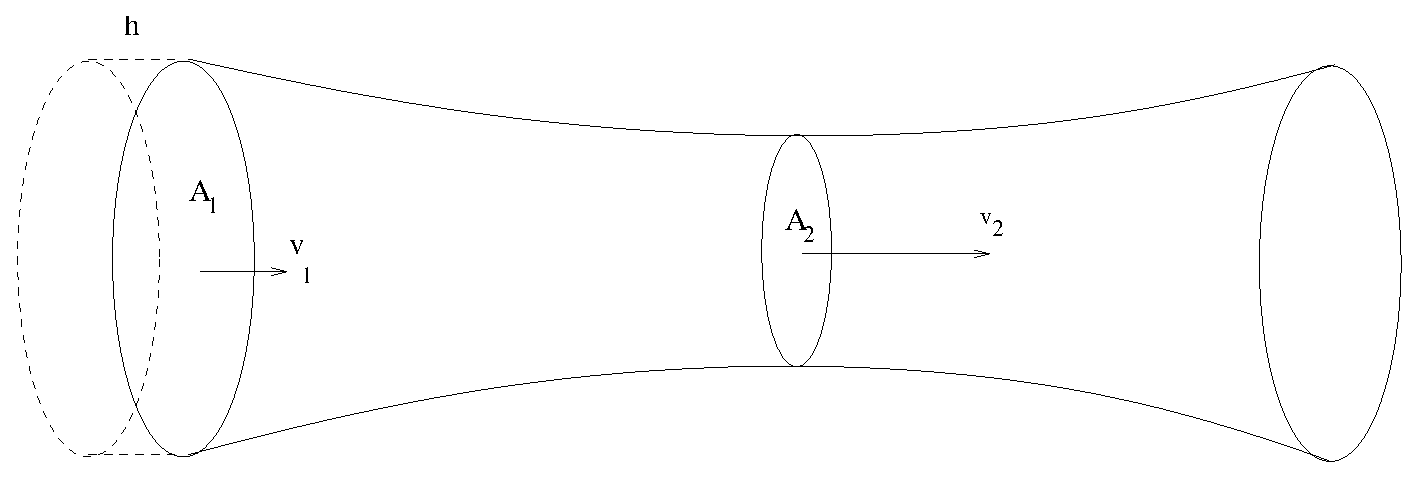
\includegraphics[scale=0.4]{immagini/fisica1/equazione_continuita}
\end{figure}
Fissiamo $\Delta t$ tale che $h=v_1\Delta t$
\begin{enumerate}
\item fluido che entra in $\Delta t\quad \rho\Delta V=\rho A_1v_1\Delta t$
\item fluido che esce in $\Delta t\quad \rho\Delta V=\rho A_2v_2\Delta t$
\end{enumerate}
Naturalmente le masse entranti e uscenti sono uguali, quindi (legge di Leonardo\index{legge!di Leonardo}\index{Leonardo}):
\[A_1v_1=A_2v_2\]

Portata volumica\index{portata!volumica}: $Q_v=Av$

Portata di massa\index{portata!di massa}: $Q_m=\rho Av$

\subsection{Equazione di Bernoulli\index{equazione!di Bernoulli}}


\begin{center}
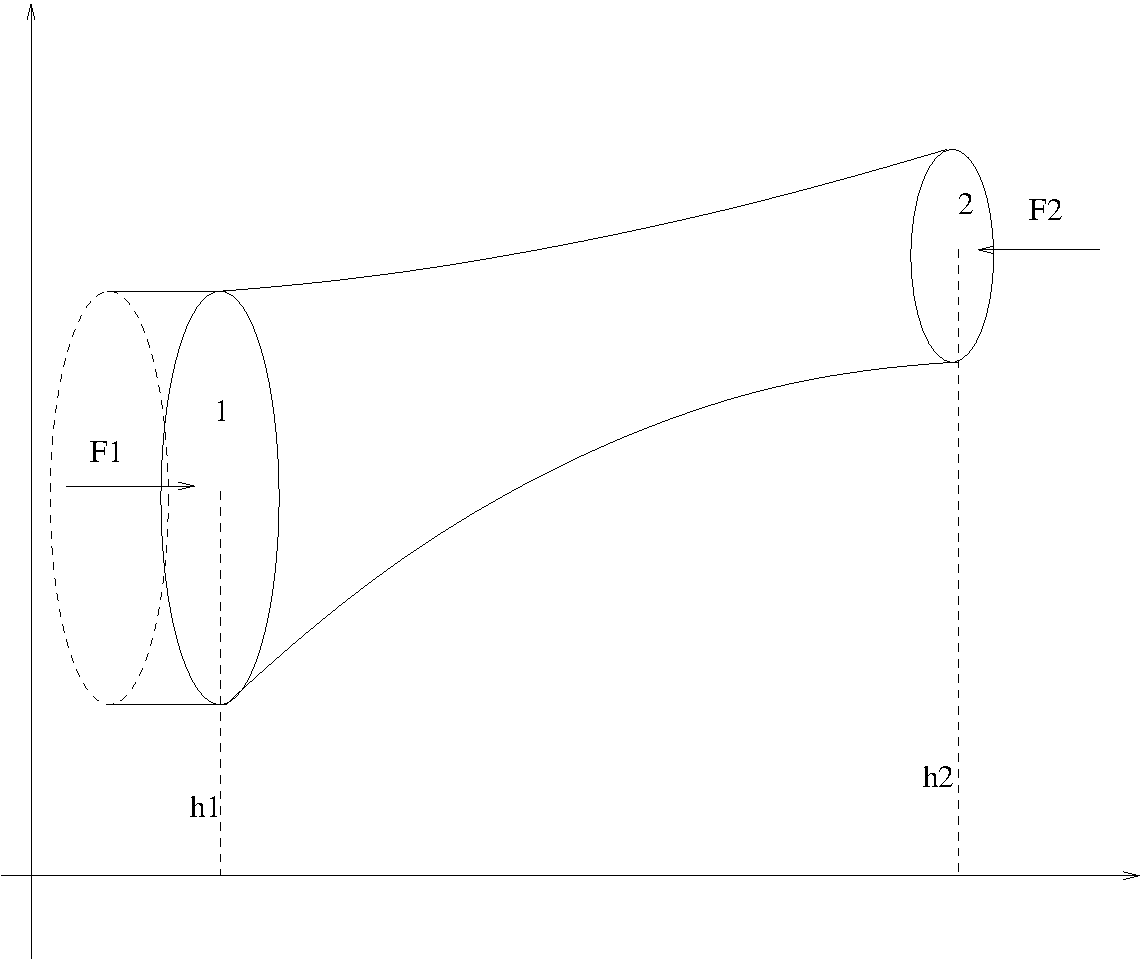
\includegraphics[scale=0.4]{immagini/fisica1/Bernoulli}
\end{center}
Consideriamo un tempo $\Delta t$ piccolo e una porzione di massa $\Delta m$. L'effetto netto tra la situazione iniziale e quella finale è di spostare l'elementino da un'estremità all'altro.

Il lavoro è svolto dalla forze esterne: $\ve F_1, \ve F_2, \ve P$ è $L=\Delta K$ poiché non c'è variazione di energia potenziale.
\[\Delta m=\rho \Delta V=\rho A_1 v_1\Delta t=\rho A_2 v_2 \Delta t\]
\[
\left\{
        \begin{array}{lll}
        L_1=F_1\Delta S_1=F_1v_1\Delta t=p_1A_1v_1\Delta t\\
        L_2=-F_2\Delta S_2=-F_2v_2\Delta t=-p_2A_2v_2\Delta t\\
        L_P=-\Delta mg(h_2-h_1)
        \end{array}
\right.
\]
\[\Delta K=\frac{1}{2}\Delta m(v_2^2-v_1^2)\]
\[L_1+L_2+L_P=\Delta K\]
\[p_1A_1v_1\Delta t-p_2A_2v_2\Delta t-\Delta mg(h_2-h_1)=\frac{1}{2}\Delta m(v_2^2-v_1^2)\]
\begin{align*}
&\Delta m\left[\left(gh_1-gh_2\right)+\frac{p_1A_1v_1\Delta t}{\Delta m}-\frac{p_2A_2v_2\Delta t}{\Delta m}\right]\\
=&\Delta m\left[\left(gh_1-gh_2\right)+\frac{p_1A_1v_1\Delta t}{\rho A_1v_1\Delta t}-\frac{p_2A_2v_2\Delta t}{\rho A_2v_2\Delta t}\right]\\
=&\Delta m\left[gh_1-gh_2+\frac{p_1}{\rho}-\frac{p_2}{\rho}\right]=L\\
=&\Delta K=\frac{1}{2}\Delta m(v_2^2-v_1^2)
\end{align*}
\[gh_1-gh_2+\frac{p_1}{\rho}-\frac{p_2}{\rho}=\frac{1}{2}(v_2^2-v_1^2)\]
\[gh_1+\frac{p_1}{\rho}+\frac{1}{2}v_1^2=gh_2+\frac{p_2}{\rho}+\frac{1}{2}v_2^2\]
\begin{Teo}[Bernoulli]
 Per un flusso laminare, incomprimibile, non viscoso e irrotazionale vale:
 \begin{equation}
  \rho gh+p+\frac{1}{2}\rho v^2=\const
\end{equation}
\end{Teo}
Nel caso che $v=0$ l'unico termine che sopravvive è quello che è chiamato \index{pressione!statica}pressione statica: $p+\rho gh$ in quanto è presente anche quando il fluido è fermo. L'altro termine invece è presente da solo se il fluido scorre in orizzonatale, quindi $\frac{1}{2}\rho v^2$ è detta \index{pressione!dinamica}pressione dinamica. In questo caso:
\[
 p_1+\frac{1}{2}\rho v_1^2=p_2+\frac{1}{2}\rho v_2^2=\const
\]
quindi si deduce che se la velocità è piccola la pressione è grande. Questo può essere spiegato anche usando l'equazione di continuità, infatti dove il tubo è più stretto la velocità è maggiore, questo significa che ci è stata un'accelerazione e quindi una forza dovuta ad una variazione di pressione che deve essere maggiore dove il tubo è più largo.

L'espressione del teorema di Bernoulli è molto simile alla conservazione dell'energia meccanica.
\[mgh+\frac{1}{2}mv^2=\const\]
\begin{Es}[ali di aereo]
L'aria sotto le ali di un aereo è più lenta di quella che passa sopra, quindi dalla legge di Bernoulli, considerando l'altezza uguale:
\[p_\text{sopra}+\frac{1}{2}\rho v_\text{sopra}^2=p_\text{sotto}+\frac{1}{2}\rho v_\text{sotto}^2\]
quindi se $v_\text{sopra}>v_\text{sotto}$ allora $p_\text{sopra}<p_\text{sotto}$ e allora c'è una forza netta verso l'alto.

Un altro contributo viene dal fatto che l'aria è fatta deviare verso il basso e il per terzo principio della dinamica ci deve essere una forza uguale e contrario applicata sulle ali. Tutto questo contribuisce alla \index{portanza}portanza.
\end{Es}
\section{Viscosità\index{viscosità}\index{eta@$\eta$|see{viscosità}}}
\label{viscosita fisica1}
\begin{figure}[htbp]
\centering
\subfigure{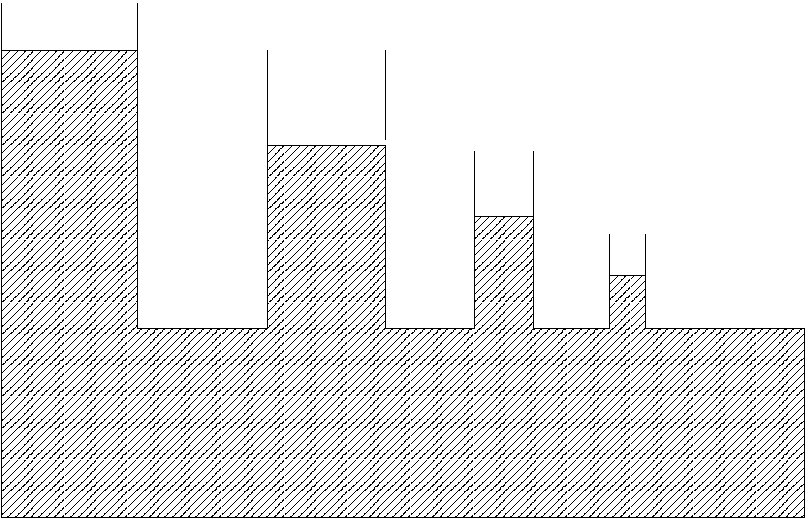
\includegraphics[scale=0.45]{immagini/fisica1/viscosita1}}\quad
\subfigure{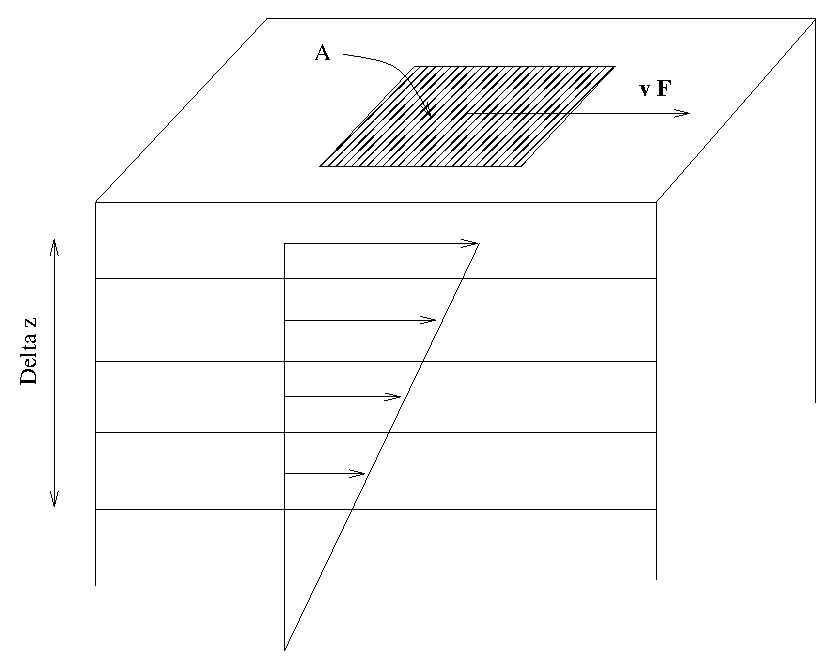
\includegraphics[scale=0.4]{immagini/fisica1/viscosita2}}
\caption{Perdita di pressione a causa della viscosità.}
\end{figure}

La pressione diminuisce, si ha una perdita di carico per un fluido viscoso a causa degli attriti interni. Siamo a regime laminare (velocità basse).


\[F=\eta A\frac{\ud v}{\ud z}\qquad\ve F=\eta A \ve\nabla v\qquad\eta=\text{coefficiente di viscosità}\]

\subsection{Legge di Poiseuille}

\vspace{0.4cm}
\begin{center}
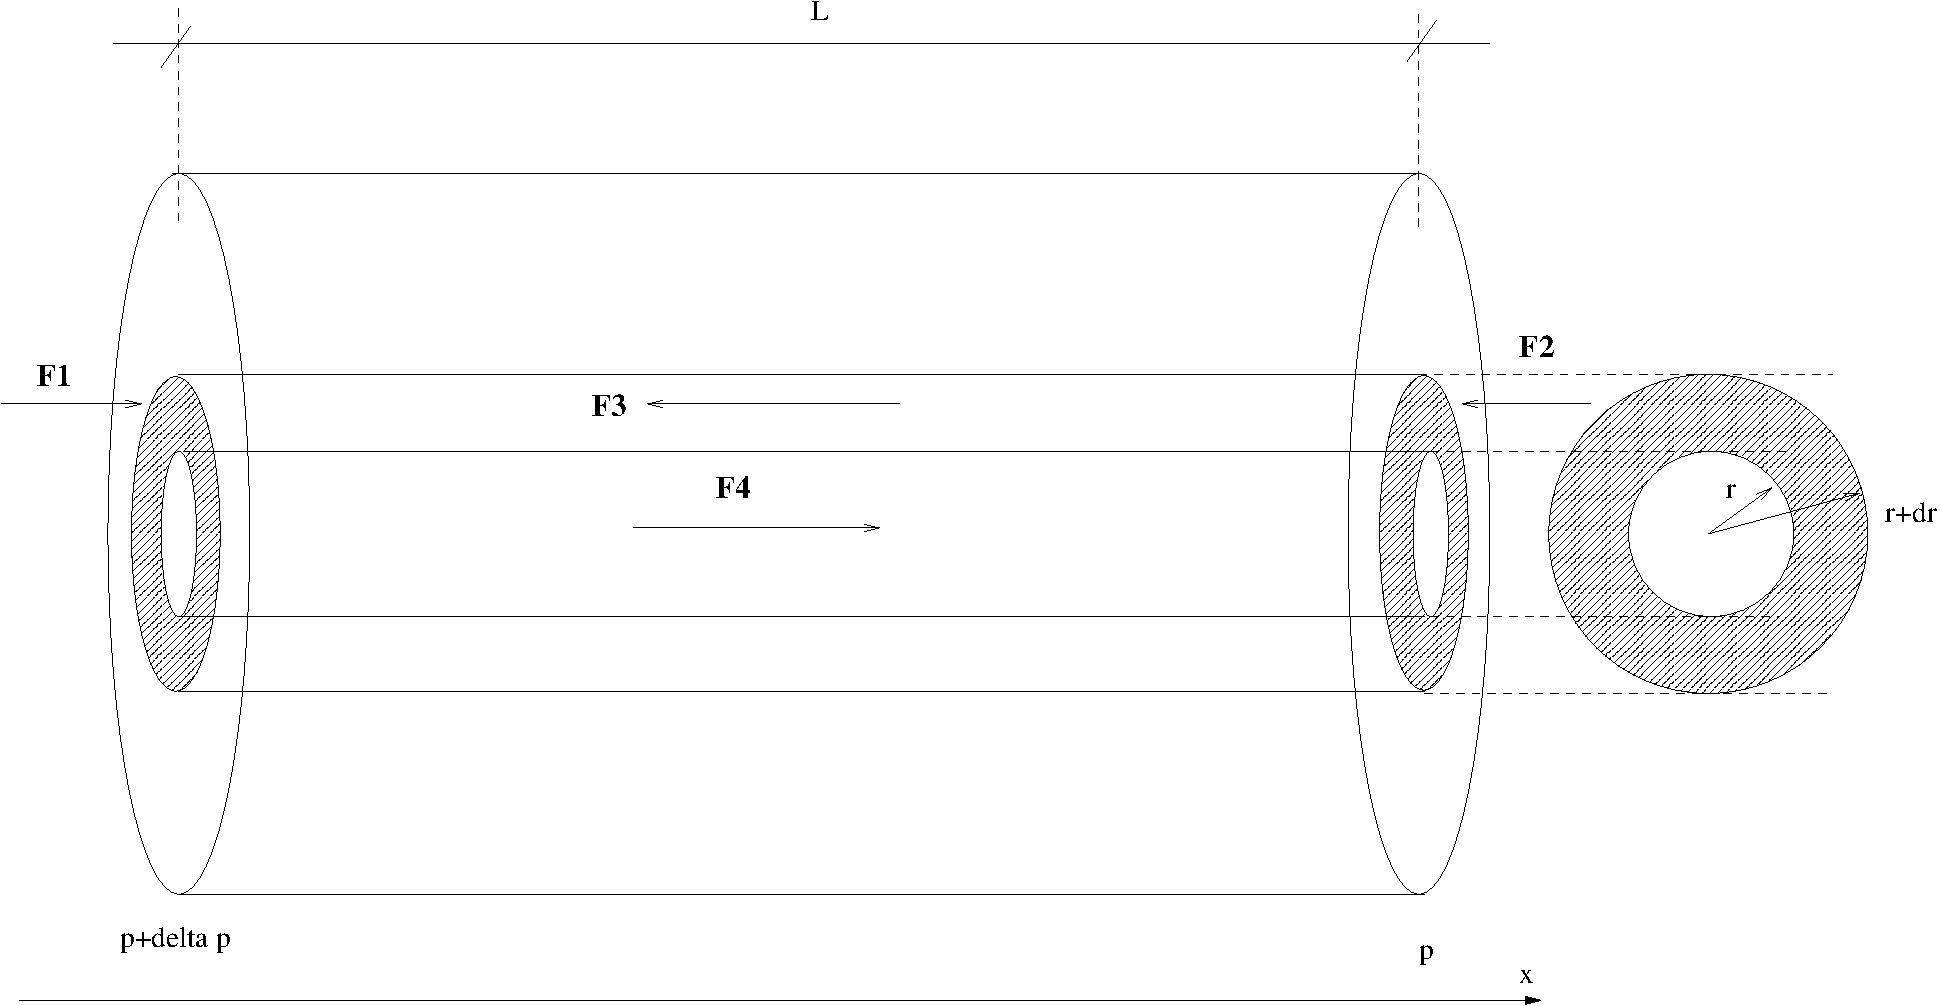
\includegraphics[scale=0.4]{immagini/fisica1/Poiseuille}
\end{center}


La velocità sarà massima al centro e minima ai bordi. Considero la porzione di fluido tra $r$ e $r+\ud r$. Le forze $F_3$ e $F_4$ sono dovute alle porzioni di fluido più esterne (più lente) e quelle più interne (più veloci).
\[F_1=(p+\Delta p)2\pi r\ud r\qquad F_2=-p2\pi r\ud r\]
\[F_3=L2\pi (r+\ud r)\eta\left. \frac{\ud v}{\ud r}\right|_{r+\ud r}\quad \frac{\ud v}{\ud r}<0\]
\[F_4=-L2\pi r\eta\left.\frac{\ud v}{\ud r}\right|_r\]
\[0=\sum F=(p+\Delta p)2\pi r\ud r-p 2\pi r\ud r+L 2\pi (r+\ud r)\eta\left.\frac{\ud v}{\ud r}\right|_{r+\ud r}\!\!\!\!\!\!\!\!\!\!-L2\pi r\eta\left.\frac{\ud v}{\ud r}\right|_r\]
\[\text{Taylor nell'intorno di $x=r$:\quad} \left.\frac{\ud v}{\ud r}\right|_x=\left.\frac{\ud v}{\ud r}\right|_r+\left.\frac{\ud^2 v}{\ud r^2}\right|_r(x-r)+\ldots\]


\[0=\Delta p r\ud r+\eta L\left\{(r+\ud r)\left.\frac{\ud v}{\ud r}\right|_{r+\ud r}\!\!\!\!\!\!\!\!\!\!-r\left.\frac{\ud v}{\ud r}\right|_r\right\}\simeq\]
\[\simeq\Delta p r\ud r+\eta L\left\{(r+\ud r)\left[\left.\frac{\ud v}{\ud r}\right|_r+\left.\frac{\ud^2 v}{\ud r^2}\right|_r\ud r\right]-r\left.\frac{\ud v}{\ud r}\right|_r\right\}=\]
\[=\Delta p r\ud r+\eta L\left\{r\frac{\ud v}{\ud r}+r\frac{\ud^2 v}{\ud r^2}\ud r+\ud r\frac{\ud v}{\ud r}+\frac{\ud^2 v}{\ud r^2}\ud r^2-r\frac{\ud v}{\ud r}\right\}\simeq\]
\[\simeq\Delta p r \ud r+\eta L\left[r\frac{\ud^2 v}{\ud r^2}\ud r+\frac{\ud v}{\ud r}\ud r\right]=0\]
\[\Delta p r+\eta L\left[r\frac{d^2 v}{\ud r^2}+\frac{\ud v}{\ud r}\right]=0\]
\[r\Delta p+\eta L\frac{\ud}{\ud r}\left(r \frac{\ud v}{\ud r}\right)=0\]
\[r\Delta p=-\eta L\frac{\ud}{\ud r}\left(r\frac{\ud v}{\ud r}\right)\]
\[\int_0^r r'\Delta p\,\ud r'=-\eta L\int_0^r\frac{\ud}{\ud r'}\left(r'\frac{\ud v}{\ud r'}\right)\ud r'\]
\[\Delta p\frac{1}{2}r^2=-\eta L r\frac{\ud v}{\ud r}\]
\[\Delta p\frac{1}{2}r=-\eta L \frac{\ud v}{\ud r}\]
\[\frac{\Delta p}{2}\int_R^r r'\,\ud r'=-\eta L\int_0^v \ud v'\]
\[\frac{\Delta p}{4}\left[r^2-R^2\right]=-\eta Lv\]
\[v=-\frac{\Delta p}{4}\frac{r^2-R^2}{\eta L}=\frac{\Delta p}{4\eta L}\left(R^2-r^2\right)\]
\begin{align*}
Q_v&=\int v \,\ud A=\int_0^R v(r)2\pi r\,\ud r=\int_0^R\frac{2\pi r\Delta p}{4\eta L}(R^2-r^2)\,\ud r\\
&=\frac{1}{2}\pi\int_0^R\frac{r\Delta p}{\eta L}\left(R^2-r^2\right)\ud r\\
&=\frac{\pi}{2}\frac{\Delta p}{\eta L}\int_0^R \left(rR^2-r^3\right)\ud r=\frac{\pi}{2}\frac{\Delta p}{\eta L}\left(\frac{R^4}{2}-\frac{R^4}{4}\right)\\
&=\frac{\pi\Delta p}{8\eta L}R^4
\end{align*}
  \begin{legge}[Poiseuille]
  \begin{equation}
    Q_v=\frac{\pi\Delta p}{8\eta L}R^4 
  \end{equation}
\end{legge}
si definisce una resisteza idraulica $\frac{8\eta L R^4}{\pi}$ in analogia con la resistenza elettrica.
\index{meccanica dei fluidi|)}


\chapter{Termodinamica\index{termodinamica|(}}
\minitoc
In meccanica è utile utilizzare ipotesi nelle quali ci siano pochi gradi di libertà, per esempio con i fluidi si usa l'approccio di Eulero. In termodinamica si considerano molte particelle e quindi molti gradi di libertà.

La termodinamica si occupa di scambi di energia e di cambiamento di stato di sistemi macroscopici, descritti da un numero piccolo di variabili macroscopiche come temperatura, volume e pressione. Si tratta sempre di sostanza pure e omogenee (una sola fase).

Una variabile di stato è una variabile\index{variabile!di stato} stazionaria(costante nel tempo), isotropa (uguale in tutte le direzioni), omogenea (uguale nello spazio).

Un sistema\index{sistema} è la porzione di materia sotto osservazione, l'ambiente \index{ambiente} tutto il resto. L'universo termodinamico\index{universo!termodinamico} è l'unione del sistema con l'ambiente. Un sistema aperto \index{sistema!aperto} scambia energia e materia con l'ambiente, un sistema chiuso \index{sistema!chiuso} scambia solo energia, un sistema isolato \index{sistema!isolato}non scambia né energia ne materia. Una parete adiabatica \index{parete!adiabatica}è una parete che non lascia passare calore, una diatermica \index{parete!diatermica}lascia passare calore.

Le variabili di stato vanno considerate dopo un certo tempo di rilassamento del sistema. La termodinamica classica si occupa dei sistemi all'equilibrio, analizza i sistemi prima e dopo le trasformazioni. Le trasformazioni \index{trasformazioni!quasistatiche}vengono considerate quasi statiche, cioè trasformazioni che passano attraverso infiniti stati di equilibrio in un tempo infinitamente lungo. Queste trasformazioni sono dette anche reversibili\index{trasformazioni!reversibili}.

Spesso vengono considerati l'equilibrio meccanico \index{equilibrio!meccanico}(nessun lavoro da e sul sistema), chimico \index{equilibrio!chimico}(nessuna reazione chimica interna), termico \index{equilibrio!termico}(nessuno scambio di calore).

\section{Principio zero della termodinamica\index{principio!zero della termodinamica}}
\begin{figure}[htbp]
\centering
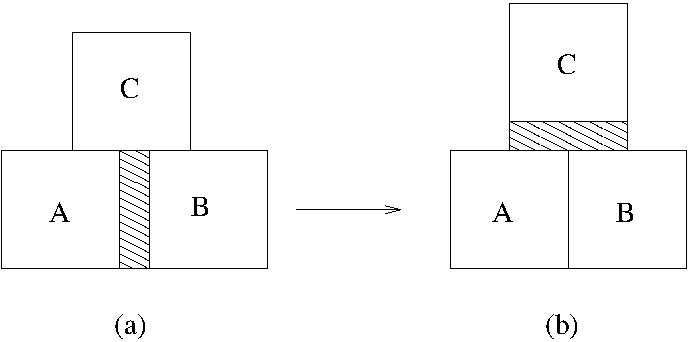
\includegraphics[scale=0.5]{immagini/fisica1/principio_zero}
\caption{(a)A e B scambiano calore con C, raggiungono l'equilibrio. (b) A e B non scambiano calore, sono all'equilibrio.}
\end{figure}
Il principio zero della termodinamica serve per definire il concetto di temperatura:
\begin{Pri}[principio zero della termodinamica]
Se due sistemi sono all'equilibrio termico con un terzo sistema allora sono all'equilibrio termico tra di loro.

Due sistemi hanno la stessa temperatura se sono in equilibrio termico. Due sistemi sono in equilibrio termico se messi a contatto le loro proprietà non cambiano.
\end{Pri}

\section{Temperatura\index{temperatura}}
\index{termometro}Il termometro è lo strumento per la misurazione della temperatura $T$. Per fare un termometro si sceglie una proprietà $X$ che varia in funzione di $T$. Se $X$ varia linearmente in funzione di $T$ allora (in kelvin):
\begin{equation}
T(X)=273.16\frac{X}{X_\text{triplo}}
\end{equation}
$X_\text{triplo}$ è il valore di $X$ al punto triplo dell'acqua ($\si{0.01}{\celsius}$). In questo modo la temperatura del punto triplo dell'acqua è di $\si{273.16}{\kelvin}$. Solitamente $X$ è il volume, la resistenza elettrica, la fem in una termocoppia, la pressione di un gas perfetto a volume costante\ldots I termometri empirici hanno problemi di non linearità e possono essere usati solo in piccoli intervalli dove si ritiene che il problema della non linearità possa essere trascurabile. Questi intervalli sono tutti intorni del punto triplo, in quanto al punto triplo dell'acqua per definizione tutti i termometri danno la stessa lettura. Il miglior termometro è quello a gas perfetto a volume costante.

\subsection{Termometro a gas perfetto a volume costante\index{termometro!a gas perfetto}}
Il termometro a gas perfetto è formato da un bulbo contenente un gas (perfetto, vedi~\ref{gas perfetto} a pag.\@ \pageref{gas perfetto}) che viene messo a contatto con il corpo di cui si vuole misurare la temperatura. Il gas tenderà ad espandersi o a contrarsi, cioè a cambiare il suo volume ma questo è mantenuto costate da una colonna di mercurio contenuta in un manometro collegato al bulbo. In questo modo si mantiene il volume costate e si legge il valore di pressione. La pressione per mantenere il volume costate è variata alzando o abbassando il serbatoio di mercurio del manometro. La temperatura empirica sarà proporzionale alla variazione di pressione del gas.

\section{Legge dei gas perfetti\index{legge!dei gas perfetti}}
\begin{legge}[Avogadro(1811)]
Uguali moli di gas, alla stessa pressione e temperatura contengono lo stesso numero $N_A$ di molecole, detto numero di Avogadro\index{Numero di!Avogadro}.
\end{legge}
Il numero di Avogadro vale circa $6.022\times 10^{23}$.
\begin{legge}[Boyle\index{Boyle}\index{legge!di Boyle}]
In una trasformazione a temperatura costate (isoterma):
\begin{equation}
p\propto\frac{1}{V}
\end{equation}
\end{legge}
\begin{legge}[Gay Lussac\index{legge!di Gay Lussac}\index{Gay Lussac}]
In una trasformazione a volume costante (isocora):
\begin{equation}
p\propto{T}
\end{equation}
\end{legge}
Il tutto si riassume nell'equazione dei gas perfetti\index{equazione! dei gas perfetti}:
\begin{equation}
pV=nRT=\frac{N}{N_A}RT=N\frac{R}{N_A}T=NkT
\end{equation}
con $R$ costante dei gas, $k=\frac{R}{N_A}$ costante di Boltzmann\index{costante! di Boltzmann}.
\section{Dilatazione termica\index{dilatazione termica}}
\subsection{Dilatazione termica dei solidi}
\subsubsection{lineare}
\begin{equation}
\Delta L=\alpha L_0\Delta T
\end{equation}
$\alpha$ dipendente dal tipo di materiale non è costante nella temperatura, ma spesso lo si può considerare tale. Altrimenti:
\begin{equation}
\Delta L=\int_{T_1}^{T_2} \alpha(T) L_0 \,\ud T
\end{equation}
Il coefficiente $\alpha$ è spesso isotropo, cioè uguali in tutte le direzioni. Quindi sviluppando con Taylor:
\[
 V_f = V_0(1+\alpha\Delta T)^3 \simeq V_0(1+3\alpha\Delta T)
\]
\begin{equation}
\Delta V=3\alpha V_0\Delta T
\end{equation}
\subsection{Dilatazione termica dei liquidi}
Nei liquidi non si può parlare di dilatazione lineare, quindi
\begin{equation}
\Delta V=\beta V_0\Delta T
\end{equation}
$\beta$ è abbastanza indipendente dalla temperatura, nei gas no, e si ricava dall'equazione dei gas perfetti.

\section{Teoria cinetica del gas perfetto\index{teoria cinetica del gas perfetto}}
\label{gas perfetto}
Un gas perfetto è una idealizzazione semplificativa, ma spesso adatta a descrivere gas reali (e non solo). Le ipotesi idealizzanti sono:
\begin{itemize}
\item il gas perfetto consiste di corpuscoli materiali, tutti uguali, in moto casuale e soggetti alle leggi del moto di Newton. Si può trattare sia di atomi singoli, sia di gruppi di atomi. In entrambi i casi li chiameremo molecole. Sono animate da moto in qualsiasi direzione e velocità comprese in un ampio intervallo;
\item il numero totale di molecole è straordinariamente grande. In questo modo si può applicare con ottimi risultati la statistica.
\item la somma dei volumi occupati da tutte le molecole è trascurabile rispetto al volume occupato dal gas;
\item se escludiamo gli effetti degli urti, sia tra molecole sia con le pareti, le molecole non sono soggette ad alcun'altra forza, in particolare non si considerano le forze intermolecolari;
\item gli urti sono perfettamente elastici e di durata trascurabile, quindi l'energia cinetica del sistema è costante. La durata trascurabile impone che l'energia potenziale totale delle molecole sia trascurabile.
\end{itemize}
\subsection{Pressione\index{pressione}}
Consideriamo $N$ molecole di un gas perfetto in un cubo di spigolo $L$. Prendiamo in considerazione una parete $A_1$. Una particella di velocità $\ve v$ e massa $m$ urta $A_1$:
\begin{equation}
\Delta p_x=-2mv_x
\end{equation}
è la variazione della quantità di moto nella direzione $x$, ortogonale ad $A_1$, della particella. Il tempo per andare e tornare è:
\begin{equation}
\Delta t=\frac{2L}{v_x}
\end{equation}
quindi ogni $\Delta t$ ci sarà un urto; se durante il tragitto la molecola dovesse incontrare una parete diversa, vi rimbarzerebbe senza mutare la componente $x$ della velocità né il tempo di percorrenza. Per l'impulso
\[
F_x\frac{2L}{v_x}=F_x\Delta t=\Delta p_x=-2mv_x
\]
\begin{equation}
F_x=-\frac{mv_x^2}{L}
\end{equation}
è la forza media (nel tempo) che la parete del recipiente applica sulla particella. Per il terzo principio della dinamica la particella sulla parere esercita una forza uguale e contraria, chiamiamola ancora $\ve F$ cambiando ora punto di vista, quello della particella:
\begin{equation}
F_x=\frac{mv_x^2}{L}
\end{equation}
La pressione $P_1$ su quella parete della particella è $\frac{\ve F\cdot \ve n}{A}=\frac{F_x}{A}$:
\begin{equation}
P_1=\frac{mv_x^2}{L^3}=\frac{mv_x^2}{V}
\end{equation}
Consideriamo ora il sistema di $N$ particelle, con velocità $\ve v_i$, la media dei quadrati delle velocità lungo $x$ è:
\begin{equation}
\media{v_x^2}=\frac{1}{N}\sum_{i=1}^{N}{v_{x_i}^2}
\end{equation}
analogamente per le altre componenti, che si sommano per dare $\media{v^2}=\media{v_x^2}+\media{v_y^2}+\media{v_z^2}$. Lo spazio è isotropo, quindi
\begin{equation}
\media{v_x^2}=\media{v_y^2}=\media{v_z^2}=\frac{1}{3}\media{v^2}
\end{equation}
La pressione media (facendo la media tra tutte le particelle) esercitata da una particella sulla parete $A_1$ è:
\[\media {P_{1}} = \frac{\sum P_{1i}}{N}=\frac{\sum m v_{xi}^2}{NV}=\frac{m\media{v_x^2}}{V}\]
Tutte le molecole eserciteranno una pressione media (facendo la media nel tempo) sulla parete $A_1$:
\begin{equation}
\media{P_x}=\frac{Nm\media{v_x^2}}{V}=\frac{1}{3}\frac{Nm\media{v^2}}{V}
\end{equation}
Il numero di molecole è così straordinariamente grande che la pressione sulla nostra parete non varia nel tempo, quindi $\media P=P$, allora:
\[P_x V=\frac{1}{3}Nm\media{v^2}\]
Ma la pressione è uguale su tutte le pareti, quindi:
\begin{equation}
PV=\frac{1}{3}mN\media {v^2}=\frac{1}{3}M\media{v^2}
\label{eq_gas_01}
\end{equation}
avendo introdotto $M=Nm$ la massa totale del gas. Introducendo la densità volumetrica $\rho=\frac{M}{V}$ la pressione:
\begin{equation}
P=\frac{1}{3}\rho\media{v^2}
\label{gas_pressione04}
\end{equation}
Questo risultato è stato ottenuto trascurando gli urti tra le molecole, ma risulta comunque valido. In caso di urto infatti le velocità di due molecole si scambiano e quindi ci il moto delle due molecole è semplicemente scambiato. Si noti che l'espressione precedente lega una grandezza microscopica (la velocità) ad una macroscopica (la pressione).
Usando invece l'energia cinetica del gas $K=\frac{1}{2}Nm\media{v^2}$ la \eqref{eq_gas_01} diventa:
\begin{equation}
pV=\frac{2}{3}K
\end{equation}
Introducendo la legge dei gas perfetti $pV=nRT$ si ricava:
\begin{equation}
 K = \frac{3}{2}nRT
\end{equation}
che lega la temperatura del gas alla sua energia interna.
\begin{Def}[velocità quadratica media]
\begin{equation}
v_{qm}=\sqrt{\media{v^2}}
\end{equation}
\end{Def}
Dalla \eqref{gas_pressione04} si ricava:
\begin{equation}
v_{qm}=\sqrt{\frac{3P}{\rho}}
\end{equation}
\begin{Es}[velocità delle molecole d'aria]
 Se la pressione atmosferica è \si{101000}{\pascal} e la densità dell'aria \si{1.2}{\kilo\gram\per\cubic\meter} la velocità quadratica media è:
 \[
  v_{qm}=\sqrt{\frac{3P}{\rho}}\simeq\si{500}{\meter\per\second}
 \]
questo non vuol dire che per fare un metro in linea retta una molecola ci mette $\Delta t \simeq \frac{\Delta s}{v_{qm}}=\frac{\si{1}{\meter}}{\si{500}{\meter\per\second}}=\si{2}{\milli\second}$ in quanto il suo percorso non è lineare, ma continua a variare direzione ad ogni urto.
\end{Es}
\subsubsection{Legge di Dalton}
In presenza di più gas diversi possiamo usare il fatto che il volume occupato dalle molecole è trascurabile rispetto al volume totale del gas. Quindi le loro pressioni si calcolano separatamente (\index{pressione!parziale} pressioni parziali):
\index{legge!di Dalton}
\begin{legge}[Dalton]
\begin{equation}
 p = \sum_i p_i = \frac{RT}{V}\sum_i{n_i}
\end{equation}
\end{legge}
La pressione parziale $i$--esima:
\begin{equation}
 p_i = \frac{RT}{V}n_i = \frac{nRT}{nV}n_i = p\frac{n_i}{\sum_i n_i} = pr_i
\end{equation}
dove $r_i$ è la frazione molare:
\begin{equation}
 r_i = \frac{n_i}{\sum_i n_i}
\end{equation}


\subsection{Libero cammino medio\index{libero cammino medio}}
\label{libero cammino medio fisica1}
Il libero cammino medio $\lambda$ è lo spazio medio in cui una particella non subisce urti con altra particelle. Supponiamo di avere molecole di diametro $d$. Avviene una interazione solo se i due centri delle molecole si avvicinano a una distanza inferiore a $d$. Si può pensare anche che la molecola considerata abbia diametro $2d$ e le altre siano puntiformi. Nel tempo $t$ la molecola spazza il volume di un cilindro di sezione $\pi d^2$ e di lunghezza $L_{cil}=vt$ con $v$ velocità della molecola. Supponiamo che il gas sia racchiuso in un volume $V$e contenga $N$ molecole. Il numero di molecole contenuto nel cilindro è quindi:
\[N_{\text{cil}}=N\frac{V_{\text{cil}}}{V}=N\frac{\pi d^2vt}{V}\]
Questo rappresenta anche il numero medio di urti nel tempo $t$ della molecola. Ad ogni urti la molecola cambia direzione, ma spazza sempre il volume di un cilindro analogo.

Il libero cammino medio è la distanza totale percorsa diviso il numero di urti subiti:
\[\lambda=\frac{L_{\text{cil}}}{N_{\text{cil}}}=vt\frac{V}{N\pi d^2vt}=\frac{V}{N\pi d^2}\]
Essendo $pV=NkT \Rightarrow V/N=kT/p$
\[\lambda=\frac{kT}{\pi d^2 p}\]
L'equazione è stata ricavata pensando che le molecole siano bersagli fermi. Le velocità semplificate non sono le stesse. Quella al numeratore è $\media{v}$ la velocità molecolare media misurata rispetto al recipiente che contiene il gas. Quella al denominatore rappresenta la velocità relativa media $v_\text{rel}$ rispetto alle altre molecole. Si può dimostrare (vedi \ref{calcolo_vel_rel_med}) che $v_\text{rel}=\media{v}\sqrt{2}$ e quindi:
\[\lambda=\frac{kT}{\sqrt{2}\pi d^2p}\]
Bisogna tenere anche conto che al di sotto di una certa pressione il libero cammino medio eccede le dimensioni del contenitore e il concetto stesso di libero cammino  medio perde di significato, in quanto è più probabile che la molecole incontri le pareti del recipiente piuttosto che altre molecole.

\subsection{Distribuzione delle velocità\index{distribuzione!delle velocità}}
Distribuzione di Maxwell delle velocità:\index{Maxwell}
\begin{equation}
N(v)=4\pi N\left(\frac{m}{2\pi kT}\right)^{\frac{3}{2}}v^2e^{-\frac{mv^2}{2kT}}
\end{equation}
con $m$ massa di una molecola, $M=N_Am$ massa molare.
$N(v)\ud v=$ numero di molecole con velocità compresa tra $v$ e $v+\ud v$, la velocità può essere solo positiva. Il numero totale di molecole:
\begin{equation}
N=\int_0^\infty N(v)\ud v
\end{equation}
Al crescere della temperatura la velocità media delle molecole aumenta e la curva si allarga; essendo il numero delle molecole costante, anche l'area lo è e quindi la curva si appiattisce.

\subsubsection{Velocità più probabile\index{velocità!più probabile}}
\begin{figure}[htbp]
\centering
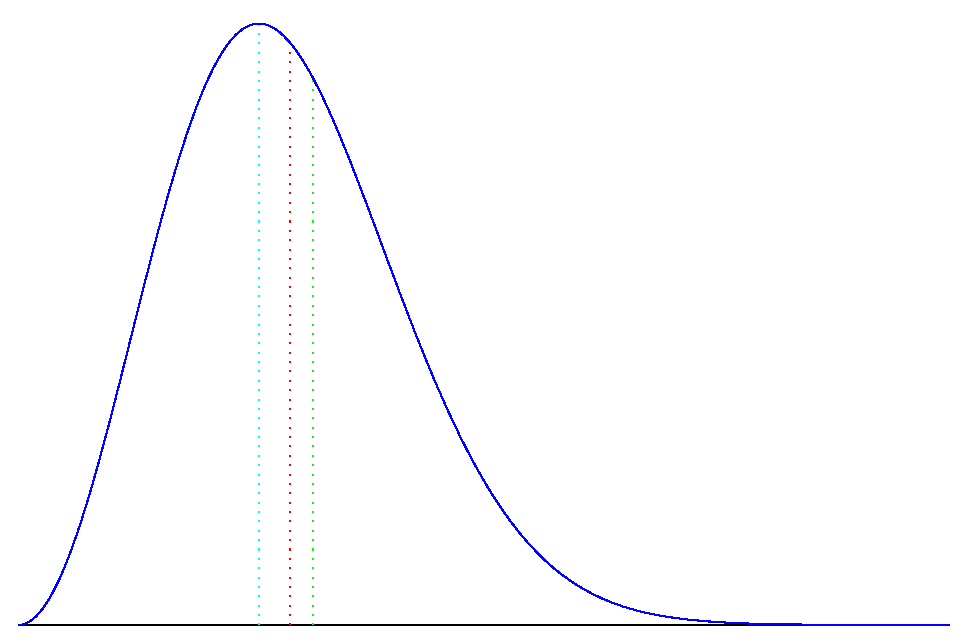
\includegraphics[scale=0.5]{immagini/fisica1/maxwell}
\caption{Distribuzione di Maxwell; velocità più probabile(blu), velocità media(rossa), velocità quadratica media(verde).}
\end{figure}
La velocità più probabile è quella in corrispondenza della quale la distribuzione ha un massimo, quindi:
\[4\pi N\frac{\ud}{\ud v}\left(\frac{m}{2\pi kT}\right)^{\frac{3}{2}}v^2e^{-\frac{mv^2}{2kT}}=0\]
\[2ve^{-\frac{mv^2}{2kT}}-\frac{v^3m}{kT}e^{-\frac{mv^2}{2kT}}=0\]
\[e^{-\frac{mv^2}{2kT}}v\left(2-v^2\frac{m}{kT}\right)=0\]
\begin{equation}
v_p=\sqrt\frac{2kT}{m}=\sqrt\frac{2RT}{M}
\end{equation}
Usando la velocità più probabile la distribuzione di Maxwell può essere scritta come:
\begin{equation}
 N(v) = \frac{4}{\sqrt{\pi}v_p^3}N v^2 e^{-v^2/v_p^2}
\end{equation}
\subsubsection{Velocità media\index{velocità!media}}
\begin{equation}
\media{v}=\frac{1}{N}\int_0^\infty vN(v)\ud v=\sqrt\frac{8kT}{\pi m}
\end{equation}

\subsubsection{Velocità quadratica media\index{velocità!quadratica media}}
\begin{equation}
\media{v^2}=\frac{1}{N}\int_0^\infty v^2N(v)\ud v=\frac{3kT}{m}
\end{equation}
\[v_\text{qm}=\sqrt{\media{v^2}}\]



\begin{figure}[htbp]
\centering
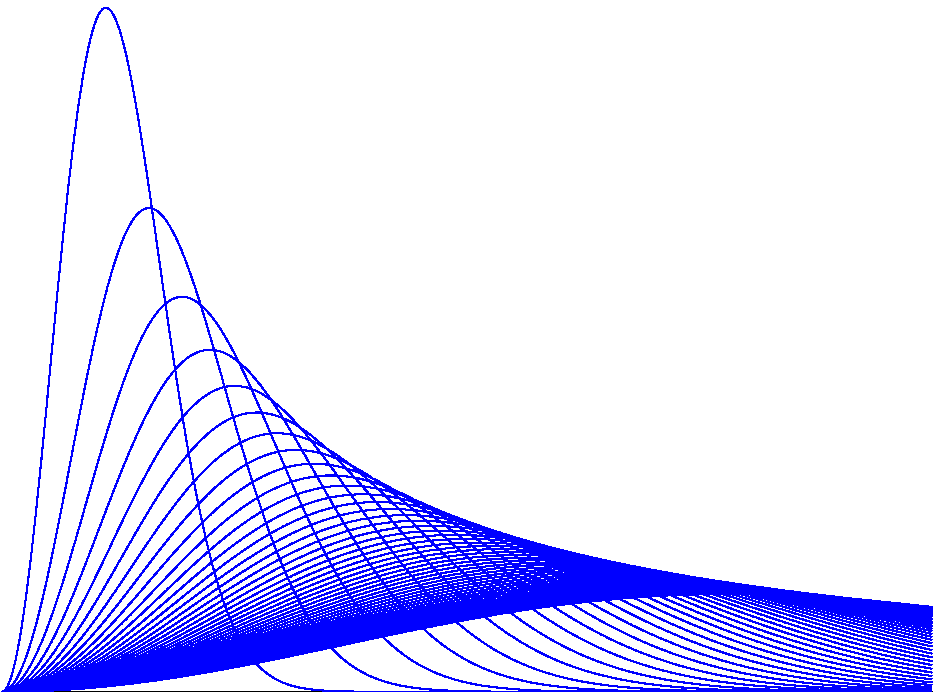
\includegraphics[scale=0.7]{immagini/fisica1/maxwell_famiglia2}
\caption{Famiglia di distribuzioni di Maxwell disegnate a intervalli costanti di temperatura.}
\end{figure}

\begin{figure}[htbp]
\centering
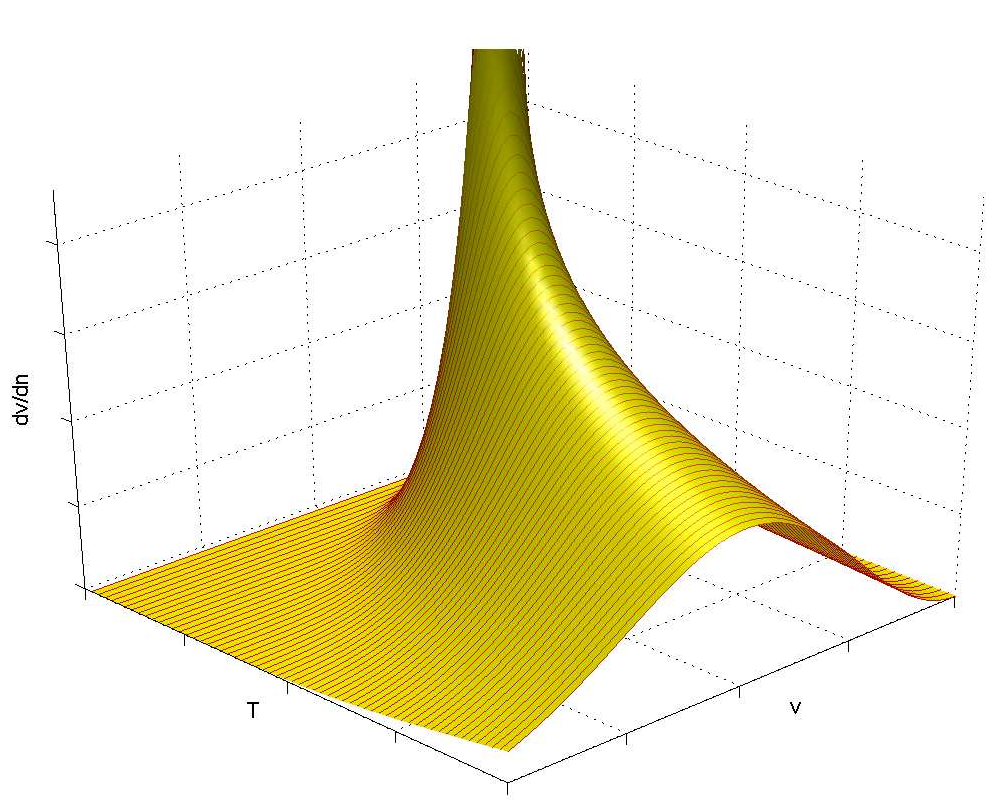
\includegraphics[scale=0.8]{immagini/fisica1/maxwell3d}
\caption{Andamento delle distribuzioni di Maxwell in funzione della temperatura.}
\end{figure}

\subsection{Distribuzione dell'energia\index{distribuzione!dell'energia}}
\begin{figure}[htbp]
\centering
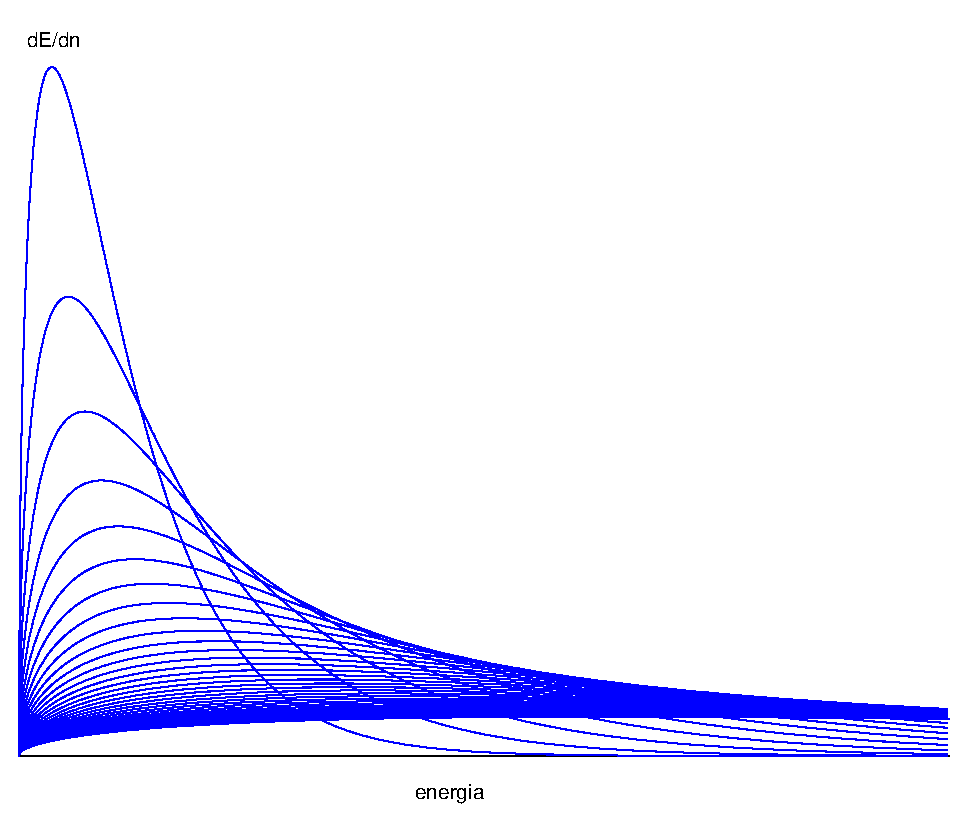
\includegraphics[scale=0.7]{immagini/fisica1/energia_max}
\caption{Famiglia di distribuzioni di energia disegnate a intervalli costati di temperatura.}
\end{figure}

Una molecola monoatomica di una gas ha solo energia cinetica $E=\frac{1}{2}mv^2$
\[v=\sqrt{\frac{2}{m}E}\]
Il numero di molecole che ha una certa velocità è uguale al numero di molecole che ha una certa energia:
\[N(E)\ud E=N(v)\ud v\]
\[N(E)=N(v)\frac{\ud v}{\ud E}=N(v)\sqrt\frac{2}{m}\frac{1}{2}E^{-\frac{1}{2}}\]
Distribuzione Maxwell--Boltzmann dell'energia:
\begin{equation}
N(E)=\frac{2N}{\sqrt{\pi}}\frac{1}{(kT)^{\frac{3}{2}}}\sqrt{E}e^{-\frac{E}{kT}}
\end{equation}
è indipendente dalla massa delle molecole, infatti un aumento di $m$ consegue una diminuzione di $v^2$ in modo che l'energia cinetica rimanga invariata.
\begin{figure}[htbp]
\centering
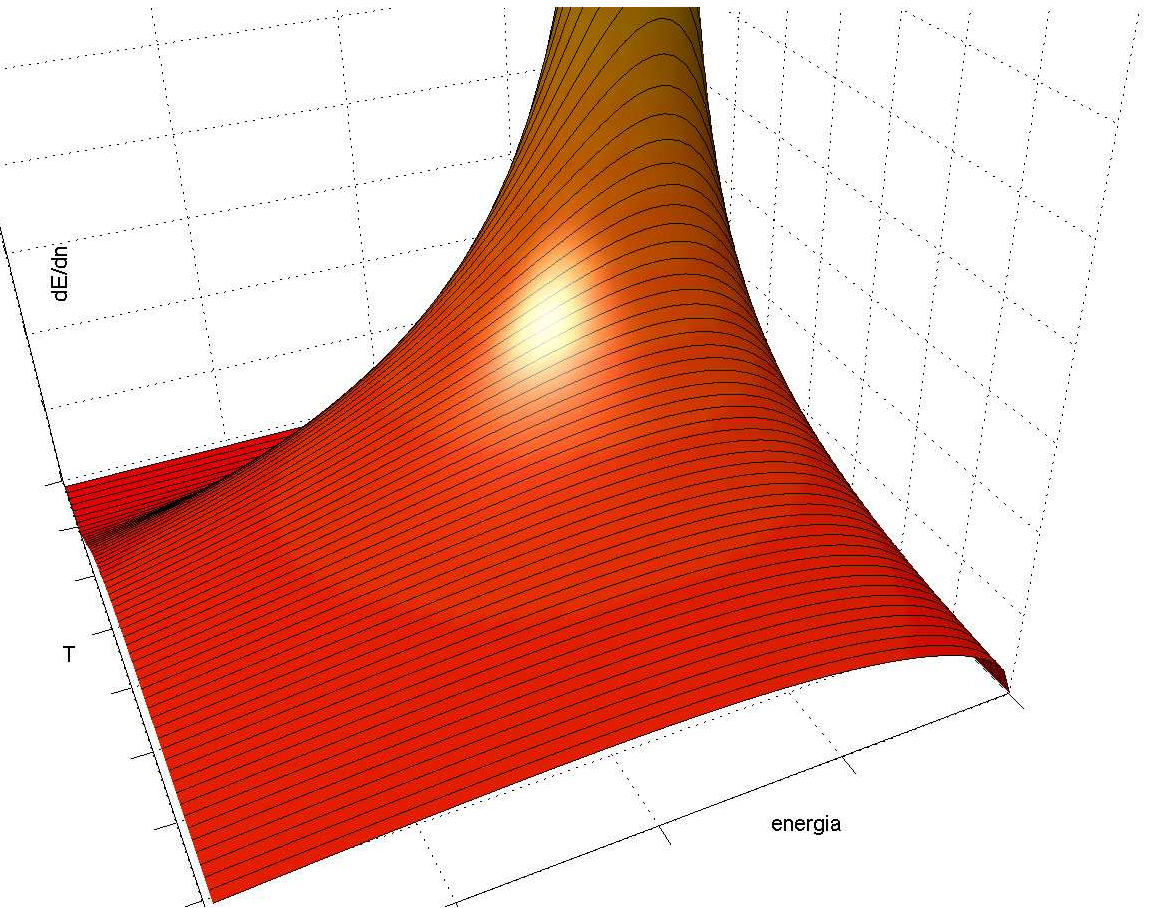
\includegraphics[scale=0.7]{immagini/fisica1/energia_max3d}
\caption{Andamento delle distribuzioni dell'energia in funzione della temperatura.}
\end{figure}

\subsubsection{Energia media\index{energia!media}}
Per un gas monoatomico
\begin{equation}
\media E=\frac{1}{N}\int_0^\infty E N(E)\ud E=\frac{3}{2}kT
\end{equation}
Per gli altri gas: $f$ numero di gradi di libertà
\begin{equation}
\media E=\frac{f}{2}kT
\end{equation}

\subsection{Riassunto teoria cinetica dei gas perfetti}
\begin{tabular}{lc}
massa molare&$M=N_A m$\\
pressione&$p=\frac{1}{3}\rho\media{v^2}$\\
velocità quadratica media&$v_\text{qm}=\sqrt\frac{3p}{\rho}=\sqrt\frac{3RT}{M}$\\
velocità più probabile&$v_p=\sqrt\frac{2RT}{M}$\\
velocità media&$\media{v}=\sqrt\frac{8RT}{\pi M}$\\
libero cammino medio&$\lambda=\frac{kT}{\sqrt{2}\pi d^2p}$\\
energia cinetica traslazionale \\per molecola monoatomica&$K=\frac{3}{2}kT$\\
\end{tabular}



\section{Trasferimenti di calore\index{trasferimento di calore}}
\subsection{Irraggiamento\index{irraggiamento}}
Ogni corpo emette radiazione elettromagnetica che dipende dalla temperatura. Leggi del corpo nero:
\begin{equation}P=\sigma T^4\qquad \lambda_\text{max}\sim\frac{1}{T}\end{equation}

\subsection{Conduzione\index{conduzione}}
Trasporto di calore senza trasporto di materia, è caratteristico dei solidi.
\begin{equation}
P=\frac{Q}{\Delta t}=K\frac{A}{\Delta x}\Delta T
\end{equation}
con $K$ coefficiente di conducibilità termica, $A$ l'area effettiva di contatto, $\Delta x$ lo spessore separatore.

\subsection{Convezione\index{convezione}}
Trasporto di calore con trasporto di materia, cioè con correnti convettive in movimento.


\section{Capacità termiche\index{capacità!termica}}
\begin{Def}[capacità termica]
Definiamo la capacita termica $C$ di un corpo la quantità di calore necessaria per far aumentare la sua temperatura di $\Delta T$:
\begin{equation}
C=\frac{Q}{\Delta T}
\end{equation}
\end{Def}
\begin{Def}[capacità termica specifica]
Definiamo la capacità termica specifica\index{capacità!termica!specifica} di una sostanza la quantità di calore necessaria per far aumentare  temperatura di $\Delta T$ un'unità di massa:
\begin{equation}
c=\frac{Q}{m\Delta T}=\frac{C}{m}
\end{equation}
\end{Def}
Esse non sono costanti, dipendono spesso dalla temperatura e dal tipo di trasformazione. Quindi al posto di $Q=mc\Delta T$ bisognerebbe scrivere:
\begin{equation}
Q=m\int_{T_0}^{T_f}c(T)\,\ud T
\end{equation}
conoscendo però come varia $c$ in funzione di $T$. Essendo $c$ variabile dal tipo di trasformazione per i gas si parla di $c_V$ calore specifico a volume costante e $c_p$ calore specifico a pressione costante.
\begin{Def}[calore specifico molare]
Il calore specifico molare è definito come\index{capacità!termica!molare}\index{calore specifico}:
\begin{equation}
c^{\text{mol}}=\frac{Q}{\Delta T n}=\frac{Q}{\Delta T}\frac{M}{m}=cM
\end{equation}
con $M=\frac{m}{n}$ massa molare\index{massa!molare}, $n$ numero di moli. Spesso $c^{\text{mol}}$ è indicato semplicemente con $c$.
\end{Def}

\index{Doulong}\index{Petit}Doulong e Petit osservarono che il calore specifico molare o capacità termica molare è uguale per tutti i solidi è circa $\si{25}{\joule\per\mole\per\kelvin}$. In realtà questo è il valore limite a cui tendono i solidi per temperature alte. Per temperature tendenti allo zero assoluto la capacità termica molare dei solidi tende a zero.


\section{Energia interna\index{energia!interna}}
L'energia interna di un gas perfetto è data solo dall'energia cinetica in quanto si è supposto che non ci sia energia potenziale. Per una molecola monoatomica $K=\frac{3}{2}kT$, per $n$ moli $E=K_n=nN_A\frac{3}{2}kT=\frac{3}{2}nRT$. Le molecole non puntiformi hanno anche energia cinetica rotazionale. Una molecola che possa ruotare su tutti i tre assi ha energia interna:
\[E=K=\frac{1}{2}mv_x^2+\frac{1}{2}mv_y^2+\frac{1}{2}mv_z^2+\frac{1}{2}I_x\omega_x^2+\frac{1}{2}I_y\omega_y^2+\frac{1}{2}I_z\omega_z^2\]
La molecola ha quindi 6 gradi di libertà, 3 traslatori e 3 rotazionali. Una molecola monoatomica ha solo 3 gradi traslatori e nessuno rotazionale in quanto essendo puntiforme $I=0$, una molecola biatomica ha 5 gradi di libertà.
\subsection{Principio di equipartizione dell'energia\index{principio!di equipartizione!dell'energia}}
Il principio di equipartizione dell'energia di Maxwell\index{Maxwell} dice che mediamente l'energia si ripartisce in modo equo tra i gradi di libertà. Ogni grado di libertà riceve $\frac{1}{2}kT$ di energia.
\begin{Pri}[equipartizione dell'energia]
\begin{equation}
E=\frac{f}{2}nRT
\label{equipartizione_00}
\end{equation}
con $f$ il numero di gradi di libertà delle particelle.
\end{Pri}
Si deduce che l'energia interna di un gas dipende esclusivamente dalla temperatura.
\subsection{Calore specifico molare dei solidi\index{capacità!termica!dei solidi}\index{calore specifico!dei solidi}}
Gli atomi dei solidi sono disposti secondo strutture reticolari e possono vibrare intorno alle loro posizioni di equilibrio in tre direzioni. Ogni atomo dispone anche di energia potenziale, quindi altri tre gradi di libertà. Avendo in totale 6 gradi di libertà dall'equazione \eqref{equipartizione_00} si ha:
\[E=3nRT\]
Se forniamo $Q$ calore al solido esso si trasformerà tutto in energia interna non compiendo il solido alcun lavoro:
\[Q=\Delta E=3nR\Delta T=nc\Delta T\]
\[c=\frac{3nR\Delta T}{n\Delta T}=3R\simeq \si{25}{\joule\per\mole\per\kelvin} \]
come previsto da Doulong\index{Doulong} e Petit\index{Petit}.
\subsection{Calore specifico dei gas\index{calore specifico!dei gas}\index{capacità!termica!dei gas}}
Come dimostrato più avanti in una trasformazione isocora tutto il calore si trasforma in variazione di energia interna in quanto non si compie lavoro.
\[c_V=\frac{Q}{n\Delta T}=\frac{\Delta E}{n\Delta T}=\frac{\frac{f}{2}nR\Delta T}{n\Delta T}=\frac{f}{2}R\]
\[c_p=c_V+R\quad\text{vedi relazione di Mayer \ref{mayer} pag.\pageref{mayer}}\]

\section{Primo principio della termodinamica\index{primo principio della termodinamica}\index{principio!primo della termodinamica}}
Consideriamo positivo qualsiasi cosa aumenti l'energia interna quindi consideriamo positivo il lavoro compiuto dall'ambiente sul sistema e positivo il calore ceduto dall'ambiente al sistema.
\[\Delta E=Q+L=E_f-E_i\]
con $E_f$, $E_i$ l'energia interna del sistema finale ed iniziale; $\Delta E$ dipende solo dalla situazione finale ed iniziale del sistema (per un gas solo dalla temperatura), quindi è una funzione di stato\index{funzione!di stato}, cioè una funzione che non dipende dalla particolare trasformazione, dal cammino percorso, ma solo dalle situazioni iniziali e finali. Mentre $L$ e $Q$ non sono funzioni di stato, la loro somma lo è. Questo è il primo principio della termodinamica:
\begin{Pri}[primo principio della termodinamica]
\begin{subequations}
\begin{equation}
Q+L=\Delta E
\end{equation}
considerando variazioni infinitesime diventa:
\begin{equation}
\delta Q+\delta L=\ud E
\end{equation}
\end{subequations}
$\ud E$ è un differenziale esatto essendo $E$ una funzione di stato.
\end{Pri}

\section{Trasformazioni di un gas\index{trasformazioni!di un gas}}
Le trasformazioni le possiamo dividere in due gruppi:
\begin{description}
\item[trasformazioni irreversibili]\index{trasformazioni!irreversibili} sono veloci, non sono determinate negli stati intermedi.
\item[trasformazioni quasistatiche]\index{trasformazioni!quasistatiche} sono lente, si dà il tempo al sistema di reagire attraversando infiniti stati di equilibrio intermedi. Una trasformazione quasi statica molto lenta idealizza una trasformazione reversibile, cioè una trasformazione che può tornare allo stato di partenza\index{trasformazioni!reversibili}.
\end{description}

\subsection{Calcolo del lavoro\index{lavoro!su un gas}}
Considerando una trasformazione reversibile e un gas perfetto:
\[\delta L=-F\ud x=-pA\ud x=-p\,\ud V\]
\begin{equation}
L=-\int_{V_0}^{V_f} p\,\ud V
\label{lavoro_gas02}
\end{equation}
Il modulo del lavoro è dunque, considerando il significato geometrico dell'integrale definito, l'area sottesa dalla curva $p=p(V)$. Il meno nella formula \eqref{lavoro_gas02} deriva dal fatto che considerando positivo il lavoro dell'ambiente la forza (dell'ambiente sul sistema) comprime il sistema, per esempio un contenitore con un pistone mobile, quindi lo spostamento è $-\ud x$, perché $x$ diminuisce.
\[\begin{array}{l}
L<0 \Leftrightarrow \text{espansione}\\
L>0 \Leftrightarrow \text{compressione}\\
\end{array}\]

In generale la forza di pressione non è una forza conservativa. Calcoliamo il lavoro svolto tra due condizioni termodinamiche, corrispondenti a due punti nel piano $pV$ attraverso due percorsi diversi (vedi figura~\ref{fig:forza_pressione}). Passiamo da $A$ a $D$ prima attraverso una isocora che faccia aumentare la pressione, da $A$ a $B$ e poi attraverso una isobara che faccia aumentare il volume, da $B$ a $D$. Il lavoro totale sarà la somma del lavoro lungo l'isocora $AB$ e dell'isobara $BD$. Il primo è nullo essendo la variazione di volume nulla. Il secondo è $\int_{V_i}^{V_f} p\ud V=p_f \Delta V$. Questo è anche il lavoro totale. Proviamo invece a calcolare il lavoro facendo prima una isobara e poi un'isocora. Il lavoro totale sarà: $p_i\Delta V$ diverso dal risultato precedente. Quindi la forza non è conservativa\footnote{se la forza fosse conservativa il lavoro in un ciclo sarebbe nullo e non sarebbe possibile realizzare le macchine termiche}.
\begin{figure}[htbp]
 \centering
% \input{immagini/fisica1/forza_pressione}
 \label{fig:forza_pressione}
\end{figure}

\subsubsection{Isobara $p=\const$}
\begin{equation}
L=-\int_{V_0}^{V_f} p\,\ud V=-p\Delta V
\end{equation}
\subsubsection{Isocora $V=\const$}
\begin{equation}
L=-\int_{V_0}^{V_f} p\,\ud V=0
\end{equation}
\subsubsection{Isoterma $T=\const$}
\begin{equation}
L=-\int_{V_0}^{V_f} p\,\ud V=-\int_{V_0}^{V_f} \frac{nRT}{V}\ud V=-nRT\int_{V_0}^{V_f} \frac{\ud V}{V}=-nRT\log\frac{V_f}{V_0}
\end{equation}
\subsubsection{Adiabatica $Q=0$}
\begin{equation}
L=\Delta E
\end{equation}
\subsection{Relazione di Mayer\index{Mayer}\index{relazione!di Mayer}}
\label{mayer}
Mostriamo la relazione tra $c_V$ e $c_p$. Consideriamo una trasformazione isocora e una isobara che partono dalla stessa situazione iniziale, e arrivano in configurazioni diverse, ma con la stessa temperatura:
\begin{figure}[htbp]
\centering
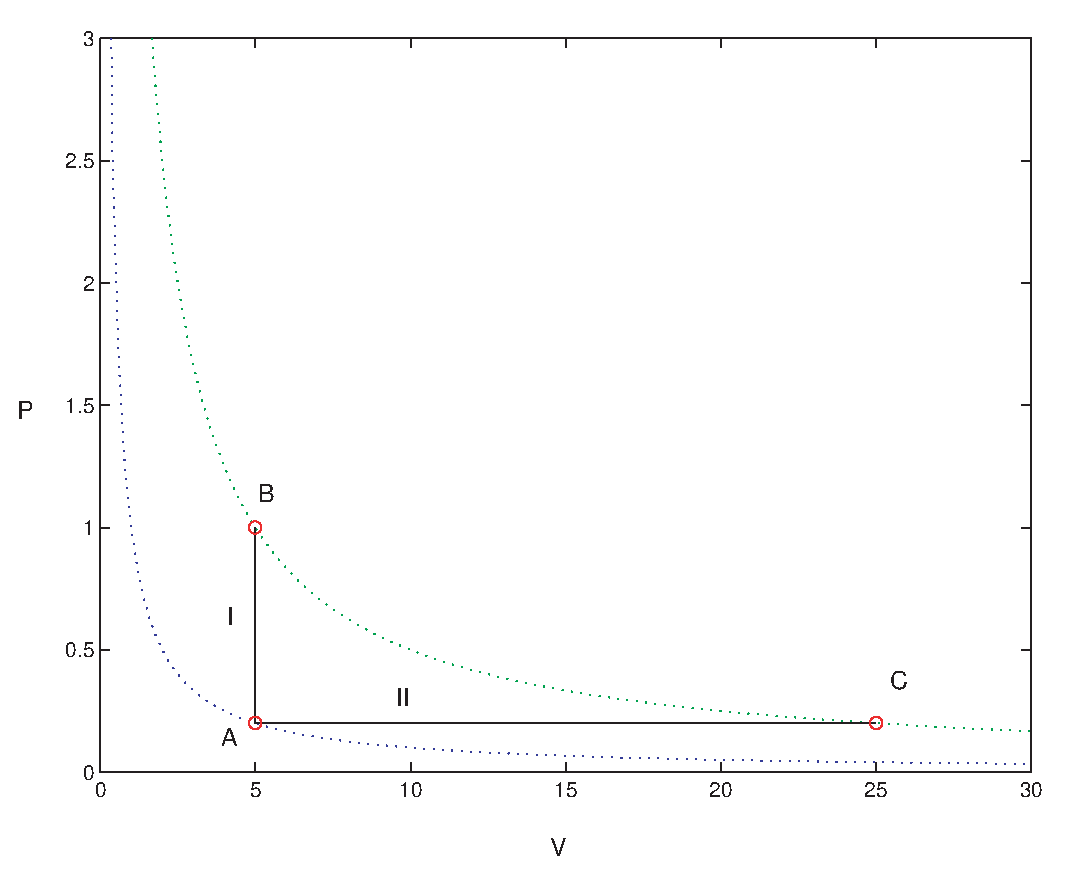
\includegraphics[scale=0.5]{immagini/fisica1/pV2_win}
\end{figure}
\begin{align*}
A\rightarrow B&\quad&V=\const&\quad&\text{I}\\
A\rightarrow C&\quad&p=\const&\quad&\text{II}
\end{align*}
\[\Delta E_I=Q_I+L_I=Q_I=nc_V\Delta T\]
\[\Delta E_{II}=Q_{II}+L_{II}=nc_p\Delta T-p\Delta V\]
$E_B=E_h$ perché $E$ dipende solo da $T$, quindi:
\[\Delta E_I=\Delta E_{II}\]
\[nc_V\Delta T=nc_p\Delta T-p\Delta V\]
\[nc_V\Delta T=nc_p\Delta T-nR\Delta T\]
\begin{Teo}[Relazione di Mayer]
 \begin{equation}
  c_p-c_V=R
 \end{equation}
\end{Teo}

\subsection{Adiabatiche}
\[Q=0\qquad \ud E=\delta Q+\delta L=\delta L=-p\ud V\]
per una isocora che lavora alle stesse temperature $\ud E=\delta Q=nc_V\ud T$
\[nc_V\ud T=-p\ud V=-\frac{nRT}{V}\ud V\]
\[c_V\ud T=-\frac{RT}{V}\ud V\]
\[\int_{T_i}^{T_f}\frac{c_V}{T}\,\ud T=-\int_{V_i}^{V_f}\frac{R}{V}\ud V\]
\[c_V\log\frac{T_f}{T_i}=-R\log\frac{V_f}{V_i}\]
\[R=c_p-c_V\qquad \gamma=\frac{c_p}{c_V}>1\]
\[\log\frac{T_f}{T_i}=\frac{c_V-c_p}{c_V}\log\frac{V_f}{V_i}=(1-\gamma)\log\frac{V_f}{V_i}\]
\[\log\frac{T_f}{T_i}=\log\left(\frac{V_f}{V_i}\right)^{\left(1-\gamma\right)}\]
\[\frac{T_f}{T_i}=\left(\frac{V_f}{V_i}\right)^{\left(1-\gamma\right)}\qquad T_fV_f^{\gamma-1}=T_iV_i^{\gamma-1}\qquad\]
\[TV^{\gamma-1}=\const\]
usando $PV=nRT$ e quindi $T=\const PV$:
\[PVV^{\gamma-1}=\const\]
\begin{equation}
PV^\gamma=\const\quad\text{Relazione di Poisson}
\end{equation}

\begin{Es}[Gradiente termico atmosferico]
L'aria è un cattivo conduttore termico, quindi quando delle masse d'aria a temperatura diversa si spostano si può considerare la trasformazione come adiabatica. La pressione atmosferica descresce con la quota, vedi \eqref{legge_atmosfera}. Per la legge di Archimede l'aria calda più leggera sale si espande a causa delle minore temperatura. Essendo la trasformazione adiabatica non c'è scambio di calore. Essendoci un'espansione la massa d'aria compie lavoro a scapito dell'energia interna, e quindi la temperatura diminuisce.

Per la legge di Stevino:
\[
 \ud P = -\rho g \ud h = -\frac{M}{V} g \ud h = -\frac{MP}{nRT} g \ud h
\]
dove abbiamo usato la legge dei gas perfetti ($PV=nRT$). Per le trasformazioni adiabatiche $TV^{\gamma-1}=\const$, allora $T^\gamma P^{1-\gamma} = \const$ e quindi possiamo collegare le variazioni di pressione alle variazioni di temperatura:
\[ T^{\gamma} P^{1-\gamma} = \const\]
\[ T = \const P^{\frac{\gamma - 1}{\gamma}}\]
\[ \log T = \frac{\gamma - 1}{\gamma} \log P + \const\]
\[\frac{1}{T}\frac{\ud T}{\ud P} = \frac{\gamma - 1}{\gamma} \frac{1}{P} \]
\[\frac{\ud T}{T} = \frac{\gamma - 1}{\gamma} \frac{\ud P}{P} \]
sostituendo:
\[
 \frac{\ud T}{\ud h} = -\frac{\gamma -1}{\gamma} \frac{Mg}{nR}
\]
Assumendo $\gamma = \frac{c_v+R}{c_v} = \frac{7}{5}$ (gas biatomico, $c_v = \frac{5}{2}R$) e la massa molare $\frac{M}{n} = \SI{28.88}{\gram\per\mol}$ si ottiene un gradiente costante:
\[
 \frac{\ud T}{\ud h} \simeq -\SI{9.74}{\kelvin\per\kilo\meter}
\]
questo gradiente è abbastanza più grande del grandiente osservato in quando si è trascurato la presenza di vapore acqueo che condensandosi al diminuire della temperatura sottrae calore sotto forma di calore latente.
\end{Es}


\subsection{Trasformazioni politropiche\index{trasformazioni!politropiche}}
Nelle trasformazioni politropiche $c$ è ritenuto costante.
\[\ud E=\delta Q+\delta L=nc\ud T-p\ud V\]
Il ragionamento è simile a quanto fatto con le adiabatiche; consideriamo una trasformazione isocora che lavora tra le stesse temperature $\ud E=nc_V\ud T$
\[nc\ud T-p\ud V=nc_V\ud T\]
\[nc\ud T-\frac{nRT}{V}\ud V=nc_V\ud T\]
\[(c_V-c)\ud T=-\frac{RT}{V}\ud V\quad \int_{T_0}^{T_f}\frac{c_V-c}{T}\ud T=-\int_{V_0}^{V_f}\frac{R}{V}\ud V\]
\[(c_V-c)\int_{T_0}^{T_f}\frac{\ud T}{T}=-R\int_{V_0}^{V_f}\frac{\ud V}{V}\]
\[\int_{T_0}^{T_f}\frac{\ud T}{T}=-\frac{c_p-c_V}{c_V-c}\int_{V_0}^{V_f}\frac{\ud V}{V}\]
\[\log\frac{T_f}{T_0}=-\frac{c_p-c_V}{c_V-c}\log\frac{V_f}{V_0}=\frac{c_p-c_V}{c_V-c}\log\frac{V_0}{V_f}\]
\[(k-1)=\frac{c_p-c_V}{c_V-c}\]
\[\log\frac{T_f}{T_0}=\log\left[\left(\frac{V_0}{V_f}\right)^{k-1}\right]\qquad\frac{T_f}{T_0}=\left(\frac{V_0}{V_f}\right)^{k-1}\]
\[T_fV_f^{k-1}=T_0V_0^{k-1}\qquad TV^{k-1}=\const\]
\[PVV^{k-1}=(nR)\const\qquad PV^k=\const\]
\[k=\frac{c_p-c}{c_V-c}\qquad c=\frac{kc_V-c_p}{k-1}\]
\subsubsection{Tutte le trasformazioni come politropiche}
\begin{center}
\begin{tabular}{l|ccc}
Isoterma&$pV=\const$&$k=1$&$c=\infty$\\
Isocora&$V=\const$&$k=\infty$&$c=c_V$\\
Isobara&$p=\const$&$k=0$&$c=c_p$\\
Adiabatica&$pV^\gamma=\const$&$k=\gamma>1$&$c=0$\\
\end{tabular}
\end{center}

\begin{figure}[htbp]
\centering
\subfigure[$c$ in funzione di $k$]{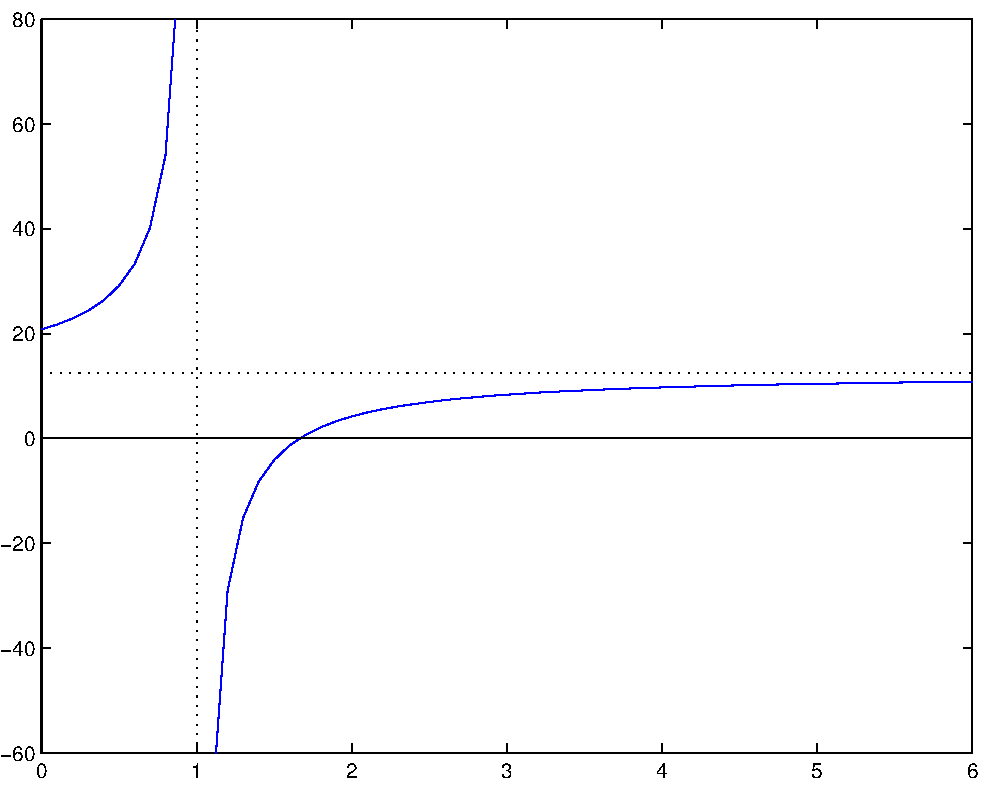
\includegraphics[scale=0.4]{immagini/fisica1/ck2}}
\subfigure[isoterma e adiabatiche in un grafico $p(V)$, quelle intermedie hanno \mbox{$c<0$}]{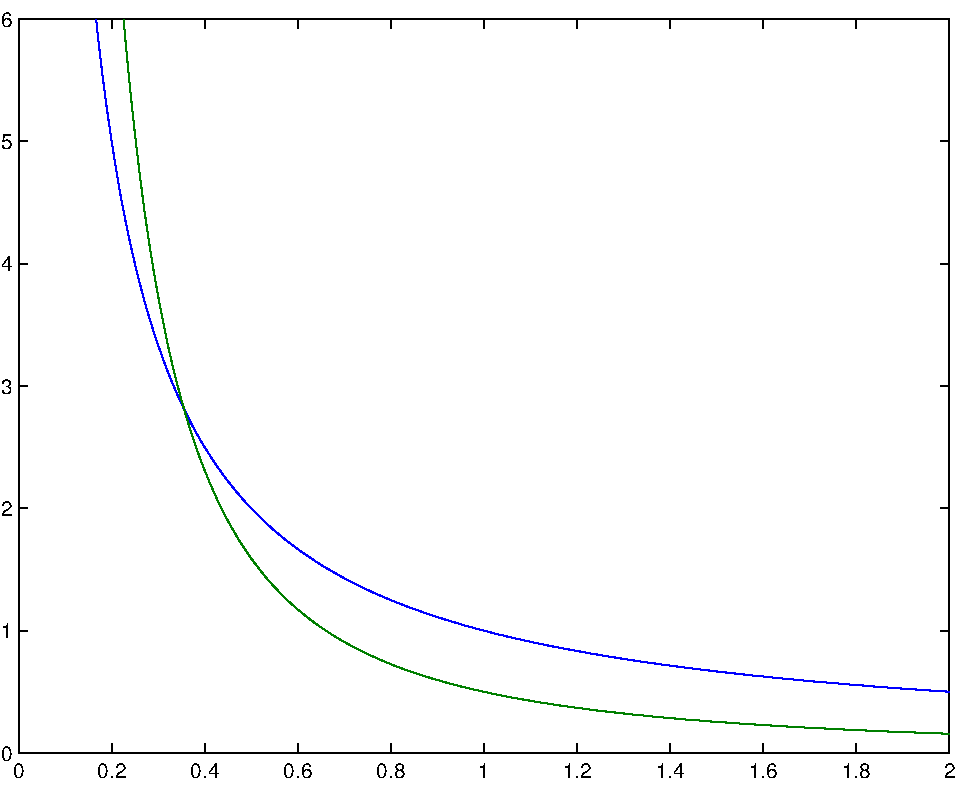
\includegraphics[scale=0.4]{immagini/fisica1/pvv2}}
\end{figure}

\begin{center}
\begin{tabular}{lccc}
&$L$&$Q$&$\Delta E$\\
\hline
Isoterma&$-nRT\log\frac{V_f}{V_0}$&$nRT\log\frac{V_f}{V_0}$&$nc_V\Delta T=0$\\
Isocora&$0$&$nc_V\Delta T$&$nc_V\Delta T$\\
Isobara&$-p\Delta V$&$nc_p\Delta T$&$nc_V\Delta T$\\
Adiabatica&$nc_V\Delta T$&$0$&$nc_V\Delta T$\\
\end{tabular}
\end{center}
\section{Entalpia}
\begin{Def}[Entalpia]
 \begin{equation}
  H = U + pV
 \end{equation}
\end{Def}
poiché $U$ è una funzione di stato e dipende solo dalla temperatura e il prodotto $pV=nRT$ dipende solo dalla temperatura, allora $H$ è una funzione di stato e dipende solo dalla temperatura.

L'entalpia è legata al calore specifico a pressione costante:
\begin{equation}
 \ud H = \ud U + \ud(nRT) = nc_v\ud T + nR\ud T = nc_p\ud T
\end{equation}
quindi in generale:
\begin{equation}
 \Delta H = n\int_{T_1}^{T_2} c_p\,\ud T
\end{equation}
o semplicemente
\begin{equation}
 \Delta H = nc_p\Delta T
\end{equation}
se $c_p$ è costante al variare della temperatura. Per una isobara vale dunque:
\begin{equation*}
 Q = n\int_{T_1}^{T_2} c_p\ud T = \Delta H
\end{equation*}
mentre per una isocora valeva:
\begin{equation*}
 Q = n\int_{T_1}^{T_2}c_v\ud T = \Delta U
\end{equation*}
quindi possiamo ridefinire i calori specifici molari come:
\begin{equation}
 c_v = \frac{1}{n}\frac{\ud U}{\ud T} \qquad c_p = \frac{1}{n}\frac{\ud H}{\ud T}
\end{equation}


\section{Trasformazioni cicliche\index{trasformazioni!cicliche}}
Una trasformazione ciclica è una trasformazione in cui gli stati iniziali e finali coincidono, quindi:
\begin{equation}
\Delta E=Q+L=0
\end{equation}
La macchine termiche trasformano il calore in lavoro e il loro ciclo è chiamo \index{ciclo!termico}ciclo termico. I frigoriferi trasformano il lavoro in trasferimento di calore, dalla sorgente più fredda a quella più calda e il loro ciclo è chiamato \index{ciclo!frigorifero}ciclo frigorifero.
\subsection{Ciclo di Carnot per un gas perfetto\index{Carnot}\index{ciclo!di Carnot}\index{macchina!di Carnot}}
\begin{figure}[htbp]
\centering
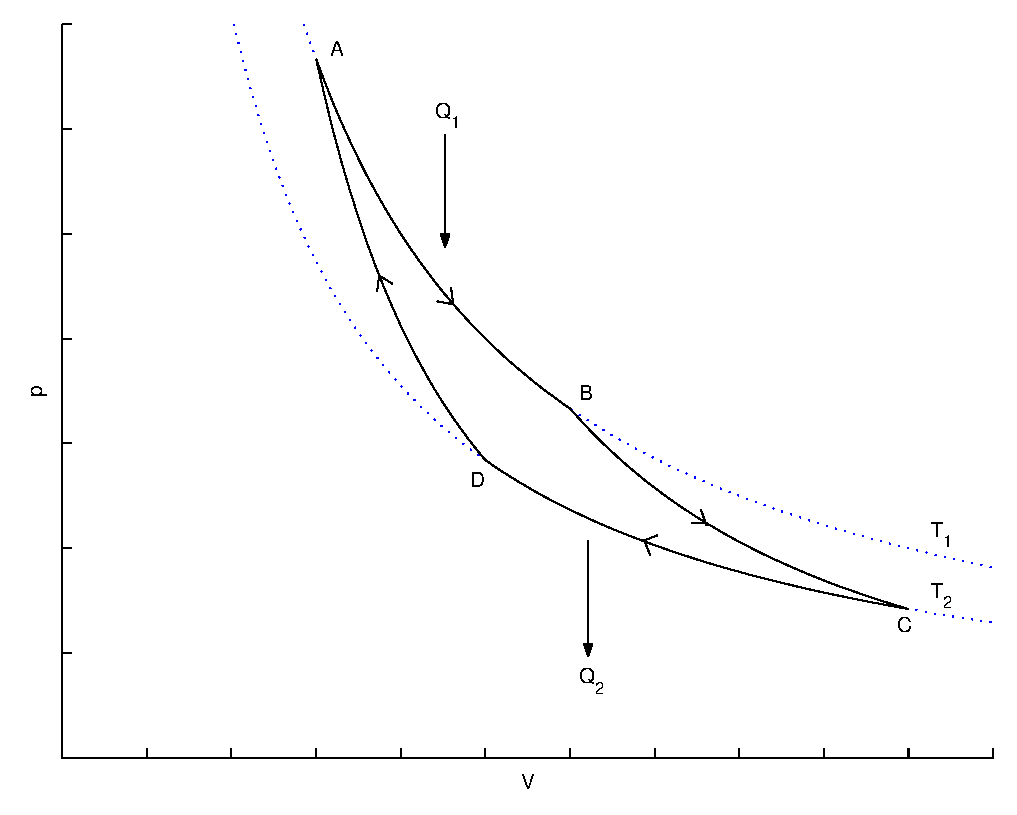
\includegraphics[scale=0.5]{immagini/fisica1/Carnot}
\caption{Ciclo di Carnot.}
\end{figure}
\parbox[]{\textwidth}{
\begin{enumerate}
\item Si porta il sistema alla temperatura $T_1$ immergendo in un bagno termico.
\item Il gas si espande da $V_A$ a $V_B$ seguendo una trasformazione isotermica.
\item Il gas si espande da $V_B$ a $V_C$ seguendo una trasformazione adiabatica.
\item Si porta il sistema alla temperatura $T_2$ immergendolo in un bagno termico.
\item Si comprime il gas da $V_C$ a $V_D$ seguendo una isoterma.
\item Si comprime il gas da $V_D$ a $V_A$ seguendo una adiabatica.
\end{enumerate}}
Nota: $Q_1>0$, $Q_2<0$, $L<0$

\[Q=Q_1-|Q_2|=-L\]
\[Q_2=nRT\log\frac{V_D}{V_C}\]
\[T_1V_B^{\gamma-1}=T_2V_C^{\gamma-1}\]
\[T_1V_A^{\gamma-1}=T_2V_D^{\gamma-1}\]
\[\left(\frac{V_B}{V_A}\right)^{\gamma-1}=\left(\frac{V_C}{V_D}\right)^{\gamma-1}\qquad \frac{V_B}{V_A}=\frac{V_C}{V_D}\]
Nella macchina di Carnot gli scambi di calore avvengono con delle isoterme, quindi i calori stanno alle temperature:
\begin{equation}
 \frac{|Q_2|}{Q_1}=\frac{nRT_2\log\frac{V_C}{V_D}}{nRT_1\log\frac{V_B}{V_A}}=\frac{T_2}{T_1}
\end{equation}

Il rendimento $\eta$ sarà maggiore quanto maggiore è il lavoro svolto dalla macchina sull'ambiente con minore scambio di calore.
\[\eta=\frac{|L|}{Q_1}=\frac{Q_1-|Q_2|}{Q_1}=1-\frac{|Q_2|}{Q_1}=1-\frac{T_2}{T_1}<1\]
La condizione migliore è quella della macchina perfetta \index{macchina!perfetta}in cui tutto il calore è trasformato in lavoro, $\eta_\text{perfetta}= 1$

\subsection{Frigorifero\index{frigorifero}\index{macchina!frigorifera}}
Si esegue il ciclo di Carnot al contrario. Si fornisce quindi lavoro e si ha un trasferimento di calore, trasferendolo dalla sorgente fredda a quella più calda.
Il coefficiente di merito sarà maggiore quando è maggiore il calore trasferito e minore il lavoro necessario.
Nota: $Q_1<0$, $Q_2>0$, $L>0$
\[0=L+Q=L+Q_2-|Q_1|\]
\[L=|Q_1|-Q_2\qquad\frac{Q_1}{Q_2}=\frac{T_1}{T_2}\]
\[\eta=\frac{Q_2}{L}=\frac{Q_2}{|Q_1|-Q_2}=\frac{T_2}{T_1-T_2}>0\]
Il frigorifero perfetto trasferisce calore dalla sorgente più fredda a quella più calda senza bisogno di lavoro, quindi $\eta\rightarrow\infty$

\subsection{Ciclo Otto\index{ciclo!Otto}}
Il ciclo Otto approssima molto il ciclo di un motore a benzina a quattro tempi.
\begin{itemize}
\item[] OA=aspirazione miscela
\item[] AB=compressione adiabatica
\item[] BC=accensione
\item[] CD=espansione adiabatica
\item[] DA=raffreddamento
\item[] OA=espulsione gas combusti
\end{itemize}

\[Q_{BC}=nc_V\Delta T=nc_V(T_C-T_B)>0\]
\[Q_{DA}=nc_V\Delta T=nc_V(T_A-T_D)<0\]
\[L+Q_{BC}-|Q_{DA}|=0 \qquad L=|Q_{DA}|-Q_{BC}<0\qquad |L|=Q_{BC}-|Q_{DA}|\]
\[\eta=\frac{|L|}{Q_{BC}}=\frac{Q_{BC}-|Q_{DA}|}{Q_{BC}}=1-\frac{|Q_{DA}|}{Q_{BC}}=1-\frac{nc_V(T_D-T_A)}{nc_V(T_C-T_B)}=1-\frac{T_D-T_A}{T_C-T_C}\]

Spesso il rendimento viene espresso in funzione del rapporto di compressione $r=\frac{V_2}{V_1}$
\[TV^{\gamma-1}=\const\]

\[\left\{
\begin{array}{l}
T_CV_1^{\gamma-1}=T_DV_2^{\gamma-1}\\
T_BV_1^{\gamma-1}=T_AV_2^{\gamma-1}\\
\end{array}\right.\]
\[(T_C-T_B)V_1^{\gamma-1}=(T_D-T_A)V_2^{\gamma-1}\]
\[\frac{T_D-T_A}{T_C-T_B}=\left(\frac{V_1}{V_2}\right)^{\gamma-1}\]

\[\eta=1-\frac{T_D-T_A}{T_C-T_B}=1-\left(\frac{V_1}{V_2}\right)^{\gamma-1}\!\!\!\!\!\!\!\!\! =1-\left(\frac{1}{r}\right)^{\gamma-1}\]

Più grande è $r$ più è grande $\eta$. Se $r$ è troppo grande $\Delta V$ è grande e nella compressione si crea troppo calore che provoca la preaccensione. Tipicamente $r=5$, quindi $\eta=0.55$. In realtà con questo rapporto di compressione nella macchine reali si ha $\eta=0.3$.

\subsection{Diagrammi di flusso}
I diagrammi di flusso sono degli schemi utili per descrivere le trasformazioni cicliche. I piani orizzontali rappresentano le fonti di calore a diversa temperatura, la sezione del tubo varia a seconda dell'energia interna del sistema.

\begin{figure}[!htbp]
\centering
\subfigure[ideale]{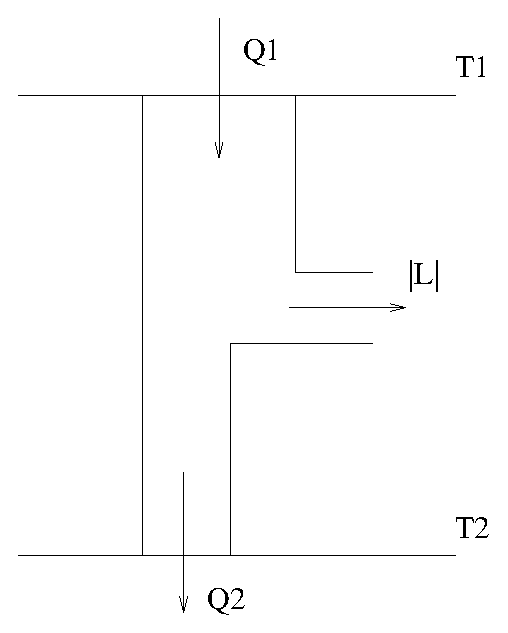
\includegraphics[scale=0.5]{immagini/fisica1/flusso_carnot}}\quad
\subfigure[perfetta]{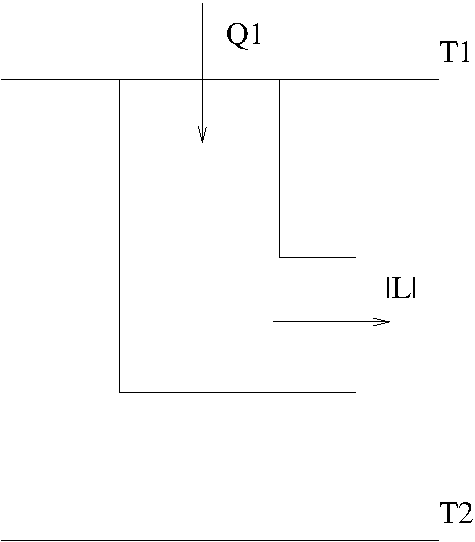
\includegraphics[scale=0.5]{immagini/fisica1/flusso_carnot_perf}}
\caption{Macchina di Carnot.}
\end{figure}
\begin{figure}[!htbp]
\centering
\subfigure[ideale]{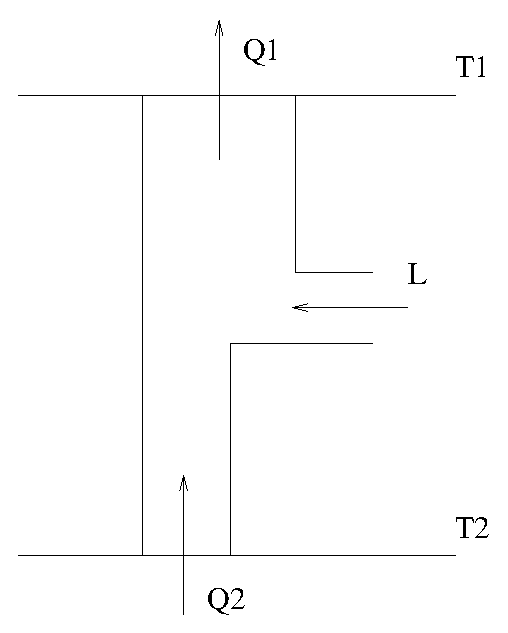
\includegraphics[scale=0.5]{immagini/fisica1/flusso_frigo}}\quad
\subfigure[perfetto]{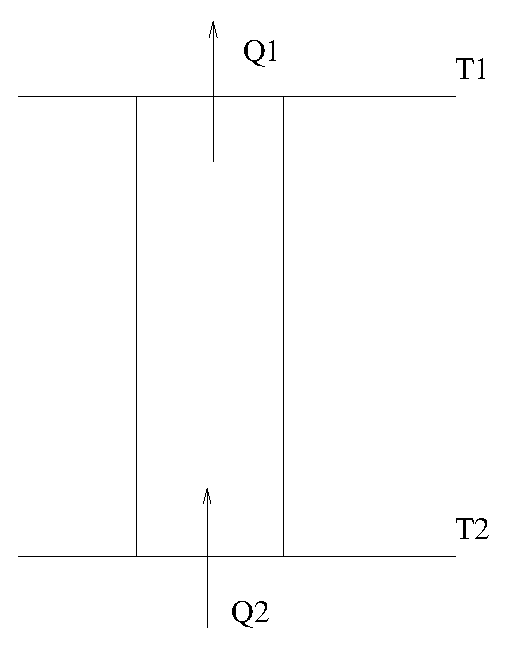
\includegraphics[scale=0.5]{immagini/fisica1/flusso_frigo_perf}}
\caption{Frigorifero.}
\end{figure}

\section{Secondo principio della termodinamica\index{secondo principio della termodinamica}\index{principio!secondo della termodinamica}}

\begin{Pri}[Enunciato di Kelvin]
\index{Kelvin}è impossibile realizzare una trasformazione il cui unico scopo è di produrre lavoro da una sola sorgente di calore.
\end{Pri}

\begin{Pri}[Enunciato di Clausius]
\index{Clausius}è impossibile realizzare una trasformazione il cui unico scopo sia quello di fare passare calore da una sorgente di bassa temperatura ad una più alta.
\end{Pri}

Una isoterma sembra violare Kelvin, in realtà trasforma tutto il calore in lavoro, ma non fa solo quello, infatti espande il gas.
\subsection{\texorpdfstring{$\text{Kelvin}\Leftrightarrow\text{Clausius}$}{Kelvin <=> Clausius}}

Chiamiamo $\bar{K}$ antikelvin un ciclo che viola Kelvin e $\bar{C}$ anticlausius un ciclo che viola Clausius. Dimostriamo che $\exists\bar{K}\Rightarrow\exists\bar{C}$ Sommiamo un antikelvin con un frigorifero e otteniamo un anticlausius (Figura \ref{CK1}). Quindi l'esistenza di un antikelvin implica l'esistenza di un anticlausius. Dopodiché $\nexists\bar{C}\Rightarrow\nexists\bar{K}$.

Sommando un anticlausius e una macchina termica e otteniamo un antikelvin (Figura \ref{CK2}), quindi
 $\exists\bar{C}\Rightarrow\exists\bar{K}$ e allora $\nexists\bar{K}\Rightarrow\nexists\bar{C}$. In definitiva abbiamo dimostrato che l'enunciato di Clausius e di Kelvin sono equivalenti.
\begin{figure}[htbp]
\centering
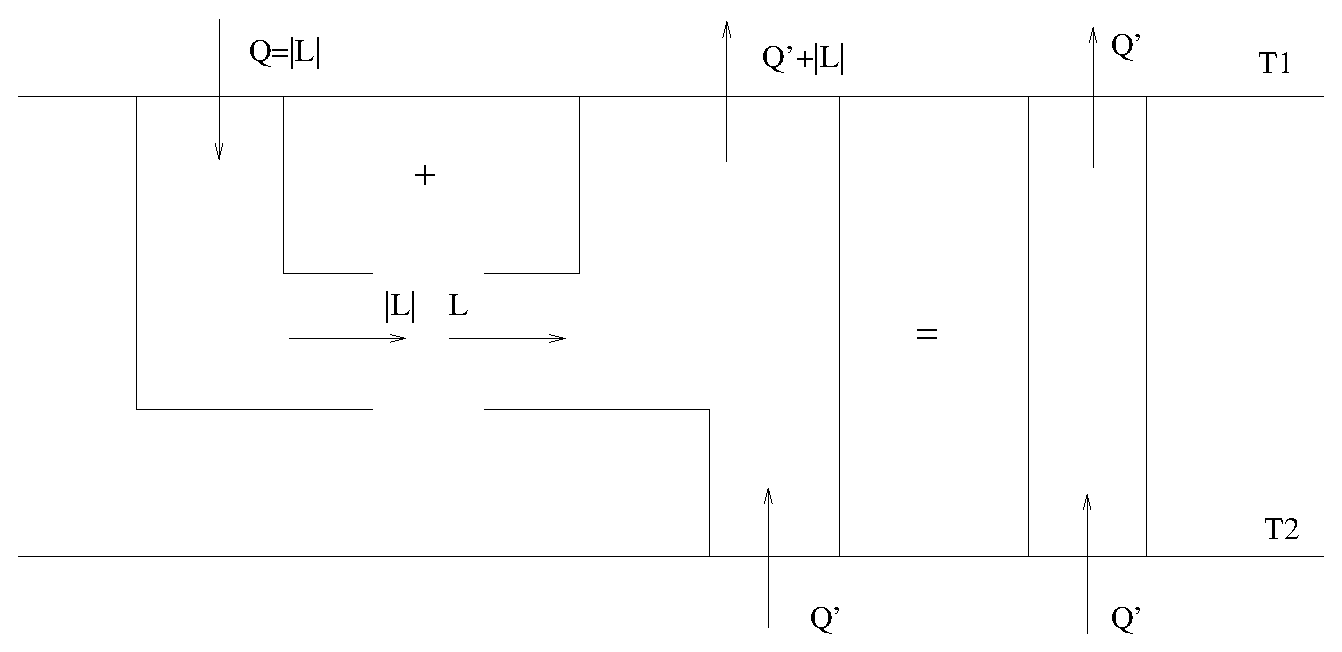
\includegraphics[scale=0.5]{immagini/fisica1/AK+Frigo}
\caption{Antikelvin più un frigorifero.}
\label{CK1}
\end{figure}

\begin{figure}[htbp]
\centering
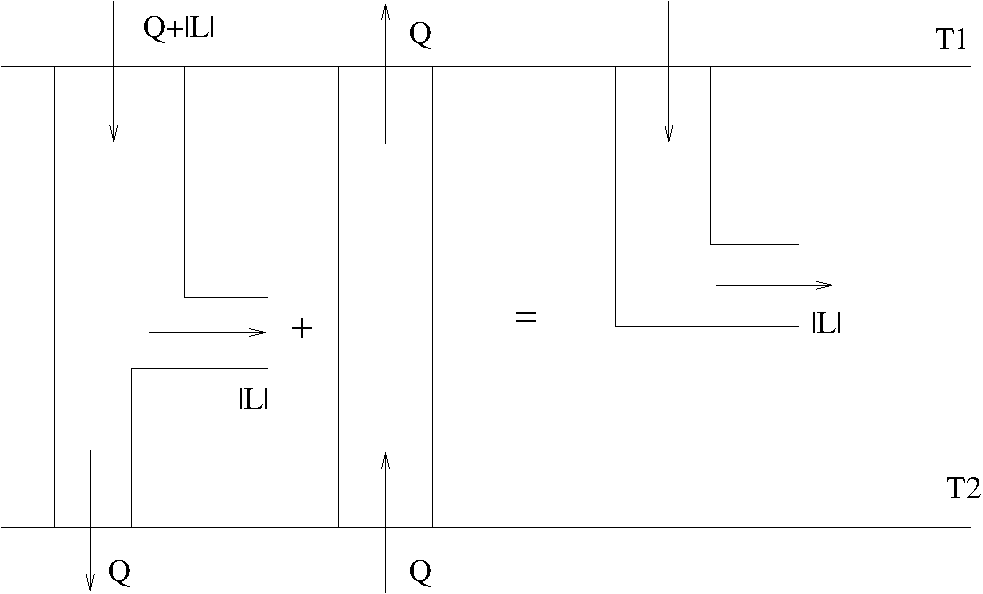
\includegraphics[scale=0.5]{immagini/fisica1/AC+Carnot}
\caption{Anticlausius più una macchina termica.}
\label{CK2}
\end{figure}

\subsection{Teorema di Carnot\index{teorema!di Carnot}}
\begin{Teo}[Carnot: il più bravo sono io]
a parità di temperature non esiste macchina con rendimento migliore di quella di Carnot: $\eta_M\leq\eta_C$.
\end{Teo}
\subsubsection{Dimostrazione caso con due sorgenti}
Per assurdo: $\exists M: \eta_M>\eta_C$. Con la macchina di Carnot posso variare a piacimento il lavoro tenendo fisso $\eta$ allungando le isoterme. Scelgo una macchina di Carnot tale che $L_C=L_M$. Le macchine lavorano alle stesse temperature per ipotesi. La macchina $M$ avendo maggior rendimento avrà bisogno di meno calore, infatti:
\[\eta_M=\frac{|L_M|}{Q_M}>\eta_C=\frac{|L_C|}{Q_C}=\frac{|L_M|}{Q_C}\]
\[\frac{|L_M|}{Q_M}>\frac{|L_M|}{Q_C} \qquad Q_M<Q_C\]

Combino la macchina $M$ con la macchina di Carnot fatta funzionare al contrario, trovo un antikelvin. Assurdo, quindi: \[\eta_M\leq\eta_C\]
\begin{figure}[htbp]
\centering
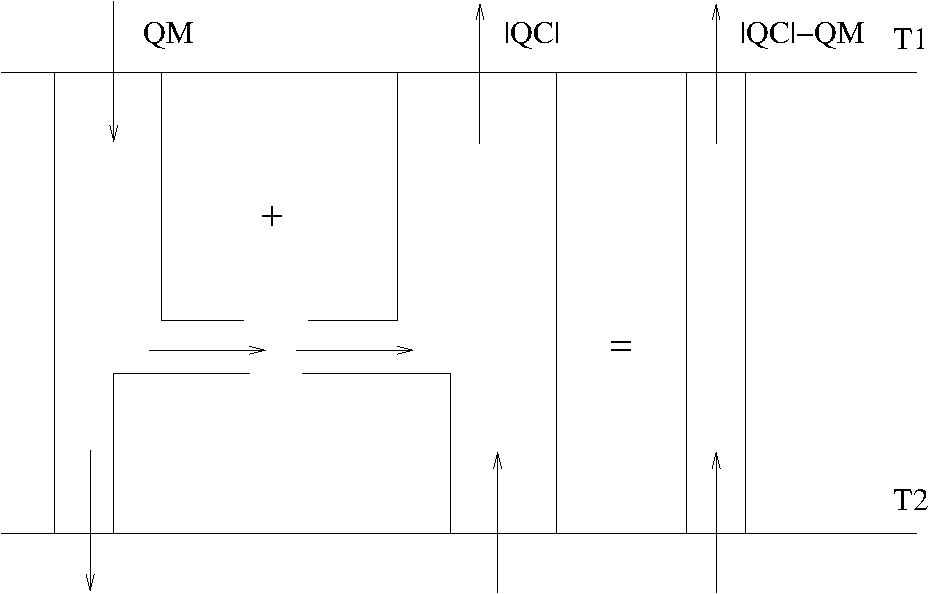
\includegraphics[scale=0.5]{immagini/fisica1/M+c-1}
\caption{Macchina $M$ più la macchina di Carnot al contrario.}
\end{figure}

\begin{Cor}
Se la macchina è reversibile $\eta_M=\eta_C$. Per assurdo $\eta_M<\eta_C$, $M^{-1}+C=\bar{C},$ assurdo $\Rightarrow \eta_M\geq\eta_C\Rightarrow \eta_M=\eta_C$
\end{Cor}

Questo significa che tutte le macchine reversibili che lavorano tra due sorgenti $T_2 > T_1$: $\eta = 1-\frac{T_1}{T_2} = 1 - \frac{|Q_1|}{Q_2}$. Allora:
\begin{equation}
 \frac{Q_1}{T_2} + \frac{Q_2}{T_2} = 0
\end{equation}
il lavoro sarà:
\begin{equation}
 L = Q_2\eta = Q_2 \left(1 - \frac{T_1}{T_2}\right)
\end{equation}




\section{Entropia\index{entropia}}
Consideriamo una trasformazione reversibile per un gas perfetto:
\[\delta Q+\delta L=\ud E\qquad \delta Q-p\ud V=nc_V\ud T\]
\[\delta Q=nc_V\ud T+p\ud V\]
\[\frac{\delta Q}{T}\;\text{è un differenziale esatto?}\]
Per verificarlo integriamo la quantità e vediamo se si può esprime come differenza di funzioni che dipendono solo dallo stato iniziale e finale del sistema e non dalla particolare trasformazione. L'integrale quindi sarà una funzione di stato.
\begin{align*}
\int_i^f\frac{\delta Q}{T}&=\int_i^f\frac{nc_V\ud T+p\,\ud V}{T}=\int_{T_i}^{T_f}\frac{nc_V\ud T}{T}+\int_{V_i}^{V_f}\frac{p\,\ud V}{T}\\
&=nc_V\int_{T_i}^{T_f}\frac{\ud T}{T}+\int_{V_i}^{V_f}\frac{\frac{nRT}{V}\ud V}{T}=nc_V\int_{T_i}^{T_f}\frac{\ud T}{T}+nR\int_{V_i}^{V_f}\frac{\ud V}{V}\\
&=(nc_V\log T_f+nR\log V_f)-(nc_V\log T_i+nR\log V_i)=S_f-S_i\\&=\Delta S
\end{align*}
\[S=nc_V\log T+nR\log V+\const=\text{entropia}\]
\[\int_i^f\frac{\delta Q}{T}=\Delta S\qquad \oint\frac{\delta Q}{T}=0\]
L'entropia è una funzione di stato. La definizione data vale solo per trasformazioni reversibili. Per una trasformazione irreversibile si può calcolare $\Delta S$ usando una trasformazione reversibile che colleghi gli stessi stati iniziali e finali (vedi esempio espansione libera).
\subsubsection{Isocora}
\[\Delta S=nc_V\log\frac{T_f}{T_i}+nR\log\frac{V_f}{V_0}=nc_V\log\frac{T_f}{T_i}\]
\subsubsection{Isobara}
\[\frac{V_i}{V_f}=\frac{T_i}{T_f}\]
\begin{align*}
\Delta S=&nc_V\log\frac{T_f}{T_i}+nR\log\frac{V_f}{V_i}=nc_V\log\frac{T_f}{T_i}+nR\log\frac{T_f}{T_i}\\
=&\log\frac{T_f}{T_i}(c_V+R)=nc_p\log\frac{T_f}{T_i}
\end{align*}
\subsubsection{Adiabatica}
\[\delta Q=0 \Rightarrow \Delta S=0\]
Le adiabatiche vengono anche chiamate trasformazioni isoentropiche
\subsubsection{Isoterma}
\[\Delta S=nc_V\log\frac{T_f}{T_i}+nR\log\frac{V_f}{V_0}=nR\log\frac{V_f}{V_0}=\frac{Q}{T}\]
\subsubsection{Espansione libera}
L'espansione libera è una adiabatica irreversibile, quindi non si può concludere che $\Delta S=0$. Lo stato iniziale e quello finale sono alla stessa temperatura, quindi si trovano sulla stessa isoterma. La trasformazione pur non essendo isoterma ha $\Delta S$ di una isoterma. Se il volume finale è il doppio di quello iniziale:
\[\Delta S=nR\log\frac{V_f}{V_i}=nR\log 2\]

\subsection{Entropia nei cicli\index{entropia!nei cicli}}
Il teorema di Clausis estende il risultato a due sorgenti dal teorema di Carnot con macchine reversibili: $\frac{Q_1}{T_1} + \frac{Q_2}{T_2} = 0$.
\begin{Teo}[Clausius]
 Consideriamo macchina generica $M$ con $n$ sorgenti di calore a temperature diverse $T_i$ dalle quali assorbe calore $Q_i$. Allora vale:
  \begin{equation}
   \sum_i \frac{Q_i}{T_i} \leq 0
  \end{equation}
l'uguaglianza vale solo se la macchina è reversibile.
\end{Teo}

Per dimostrare il teorema introduciamo $n$ macchine reversibili $C_i$, ognuna che opera tra due sorgenti, $T_i$ e $T_0$. La macchina $M$ non scambia calore con $T_0$. Le macchine reversibili $C_i$ sono tali da scambiare lo stesso calore $Q_i$ dalla sorgente a temperatura $T_i$ come la macchina $M$, ma con segno opposto. Quindi se la macchina $M$ assorbe calore $|Q_i|$ alla sorgente a temperatura $T_i$ allora $C_i$ cede $|Q_i|$ e viceversa.

Usando la relazione generica $\frac{Q_A}{T_A} + \frac{Q_B}{T_B} = 0$ si ottiene alla macchina $C_i$:
\[
 Q_{i,0} = \frac{T_0}{T_i} Q_i
\]

Consideriamo ora la $H=\text{macchina infernale}=M+\sum_{i=1}^{n}C_i$ come in figura \ref{fig:hell_machine}. Poiché i calori della macchina $M$ e $C_i$ si compensano per ogni sorgente a temperatura $T_i$ il risultato netto è che $H$ scambia calore netto solo con la sorgente a $T_0$. Per il postulato di Kelvin questa macchina non può compiere lavoro, cioè $L_H \leq 0$ e quindi per il primo principio $Q_H = Q_0 \leq 0$, dove $Q_0 = \sum_{i=1}^n Q_{i,0}$ è il calore scambiato da $H$ con la sorgente a temperatura $T_0$. Allora:
\[
 Q_0 = \sum Q_{i,0} = T_0\sum_{i=1}^{n} \frac{Q_i}{T_i}\leq 0
\]
e quindi $\sum_{i=1}^n{Q_i}{T_i}\leq 0$.

\begin{figure}[htbp]
\centering
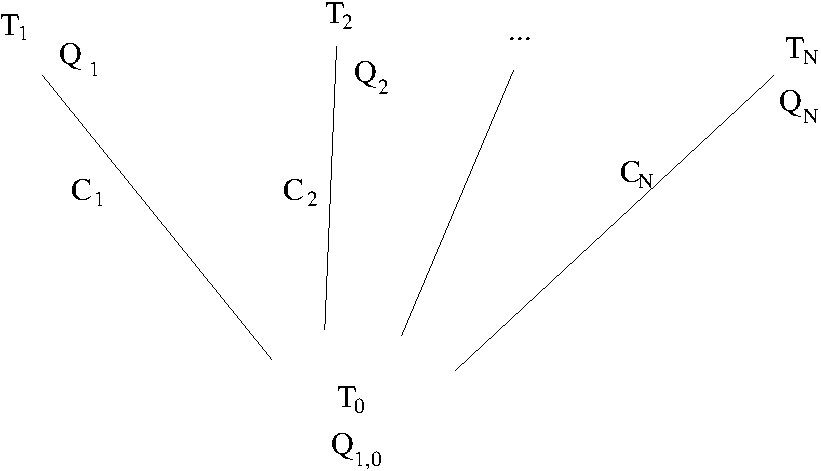
\includegraphics[scale=0.5]{immagini/fisica1/hell_machine}
\caption{macchina infernale}
\label{fig:hell_machine}
\end{figure}

passando a variabili continue:
\begin{equation}
\oint\frac{\delta Q}{T}\leq 0\quad\text{diseguaglianza di Clausius}
\label{clausius_dis}
\end{equation}
la disequazione vale per qualsiasi gas, per qualsiasi trasformazione.

Se $M$ reversibile costruisco $H'=M^{-1}+\sum_{i=1}^N C_i$, $Q$ è cambiato si segno, quindi la diseguaglianza diventa:
\[\oint\frac{\delta Q}{T}\geq0\]
Confrontando questa diseguaglianza con quella di Clausius \eqref{clausius_dis} si conclude che per una macchina reversibile:
\begin{equation}
\oint\frac{\delta Q}{T}=0
\end{equation}
Infatti considerando trasformazioni reversibili $\Delta S$ è una funzione di stato:
\[\int_i^f\frac{\delta Q}{T}=S(f)-S(i)\qquad\oint\frac{\delta Q}{T}=\int_A^A\frac{\delta Q}{T}=S(A)-S(A)=0\]

\subsection{Entropia per qualsiasi trasformazione\index{entropia! per qualsiasi trasformazione}}
Considerando un ciclo con trasformazioni irreversibili come in figura~\ref{fig:ciclo_misto}
\begin{figure}[!htbp]
\centering
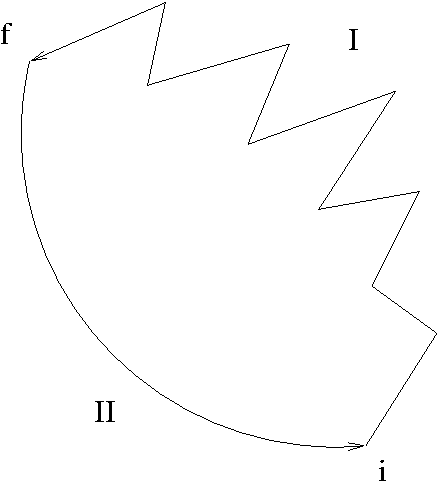
\includegraphics[scale=0.5]{immagini/fisica1/ciclo_misto}
\label{fig:ciclo_misto}
\end{figure}
dalla diseguaglianza di Clausis $\oint\frac{\delta Q}{T}\leq 0$:
\[\underbrace{\int_i^f\frac{\delta Q}{T}}_\text{irreversibile}-\underbrace{\int_i^f\frac{\delta Q}{T}}_\text{reversibile}\leq 0\]
\[\underbrace{\int_i^f\frac{\delta Q}{T}}_\text{irreversibile}\leq\underbrace{\int_i^f\frac{\delta Q}{T}}_\text{reversibile}=\Delta S\]
Per una trasformazione qualsiasi (anche irreversibile):
\[\Delta S\geq\int_i^f\frac{\delta Q}{T}\]
Nel caso sia reversibile vale l'uguaglianza.

\subsection{Entropia e secondo principio}
\[\Delta S\geq\int_i^f\frac{\delta Q}{T}\]
se consideriamo un sistema isolato $\delta Q=0$ quindi
\begin{equation}
\Delta S\geq 0 
\end{equation}
Questa equazione è equivalente al secondo principio. Se avvengono solo trasformazioni reversibili $\Delta S=0$ quindi l'entropia dell'universo non può diminuire. Le trasformazioni reversibili si dice che non lasciano traccia entropica. L'aumento dell'entropia è equivalente al secondo principio (enunciato di Kelvin o di Clausius):
\subsubsection{Macchina perfetta\index{macchina!perfetta}}

\[\Delta S_\text{sistema}=0 \qquad\text{perché ciclo}\]
\[\Delta S_\text{universo}=\Delta S_\text{sistema}+\Delta S_\text{sorgente}\]
\[\Delta S_\text{universo}=\Delta S_\text{sorgente}=\frac{Q_1}{T_1}<0\]
\[\Delta S<0\qquad \text{impossibile}\]
$Q_1$ è negativo perché lo si deve considerare dal punto di vista della sorgente per calcolare la variazione di entropia della sorgente.

\subsubsection{Frigorifero perfetto\index{frigorifero!perfetto}}


\[|Q_1|=|Q_2|=Q\]
\[\Delta S_\text{universo}=\Delta S_\text{sistema}+\Delta S_1+\Delta S_2=\frac{|Q|}{T_1}-\frac{|Q|}{T_2}=|Q|\left(\frac{1}{T_1}-\frac{1}{T_2}\right)<0\]
\[\Delta S<0\qquad \text{impossibile}\]
questo perché $T_1>T_2$; se fosse $T_2>T_1$ cioè il calore circolasse dalla sorgente calda a quella fredda $\Delta S\geq 0$ e non ci sarebbe nulla di assurdo.

\subsubsection{Secondo principio\index{secondo principio della termodinamica}\index{principio!secondo della termodinamica}}
\[\Delta S_\text{sistema isolato}\geq 0\]
L'uguaglianza solo per trasformazioni reversibili.


\subsection{Interpretazione statistica dell'entropia}
\begin{figure}[htbp]
\centering
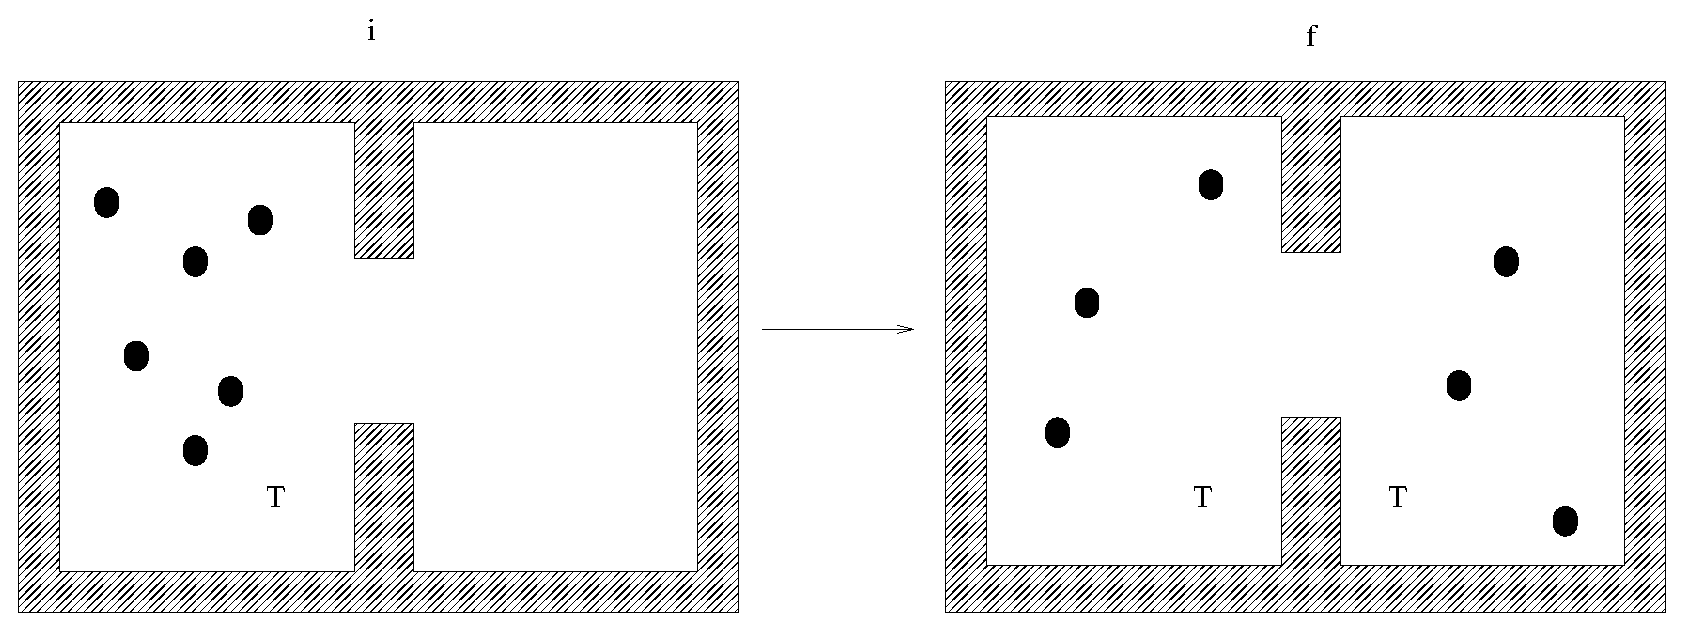
\includegraphics[scale=0.45]{immagini/fisica1/exp_Joule}
\caption{espansione di Joule.}
\end{figure}

Nell'espansione libera (o di Joule\footnote{si legge giul, non giaul (è francese!)}) si verifica sperimentalmente che la temperatura non varia. Essa è una trasformazione irreversibile spontanea. \`E isolata dall'ambiente essendo le pareti adiabatiche. Le pareti sono indeformabili, non viene compiuto lavoro. $\Delta S_\text{ambiente}=0$ $V_f=2V_i$

\[\Delta S_\text{universo}=\Delta S_\text{sistema}+\Delta S_\text{ambiente}=nR\log\frac{V_f}{V_i}=nR\log 2>0\]

\[P=\text{numero di microstati che danno luogo ad uno stato termodinamico}\]
$P$ è la probabilità che il sistema si configuri in un dato stato termodinamico a meno di un coefficiente, chiamata anche molteplicità.

$S$ è una variabile termodinamica estensiva, quindi per calcolare l'entropia del sistema si somma $S_1$ della parte sinistra e $S_2$ della parte destra. Le variabili termodinamiche come $T$, $p$ sono intensive e sommarle in questo caso non ha senso.
\begin{legge}[legge di Boltzman]
\index{Boltzmann}\index{legge!di Boltzmann}
Entropia secondo Boltzmann\index{entropia!secondo Boltzmann}:
\begin{equation}
S=k\log P
\end{equation}
\end{legge}
Diciamo che due configurazioni sono equivalenti se presentano lo stesso numero di particelle a destra e lo stesso numero di particelle a destra. L'equivalenza è logica in quanto le particelle sono indistinguibili. $P=\binom{N}{n}$ per ogni classe di equivalenza, avendo $N=6$ particelle totali:
\begin{center}
\begin{tabular}{c|c|c}
$N_S$&$N_D$&$P$\\
\hline
6&0&1\\
5&1&6\\
4&2&15\\
3&3&20\\
2&4&15\\
1&5&6\\
0&6&1\\
\end{tabular}
\end{center}
Si nota che è più probabile osservare una configurazione in cui l'entropia è aumentata (3,3) che una dove l'entropia non è aumentata. Con questo approccio non si esclude l'ipotesi che l'entropia possa diminuire, ma è estremamente improbabile, soprattutto se si considera un numero di particelle estremamente più grande.

In generale lo stato più probabile è quello con $\frac{N}{2}$ particelle a destra e a sinistra, quindi:
\[P=\binom{N}{n}=\frac{N!}{\left(\frac{N}{2}\right)!\left(\frac{N}{2}\right)!}=\frac{N!}{\left[\left(\frac{N}{2}\right)!\right]^2}\]
Stearling: $\log n!\sim n\log n-n$
\begin{align*}
\log P&=\log N!-2\log\left(\frac{N}{2}!\right)\sim N\log N-N-2\left[\frac{N}{2}\log\frac{N}{2}-\frac{N}{2}\right]=\\
&=N\log N-N-N\log\frac{N}{2}+N=N\log N-N\left(\log N-\log 2\right)\\
&=N\log 2
\end{align*}

\[S_f=k\log P=kN\log 2=nR\log 2\]
la formula è identica a quella trovata a livello macroscopico considerando la variazione di entropia dell'espansione libera come la variazione dell'entropia di una isoterma.

\begin{Es}[Esempio ghiaccio]
Ghiaccio a $T_G=\si{273.15}{\kelvin}$ di massa $m$ in acqua a $T_A=\unit{(273.15+\varepsilon)}\kelvin$
\begin{align*}
\Delta S_\text{acqua}=&S_\text{acqua}-S_\text{ghiaccio e acqua}\\
=&\int_\text{ghiaccio}^\text{acqua}\frac{\delta Q}{T}=\frac{1}{T_0}\int_\text{ghiaccio}^\text{acqua}\delta Q=\frac{Q}{T_0}=\frac{\lambda m}{T_0}>0
\end{align*}
\[\Delta S_\text{ghiaccio}=\frac{\lambda m}{T_0}\]
\[\Delta S_\text{vasca}=-\frac{\lambda m}{T_0}\]
\[\Delta S_\text{universo}=0\quad\text{perché reversibile}\]
\end{Es}
\subsection{Grafici S/T}
L'area sottesa un grafico p/V era il lavoro svolto durante la trasformazione. In un grafico S/T sarà:
\[\int_A^B T\ud S=\int_A^B\delta Q=Q\]
\subsubsection{Ciclo di Carnot\index{ciclo!di Carnot}}
\[\eta=\frac{|L|}{Q_1}=\frac{Q_1-|Q_2|}{Q_1}=\frac{\Delta S_1T_1-|\Delta S_2| T_2}{\Delta S_1 T_1}=\frac{\Delta S\Delta T}{\Delta S T_1}=\frac{T_1-T_2}{T_1}=1-\frac{T_2}{T_1}\]
Nota che: $\Delta S_1=-\Delta S_2$, ne segue che $\Delta S_\text{macchina}=0$. Ma anche \mbox{$\Delta S_\text{sorgenti}=0$} perché $\frac{Q_1}{T_1}=-\frac{Q_2}{T_2}$, quindi $\Delta S_\text{universo}=0$, infatti la trasformazione è reversibile.

L'espressione del rendimento è identica a quella trovata in precedenza.
\subsection{Generalizzazione del principio di Carnot\index{principio!di Carnot}}
Immaginiamo una macchina infernale che scambia calore con più sorgenti, con temperature comprese tra $T_{\max}$ e $T_{\min}$.
\[\sum\frac{Q_i}{T_i}=\sum\frac{Q_{a,i}}{T_i}-\sum\frac{|Q_{c,i}|}{T_i}\leq 0\]
\[\sum\frac{Q_{a,i}}{T_{\max}} \leq \sum\frac{Q_{a,i}}{T_i}\leq\sum\frac{|Q_{c,i}|}{T_i}\leq\sum\frac{|Q_{c,i}|}{T_{\min}}\]
\[\frac{\sum Q_{a,i}}{\sum|Q_{c,i}|}\leq\frac{T_{\max}}{T_{\min}}\qquad \frac{\sum |Q_{c,i}|}{\sum Q_{a,i}}\geq\frac{T_{\min}}{T_{\max}}\]
\[L+\sum Q_{a,i}-\sum|Q_{c,i}|=0\quad |L|=-L=\sum Q_{a,i}-\sum|Q_{c,i}|\]
\[\eta_M=\frac{|L|}{Q_a}=\frac{|L|}{\sum Q_{a,i}}=\frac{\sum Q_{a,i}-\sum |Q_{c,i}|}{\sum Q_{a,i}}=1-\frac{\sum|Q_{c,i}|}{\sum Q_{a,i}}\leq 1-\frac{T_{\min}}{T_{\max}}=\eta_C\]
\[\eta_M\leq\eta_C\]


\section{Scala termodinamica o assoluta\index{scala termodinamica}\index{scala assoluta}}
La scala di temperatura definita come quella del termometro a gas risulta limitata per temperature molto basse, al di sotto della quale ($\si{1}{\kelvin}$) non esiste materia allo stato gassoso. Per questo motivo viene definita la scala termodinamica. Per qualsiasi macchina reversibile (anche per uno scarafaggio che gira):
\[\eta_\text{rev}=\eta_C=1-\frac{T_2}{T_1}=1-\frac{|Q_2|}{Q_1}\]
\[\frac{\theta_2}{\theta_1}=\frac{|Q_2|}{Q_1}=\frac{T_2}{T_1}\]



\section{Riassunto trasformazioni}
\begin{center}
\begin{tabular}{p{2cm}|cccc}
&$L$&$Q$&$\Delta E$&$\Delta S$\\
\hline
Isoterma&$-nRT\log\frac{V_f}{V_0}$&$nRT\log\frac{V_f}{V_0}$&$0=nc_V\Delta T$&$nR\log\frac{V_f}{V_i}=\frac{Q}{T}$\\
Isocora&$0$&$nc_V\Delta T$&$nc_V\Delta T$&$nc_V\log\frac{T_f}{T_i}$\\
Isobara&$-p\Delta V$&$nc_p\Delta T$&$nc_V\Delta T$&$nc_p\log\frac{T_f}{T_i}$\\
Adiabatica&$nc_V\Delta T$&$0$&$nc_V\Delta T$&$0$\\
Espansione libera&$0$&$0$&$0=nc_V\Delta T$&$nR\log 2$\\
\end{tabular}
\end{center}
\index{termodinamica|)}


\chapter{Relatività speciale\index{relatività!speciale|(}\index{relatività!ristretta|see{speciale}}}
\minitoc
La relatività ristretta modifica la meccanica classica. La differenza si nota soprattutto ad alte energie ovvero ad alte velocità. Come tutte le teorie che ampliano un'altra deve rispettare il principio di corrispondenza\index{principio!di corrispondenza}, cioè deve spiegare come la relatività classica possa funzionare a basse energie, cioè come possa essere interpretata come approssimazione per basse energie.

Alla fine dell'800 si sviluppa l'elettromagnetismo, mentre la meccanica di Newton era stata applicata a tutti i campi conosciuti con estremo successo.

Bisognava far convivere le equazioni di Maxwell\index{Maxwell} con quelle di Newton.

Le leggi della meccanica sono le stesse per traslazioni uniformi, cioè sono invarianti per traslazioni. Variabili invarianti sono quelle che non cambiano per sistemi di riferimento inerziali, come l'accelerazione, la massa. Non si può esclusivamente con esperimenti di meccanica determinare se il sistema è fermo o in modo rettilineo uniforme, cioè non si possono distinguere i sistemi inerziali, quindi non esiste un sistema privilegiato.

\section{Esperimento di Michelson--Morley\index{Michelson}\index{Morley}\index{esperimento!di Michelson--Morley|(}}
\begin{figure}[htbp]
\centering
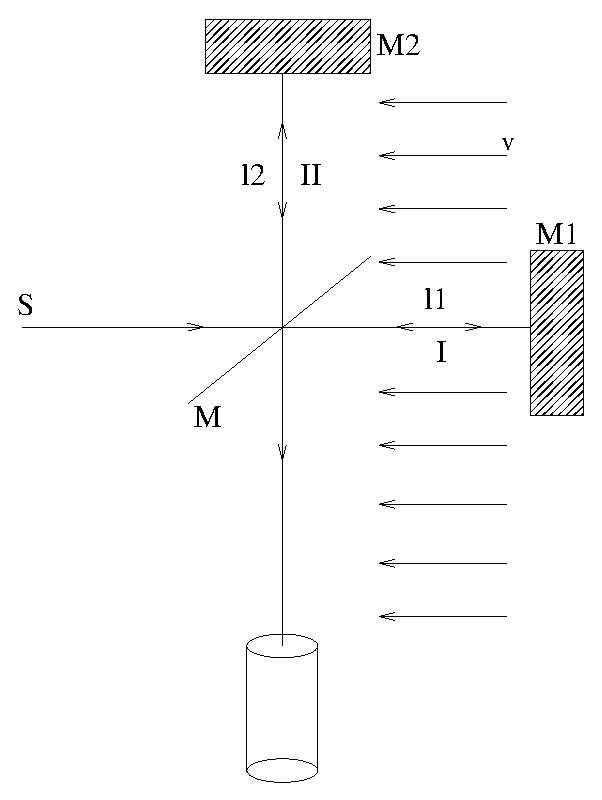
\includegraphics[scale=0.7]{immagini/fisica1/Morley}
\caption{Esperimento di Michelson--Morley.}
\end{figure}
Maxwell dice: ``$c=\frac{1}{\sqrt{\varepsilon_0\mu_0}}$'', cioè che la velocità della luce \index{velocità!della luce nel vuoto}\index{c@$c$|see{velocità della luce nel vuoto}}nel vuoto è costante e non dipende dal sistema di riferimento, contrariamente a quanto si ricava dalle trasformate di Galileo. A meno di associare quel valore $c$ ad un sistema di riferimento privilegiato si crea una spaccatura tra l'elettromagnetismo e la meccanica di Newton. Si inventa l'etere, un sistema di riferimento privilegiato che permea tutto l'universo; Michelson--Morley dimostrano che questo non può esistere.\index{etere}

Nell'esperimento la luce proviene da una sorgente $S$, viene parzialmente riflessa da uno specchio semiargentato $M$ e contemporaneamente trasmessa. La luce quindi segue due cammini: $\text{I}$ e $\text{II}$; si riflette sugli specchi $M_1$ e $M_2$ e si riunisce in un raggio unico, prima di arrivare ad un'analizzatore. Le lunghezze dei percorsi dopo lo specchio $M$, $l_1$ e $l_2$ sono circa uguali, ma non uguali se riferite alla lunghezza d'onda della luce, quindi nell'analizzatore si dovrebbe vedere una figura d'interferenza. Si suppone che l'etere sia il sistema di riferimento assoluto e che l'apparecchio si muova con velocità $v$ verso destra, quindi si può supporre che sia l'etere a spostarsi verso sinistra con velocità $v$, il ``vento d'etere''. Non si considera il percorso dalla sorgente allo specchio $M$ e dallo specchio $M$ al rivelatore, in quanto i raggi viaggiano insieme. Il tempo per andare da $M$ a $M_1$ e tornare è:
\[t_1=\frac{l_1}{c-v}+\frac{l_1}{c+v}=\frac{l_1(2c)}{c^2-v^2}=\frac{2c}{c^2}\frac{l_1}{1-\left(\frac{v}{c}\right)^2}=\frac{2l_1}{c}\frac{1}{1-\left(\frac{v}{c}\right)^2}\]
Il percorso $\text{II}$ è ortogonale al vento d'etere, per semplicità si considera il punto di vista del vento d'etere:
\begin{figure}[htbp]
\centering
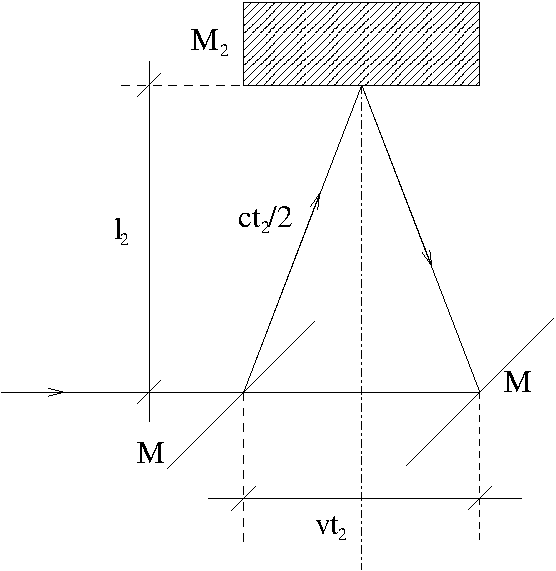
\includegraphics[scale=0.8]{immagini/fisica1/Morley2}
\caption{apparecchiatura vista dall'etere.}
\end{figure}

\parbox[]{\textwidth}{
\[s=2\sqrt{l_2^2+\left(\frac{vt_2}{2}\right)^2}=ct_2\]
\[l_2^2+\frac{v^2t_2^2}{4}=\frac{c^2t_2^2}{4}\qquad l_2^2=\frac{1}{4}\left(c^2-v^2\right)t_2^2\]
\[t_2=\frac{2l_2}{\sqrt{c^2-v^2}}=\frac{2l_2}{c}\frac{1}{\sqrt{1-\left(\frac{v}{c}\right)^2}}\]
}
La differenza di tempo dei due cammini è:
\[\Delta t=t_2-t_1=\frac{2}{c}\left\{\frac{l_2}{\sqrt{1-\left(\frac{v}{c}\right)^2}}-\frac{l_1}{1-\left(\frac{v}{c}\right)^2}\right\}\]
si osserva quindi una figura di interferenza. Se l'apparecchiatura viene ruotata di $90^\circ$ $l_1$ e $l_2$ si invertono:
\[\Delta t'={t_2}'-{t_1}'=\frac{2}{c}\left\{\frac{l_2}{{1-\left(\frac{v}{c}\right)^2}}-\frac{l_1}{\sqrt{1-\left(\frac{v}{c}\right)^2}}\right\}\]

\parbox[]{\textwidth}{
Si dovrebbe osservare una figura di interferenza diversa:
\begin{align*}
\Delta=&\Delta t'-\Delta t=\frac{2}{c}\left\{\frac{l_1+l_2}{{1-\left(\frac{v}{c}\right)^2}}-\frac{l_1+l_2}{\sqrt{1-\left(\frac{v}{c}\right)^2}}\right\}\\
=&\frac{2}{c}(l_1+l_2)\left\{1+\left(\frac{v}{c}\right)^2+\ldots-\left(1+\frac{1}{2}\left(\frac{v}{c}\right)^2\right)\right\}\\
\simeq&\frac{2}{c}(l_1+l_2)\frac{1}{2}\left(\frac{v}{c}\right)^2=\frac{l_1+l_2}{c}\left(\frac{v}{c}\right)^2\end{align*}
}
Con più riflessioni si riesce ad avere $l_1+l_2=\si{20}{\metre}$, considerando il Sole come riferimento assoluto si ha $v=\si{30}{\kilo\meter\per\second}$ e $\lambda=\si{500E-9}{\metre}$.
Il numero di frange che scorrono dovrebbe essere:
\[\Delta N=\frac{\Delta}{T}=\frac{l_1+l_2}{\lambda}\left(\frac{v}{c}\right)^2\simeq 0.4\]
La sensibilità dello strumento era $\Delta N=0.01$. Se ci fosse stato l'etere con quella velocità sarebbe stato osservato. La ricerca dell'etere ripetuta in più mesi dell'anno, di giorno e di notte, usando luce solare, stellare ed artificiale, con dispositivi diversi, usando bracci diversi, telescopi o osservando fenomeni elettrici diede risultato negativo. Nel 1907 Nobel per Michelson.
\index{esperimento!di Michelson--Morley|)}
\section{Postulati di Einstein\index{Einstein!postulati di}\index{postulato!di Einstein}}
\begin{post}[Primo postulato della relatività ristretta]
Tutte le leggi fisiche sono invarianti per traslazioni uniformi
\end{post}
\begin{post}[Secondo postulato della relatività ristretta]
La velocità della luce nel vuoto è uguale in tutti i sistemi di riferimento
\end{post}

I postulati di Einstein sono ampiamente verificati sperimentalmente. L'esperimento di Michelson--Morley verifica il primo postulato di Einstein. Per il secondo postulato si può considerare il seguente esperimento: il Sole ruota rispetto al suo asse, quindi la sorgente di luce si muove. Si misura la differenza di velocità dei raggi di luce provenienti da due estremi dell'equatore del sole. Le velocità misurate sono abbastanza simili da verificare il secondo postulato.

\subsection{Simultaneità}

\begin{figure}[htbp]
   \centering
   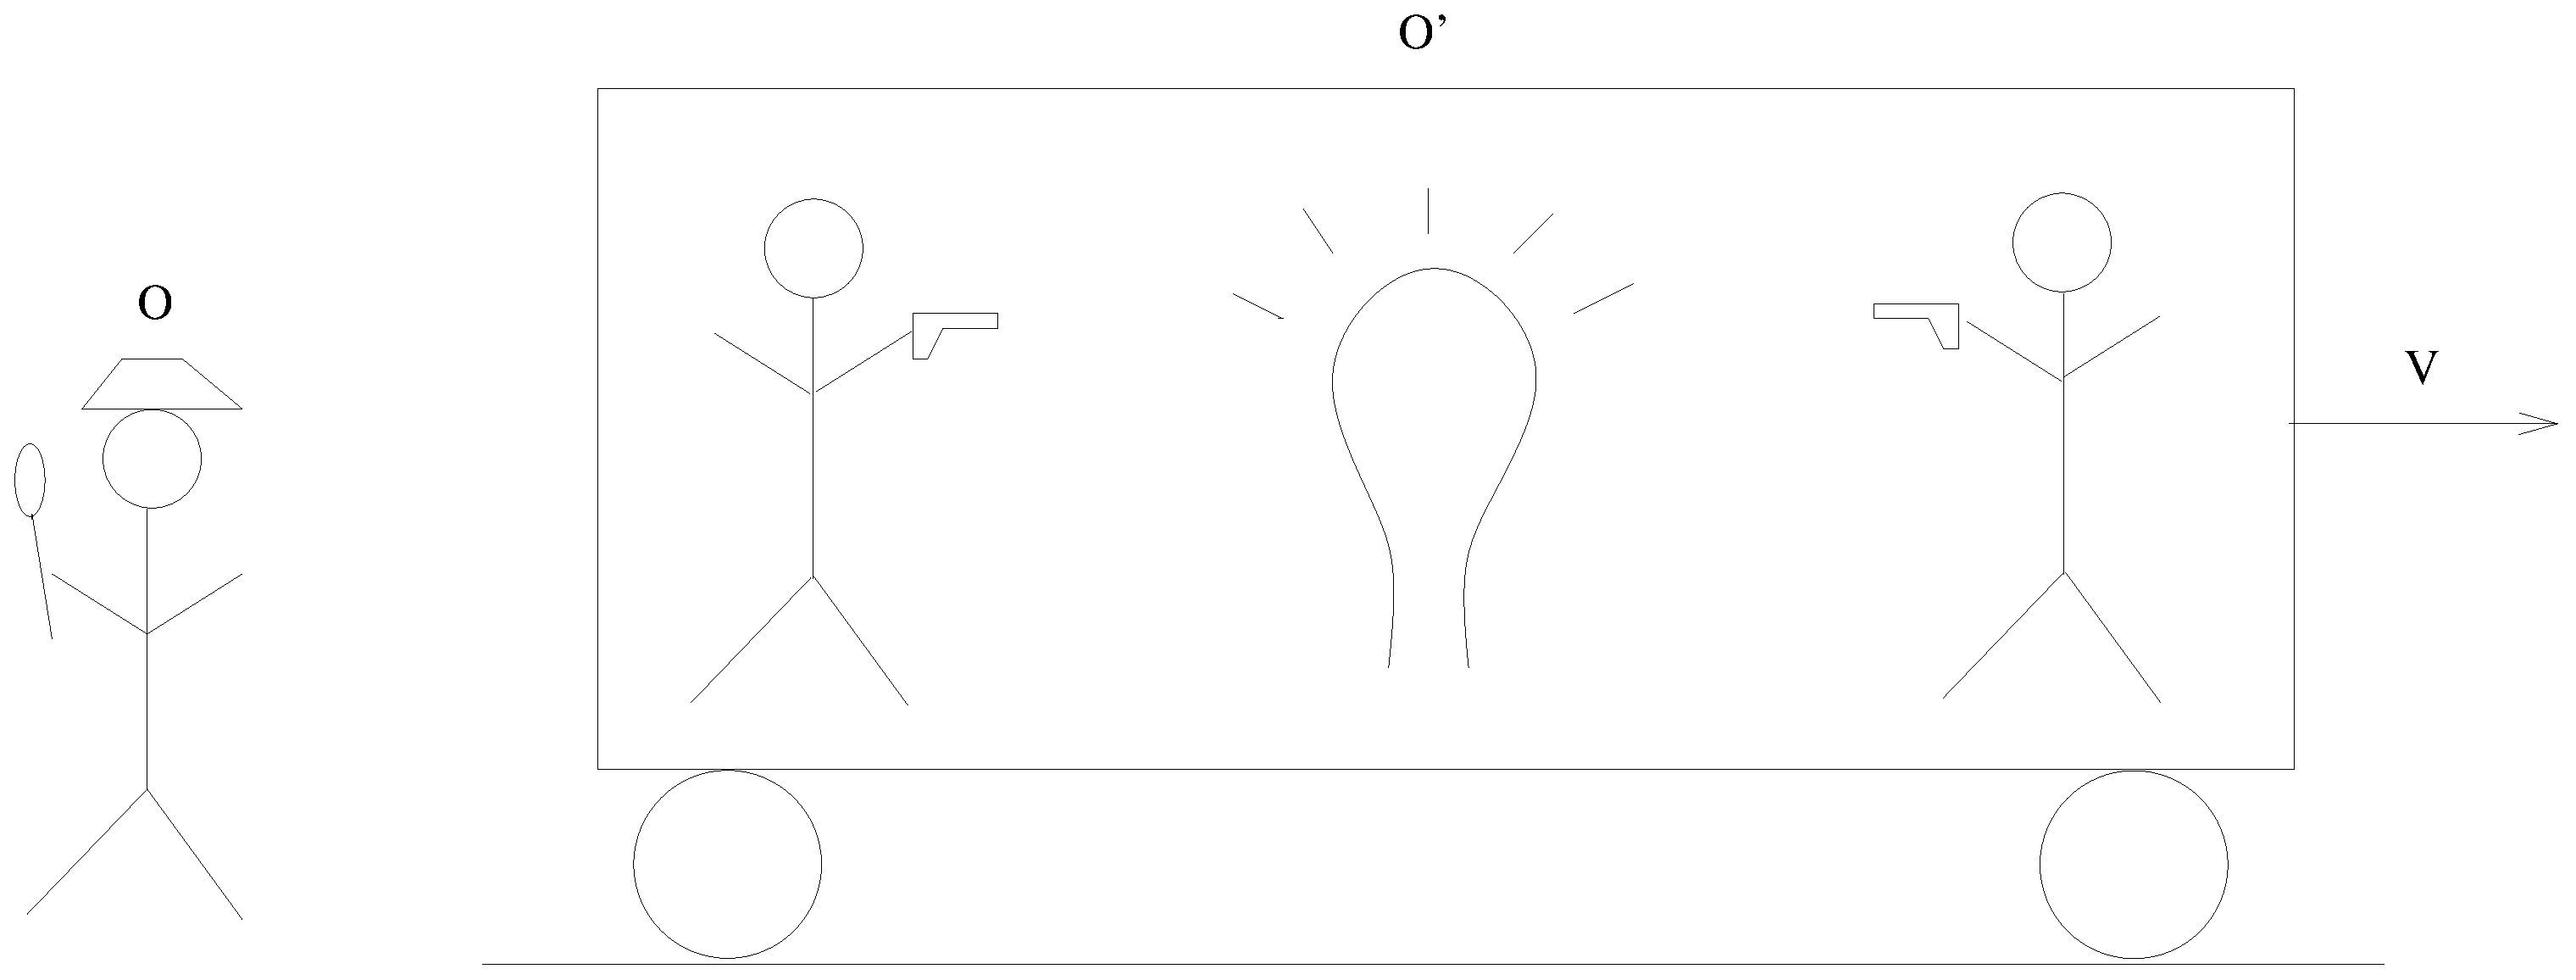
\includegraphics[scale=0.2]{immagini/fisica1/pistoleri}
   \caption{pistoleri relativistici.}
   \label{pistoleri}
\end{figure}


I due pistoleri (Fig.\@ \ref{pistoleri}) sparano quando la luce gli raggiunge. Essi sono in un sistema solidale con la luce e quindi vedono contemporaneamente la luce della lampadina. Per il capostazione ``fermo'' invece è il pistolero di sinistra ad essere investito per prima dalla luce, quindi il pistolero a destra muore, mentre quello di sinistra no. Gli eventi simultanei per $O'$ non sono tali per $O$, bisogna rivedere il concetto di tempo assoluto.

\section{Trasformate di Lorentz\index{trasformate!di Lorentz|(}\index{trasformazioni!di Lorentz|(}\index{Lorentz}}
Le trasformate i Lorentz sostituiscono le trasformate di Galileo della meccanica classica. Per velocità basse rispetto a quelle della luce le trasformate di Lorentz tendono a quelle di Galileo.
La funzione che trasforma le coordinate di un sistema di riferimento a quelle di un altro deve essere lineare, in quanto lo spazio è omogeneo. Immaginiamo che l'applicazione non sia omogenea, e quindi non lineare, per esempio: $x'=kx^2$. Se mettiamo una sbarra tra $0$ e $1$ questa misura $\Delta x=1-0=1$, nel nuovo sistema di riferimento misura: $k\cdot 1^2-k\cdot 0^2=k$. Se ora mettiamo la sbarra tra $2$ e $1$ nel primo sistema di riferimento misurerà ancora $1$, mentre nel secondo $k(2^2-1^2)=3k$ ovvero spostando la sbarra nel secondo sistema di riferimento la sua lunghezza cambia: assurdo per l'ipotesi di omogeneità dello spazio; inoltre l'applicazione deve essere anche additiva, perché la lunghezza di due sbarre affiancate deve essere la somma dell'unica sbarra avente lunghezza uguale nel primo sistema di riferimento alla somma delle lunghezze delle due sbarre nel primo sistema di riferimento. Consideriamo il sistema di riferimento $Oxy$ fermo e $O'x'y'$ che si muove rispetto ad $O$ di moto rettilineo uniforme con velocità di trascinamento $u$ nella direzione dell'asse $x$ crescente. L'applicazione è lineare, quindi (in due dimensioni spaziali), in generale:
\[\left\{
\begin{array}{l}
x'=\lambda_{11}x+\lambda_{12}y+\lambda_{14}t\\
y'=\lambda_{21}x+\lambda_{22}y+\lambda_{24}t\\
t'=\lambda_{41}x+\lambda_{42}y+\lambda_{44}t\\\end{array}\right.
\]
``Solo'' 9 incognite. Ipotesi aggiuntive:
\begin{itemize}
\item[-] al tempo $t=t'=0$ gli orologi coincidono e anche i sistemi di riferimento $O\equiv O'$, in particolare per $t=0$ e $x=0$ segue $x'=0$ cioè
\[x'=\lambda_{11}x+\lambda_{12}y+\lambda_{14}t\]
\[0=\lambda_{11}\cdot 0+\lambda_{12}y+\lambda_{14}\cdot 0\]
\[\lambda_{12}=0\]
\item[-] come sopra:
\[t'=\lambda_{41}x+\lambda_{42}y+\lambda_{44}t\]
\[0=0+\lambda_{42}y+0\]
\[\lambda_{42}=0\]
\item[-] la traslazione del sistema in moto è orizzontale, quindi $y'=0\Leftrightarrow y=0$ sempre.
\[\lambda_{21}=0\]
\[\lambda_{24}=0\]

\end{itemize}

Se mettiamo una sbarra verticalmente con un estremo in $O'$, questo misura che la lunghezza è $1$. La sbarra si muove con $O'$ e quindi questa è la lunghezza a riposo. Questa lunghezza a riposo dovrà essere uguale anche se è osservata da $O$. Mettiamo la sbarra ferma rispetto ad $O'$, quindi $O$ vede una lunghezza:
\[y=\frac{1}{\lambda_{22}}\]
mettiamo ora la sbarra ferma rispetto a $O$, $O'$ vede una lunghezza:
\[y'=\lambda_{22}\]
Le due situazioni sono simmetriche e quindi non esistendo un sistema privilegiato le due grandezze devono essere uguali:
\[\lambda_{22}=\frac{1}{\lambda_{22}}\qquad\lambda^2_{22}=1\]
Si scarta la soluzione negativa, in quanto si vuole che gli assi abbiano lo stesso verso.


\parbox[]{\textwidth}{
Seguiamo il moto dell'origine del sistema $O'$. Qui, per ogni istante:
\[x'=0\]
Per $O$ lo stesso moto è descritto da:
\[x=ut\qquad x-ut=0\]
Ci si aspetta allora un'equazione del tipo
\[x'=\lambda(x-ut)\]
}

A $t=0$, $O\equiv O'$, $t=t'$ scatta un'onda luminosa dalle origini, questa ha un fronte sferico con raggio $R$ e per il secondo principio di Einstein ha velocità $c$ uguale in tutti e due i sistemi. Il sistema $O'$ sta arrivando da sinistra, passa in coincidenza con $O$, si sincronizzano gli orologi e parte il fronte d'onda. I due osservatori osservano un fronte d'onda che ha centro nei propri sistemi di riferimento, anche se non sono più coincidenti:
\[x^2+y^2+z^2=R^2=(ct)^2\]
\[x'^2+y'^2+z'^2=R'^2=(ct')^2\]
\[x^2+y^2+z^2-ct^2=0=x'^2+y'^2+z'^2-(ct')^2\]
\[x^2-c^2t^2=x'^2-c^2t'^2=\lambda^2(x-ut)^2-c^2(\lambda_{41}x+\lambda_{44}t)^2=\]
\[=\lambda^2x^2+\lambda^2 u^2t^2-2\lambda^2 xut-c^2\lambda_{41}^2x^2-c^2\lambda_{44}^2t^2-2c^2\lambda_{41} x\lambda_{44} t\]
Risolvendo in $\lambda^2$, $\lambda_{41}^2$ e $\lambda_{44}^2$ si ottiene un sistema di tre incognite e tre equazioni:
\[\left\{
\begin{array}{l}
1=\lambda^2-c^2\lambda_{41}^2\\
-c^2=\lambda^2u^2-c^2\lambda_{44}^2\\
0=-2\lambda^2u-2c^2\lambda_{41}\lambda_{44}\\
\end{array}
\right.\quad \left\{
\begin{array}{l}
\lambda_{41}^2=\frac{\lambda^2-1}{c^2}\\
\lambda_{44}^2=\frac{c^2+\lambda^2u^2}{c^2}\\
-\lambda^2u=c^2\lambda_{41}\lambda_{44}\\

\end{array}\right.\]
Ci ricordiamo dell'ultima espressione che $\lambda_{41}\lambda_{44}<0$
\[\lambda^4u^2=c^4\lambda_{41}^2\lambda_{44}^2=c^4\frac{\lambda^2-1}{c^2}\frac{c^2+\lambda^2u^2}{c^2}=\]
\[=(\lambda^2-1)(c^2+\lambda^2u^2)=-c^2-\lambda^2u+\lambda^2c^2+\lambda^4u^2\]
\[0=-c^2-\lambda^2u^2+\lambda^2c^2\]
\[\lambda^2=\frac{c^2}{c^2-u^2}=\frac{1}{1+\frac{u^2}{c^2}}\]
\[\lambda=\dfrac{1}{\sqrt{1-\left(\dfrac{u}{c}\right)^2}}=\dfrac{1}{\sqrt{1-\beta^2}}=\gamma\]
\[\lambda_{41}^2=\frac{\lambda^2-1}{c^2}=\frac{\beta^2}{c^2(1-\beta^2)}\]
\[\lambda_{41}=\pm\frac{\beta}{c\sqrt{1-\beta^2}}\]
\[\lambda_{44}^2=\frac{c^2+\lambda^2u^2}{c^2}=\frac{1}{1-\beta^2}\]
\[\lambda_{44}=\pm\frac{1}{\sqrt{1-\beta^2}}\]
Diamo segno positivo a $\lambda_{44}$ e negativo a $\lambda_{41}$, in quanto se consideriamo un istante molto prossimo al momento della partenza allora $x\rightarrow 0$, $t'$ deve essere positivo (il tempo scorre nello stesso verso) e quindi $\lambda_{44}>0$.
\subsection{Trasformate di Lorentz e Galileo}
Se $u\ll c$, cioè se $\beta\rightarrow 0$ $\Rightarrow$ Lorentz $\rightarrow$ ``buon'' Galileo e il tempo assoluto.
\[\left\{
\begin{array}{l}
x^\prime=\dfrac{x-ut}{\sqrt{1-\beta^2}}\\
y^\prime=y\\
z^\prime=z\\
t^\prime=\dfrac{t-\frac{\beta}{c}x}{\sqrt{1-\beta^2}}
\end{array}\right.
\quad \stackrel{\beta\rightarrow 0}{\longrightarrow} \quad
\left\{
\begin{array}{l}
x^\prime=x-ut\\
y'=y\\
z'=z\\
t'=t\\
\end{array}\right.\]
\index{trasformate!di Lorentz|)} \index{trasformazioni!di Lorentz|)}
\section{Contrazione delle lunghezze\index{contrazione delle lunghezze}}
\begin{figure}[htbp]
   \centering
   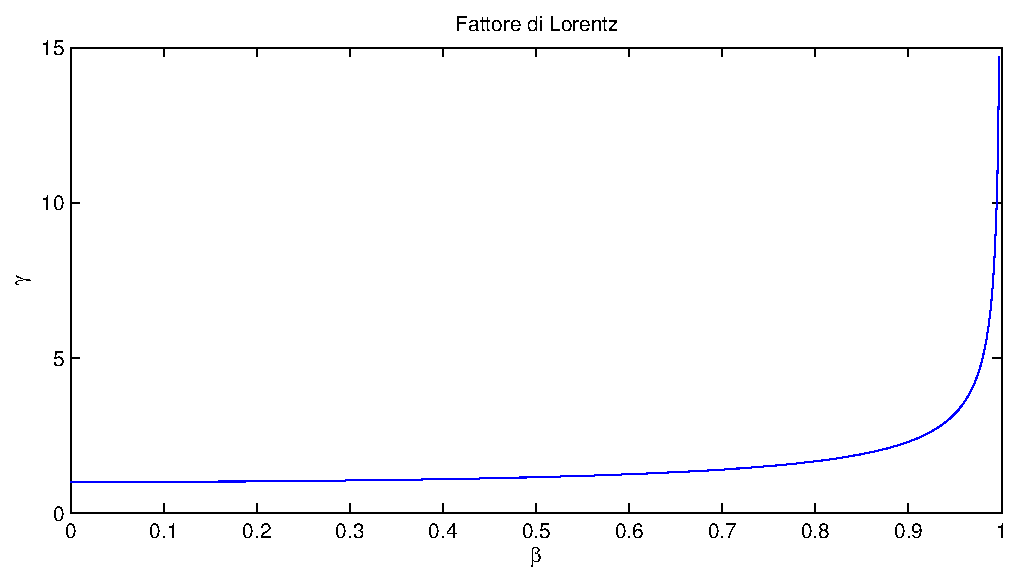
\includegraphics[scale=0.5]{immagini/fisica1/beta_gamma}
   \caption{Variazione di $\gamma$ in funzione di $\beta$.}
\end{figure}
Consideriamo spazi nello stesso tempo. Posizioniamo un'asta con estremi $A$ e $B$ ferma rispetto ad $O'$, sistema di riferimento inerziale con velocità $u$ rispetto ad $O$.
$O$ misura nello stesso istante le posizione di $A$ e di $B$, quindi $t_A\equiv t_B$:
\[\left\{
\begin{array}{l}
x'_A=\frac{x_A-ut_A}{\sqrt{1-\beta^2}}\\
x'_B=\frac{x_B-ut_B}{\sqrt{1-\beta^2}}\\
\end{array}
\right.\]
\begin{align*}
l'&=x'_B-x'_A=\frac{x_B-x_A-ut_B+ut_A}{\sqrt{1-\beta^2}}=\frac{x_B-x_A-u(t_B-t_A)}{\sqrt{1-\beta^2}}=\frac{x_B-x_A}{\sqrt{1-\beta^2}}\\
&=\gamma l
\end{align*}
\begin{equation}
l=\frac{l'}{\gamma}
\end{equation}
Considerando che $0<\beta<1\Rightarrow\gamma>1$ si ha che $l<l'$, cioè $O$ osserva un oggetto in moto contratto.

\section{Dilatazione dei tempi\index{dilatazione dei tempi}}
Consideriamo eventi osservati da $O'$ nello stesso spazio ($x'_A\equiv x'_B$) a distanza di tempo $\tau'=t'_B-t'_A$.
\[t'=\gamma\left(t-\frac{\beta}{c}x\right)\]
Per simmetria posso dire direttamente che:
\[t=\gamma\left(t'+\frac{\beta}{c}x'\right)\]
\[t_A=\gamma\left(t'_A+\frac{\beta}{c}x'_A\right)\]
\[t_B=\gamma\left(t'_B+\frac{\beta}{c}x'_B\right)\]
\begin{equation}
\tau=t_B-t_A=\gamma\left(t'_B-t'_A+\frac{\beta}{c}\left(x'_B-x'_A\right)\right)=\gamma\left(t'_B-t'_A\right)=\gamma\tau'
\end{equation}
Ancora, essendo $\gamma>1$ si ha che $\tau>\tau'$ cioè $O$ vede l'evento più lentamente di $O'$.

\begin{Es}[produzione e decadimento di mesoni $\pi^+$]
Un protone colpisce un altro protone fermo:
\[p+p\rightarrow p+n+\pi^+\]
Il mesone decade:
\[\pi^+ \rightarrow \mu ^+ + \nu\]

Un omino cavalca il mesone $\pi^+$ e osserva un tempo di vita media $\tau'=\si{1.88E-8}{\second}$. Il mesone ha rispetto al laboratorio $\beta=0.99$. Il laboratorio dalla distanza percorsa dal mesone calcola una vita media diversa:
\[\tau=\gamma\tau'=\frac{\tau'}{\sqrt{1-\beta^2}}\simeq 7.1\tau'=\si{1.3E-7}{\second} \]
La distanza percorsa dal mesone, prima di decadere, osservata dal laboratorio è quindi:
\[d=\tau u=\tau \beta c\simeq \si{39}{\metre} \]
\end{Es}

\section{Composizione delle velocità\index{composizione delle velocità!relativistiche}}
La velocità rimane sempre la derivata del vettore posizione: $v_x=\frac{\ud x}{\ud t}$.
\begin{equation}
v'_{x'}=\frac{\ud x'}{\ud t'}=\frac{\ud x'}{\ud t}\frac{\ud t}{\ud t'}=\frac{\ud x'}{\ud t}\dfrac{1}{\frac{\ud t'}{\ud t}}=\gamma\left(\frac{\ud x}{\ud t}-u\right)\dfrac{1}{\gamma\left(1-\dfrac{\beta}{c}\dfrac{\ud x}{\ud t}\right)}=\dfrac{v_x-u}{1-\dfrac{\beta}{c}v_x}
\end{equation}
\begin{equation}
v'_{y'}=\frac{\ud y'}{\ud t'}=\frac{\ud y}{\ud t'}=\frac{\ud y}{\ud t}\frac{\ud t}{\ud t'}=v_y\frac{1}{\frac{\ud t'}{\ud t}}=\dfrac{v_y}{\gamma\left(1-\dfrac{\beta}{c}\dfrac{\ud x}{\ud t}\right)}=\dfrac{v_y\sqrt{1-\beta^2}}{1-\dfrac{\beta}{c}v_x}
\end{equation}
Un'analoga equazione vale per $v'_{z'}$ essendo come $v'_{y'}$ una velocità trasversa rispetto ad $u$.
\[\lim_{\beta\rightarrow 0}v'_{x'}=v_x-u\qquad \lim_{\beta\rightarrow 0} v'_{y'}=v_y\]
cioè la composizione delle velocità secondo Galileo.

\begin{Es}[decadimento $\pi^0$]
$\pi^0$ decade con un decadimento elettromagnetico del tipo:
\[\pi^0\rightarrow \gamma\gamma\]
Per la conservazione della quantità di moto i due fotoni devono avere velocità opposte, $c$ misurate sia dal sistema del laboratorio ($O$) sia dal sistema in moto con il $\pi^0$, $O'$. Supponiamo che i fotoni si propaghino secondo l'asse $x$ e che il mesone si muovesse alla velocità $u$ verso destra rispetto ad $O$. Per Einstein la velocità dei due fotoni vista da $O$ e da $O'$ è uguale.
Per il fotone che va a destra:
\[v_x=\frac{v'_{x'}+u}{1+\frac{\beta}{c}v'_{x'}}=\frac{c+u}{1+\frac{u}{c^2}c}=c\]
Per l'altro:
\[v_x=\frac{-c+u}{1-\frac{u}{c^2}(-c)}=-c\]
\end{Es}
\section{Massa\index{massa!relativistica}}
Dalla conservazione della quantità di moto ricaviamo la massa relativistica. Siano $O$ e $O'$ due osservatori dotati di due pistole identiche con proiettili identici, cioè con stesse masse a riposo. $O'$ si muove verso destra rispetto ad $O$ con velocità costante  $\ve u$. Gli assi $x$ e $x'$ non coincidono, sono sfasati, ma questo conta poco perché considerando le velocità, cioè derivando, il problema scompare. $O'$ spara in direzione di $O$ cioè nel verso delle $y$ decrescenti. $O$ vede il suo proiettile con velocità\marginpar{\begin{small}tratto da \cite{modern}\end{small}}:
\[\dot y'_{O'}=-U\qquad\dot{x'}_{O'}=0\]
$O$ vede il proiettile di $O'$ con velocità:
\[\dot y_{O'}=\frac{\dot y'_{O'}\sqrt{1-\beta^2}}{1-\frac{\beta}{c}\dot x'_{O'}}=-\sqrt{1-\frac{u^2}{c^2}}U\]
$O$ spara a $O'$ nel verso delle $y$ crescenti e misura la velocità del proiettile:
\[\dot y_{O}=U\qquad \dot x_{O}=0\]
e $O'$ vede il proiettile di $O$ con:
\[\dot y'_{O}=\sqrt{1-\frac{u^2}{c^2}}U\]
la quantità di moto si deve conservare quindi $O$ vede:
\[m_{O}U+m_{O'}\dot y_{O'}=0\]
\[m_{O'}=\frac{m_OU}{\sqrt{1-\frac{u^2}{c^2}}}U=\frac{m_O}{\sqrt{1-\frac{u^2}{c^2}}}\]
Considerando $O$ fermo:
\[m_{O}=m_0=\text{massa a riposo}\]
\[m=\frac{m_0}{\sqrt{1-\beta^2}}=\gamma m_0\]
\[\beta\rightarrow 1\Rightarrow m\rightarrow +\infty\]
\section{Quantità di moto\index{quantità di moto!relativistica}}
\[p=mv=\frac{m_0}{\sqrt{1-\beta^2}}\beta c=\gamma m_0 v\]
$\beta$ della particella. Con questa nuova definizione di quantità di moto essa si conserva ancora, anche in contesto relativistico.
\[\beta\rightarrow 1\Rightarrow p\rightarrow +\infty\]

\begin{Es}[quantità di moto classica vs relativistica]
\begin{figure}[htbp]
   \centering
   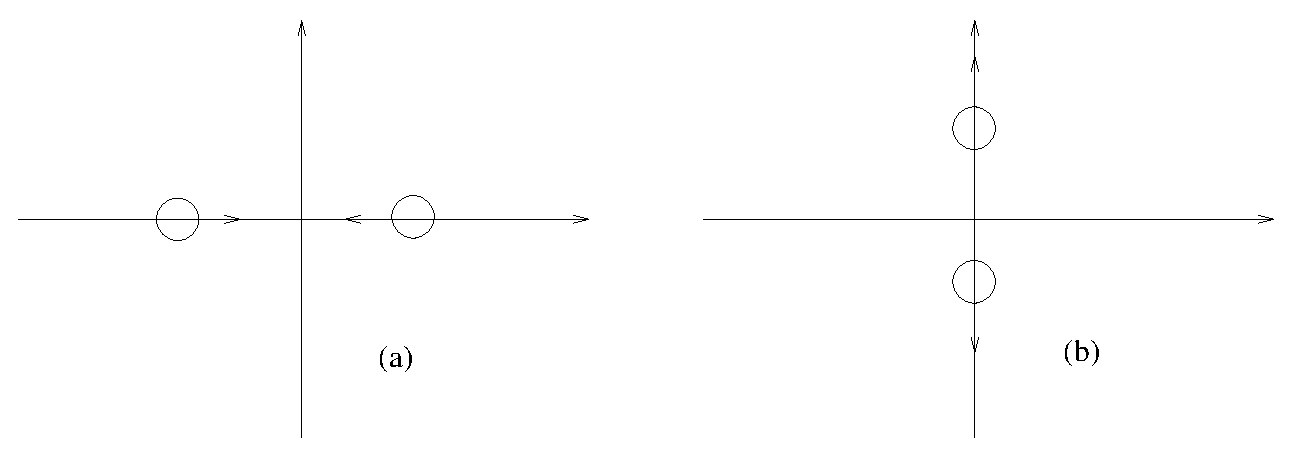
\includegraphics[scale=0.5]{immagini/fisica1/Q_rel1}
   \caption{(a) prima dell'urto; (b) dopo l'urto.}
\end{figure}
Urto frontale tra due particelle con stessa massa e velocità, sull'asse $x$. Dopo l'urto le particelle possono andare su qualunque direzione, ipotizziamo quella verticale. La quantità di moto si conserva, infatti all'inizio:
\[p_x=mv_x-mv_x=0\qquad p_y=mv_y-mv_y=0\]
e dopo l'urto:
\[p_x=mv_x-mv_x=0\qquad p_y=mv_y-mv_y=0\]
Quindi sembra che la conservazione della quantità di moto classica funzioni. Cambiamo sistema di riferimento, consideriamo quello solidale con la seconda particella. Essa prima dell'urto si muove con velocità $u=v$ verso sinistra. Utilizzando le composizioni delle velocità relativistiche:
\begin{figure}[htbp]
   \centering
   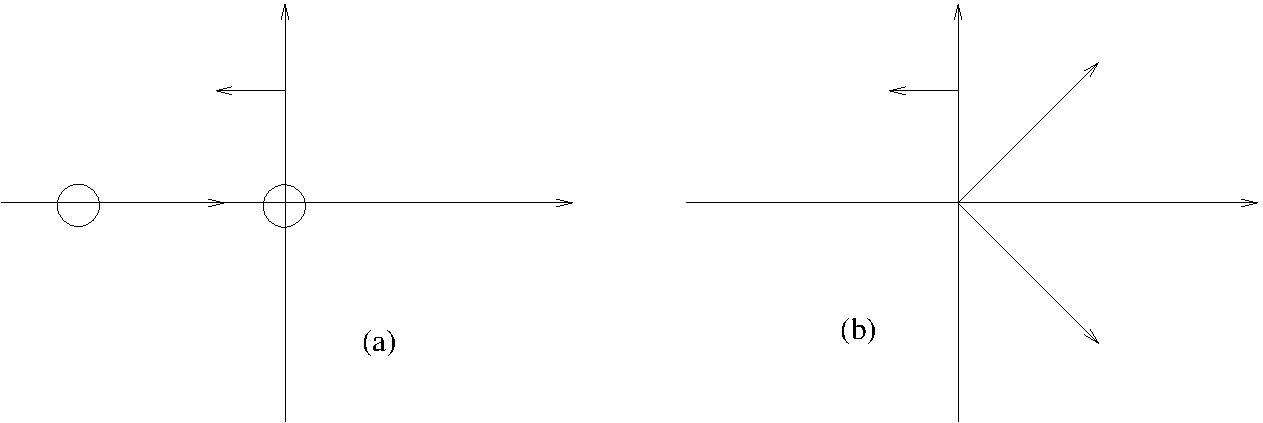
\includegraphics[scale=0.5]{immagini/fisica1/Q_rel2}
   \caption{(a) prima dell'urto; (b) dopo l'urto.}
\end{figure}

\[\left\{
\begin{array}{l}
p'_{x'}=p'_{x'_1}=\dfrac{v+v}{1+\dfrac{v^2}{c^2}}m=\dfrac{2v}{\dfrac{c^2+v^2}{c^2}}m=2mu\dfrac{1}{1+\beta^2}\\
p'_{y'}=0\\
\end{array}
\right. \]
\[\left\{
\begin{array}{l}
p'_{x'}=2mv'_{x'}=2mu\\
p'_{y'}=0\\
\end{array}
\right. \]
La quantità di moto fallisce. Bisogna considerare la correzione della massa.
\end{Es}
\section{Energia Relativistica\index{energia!relativistica}}
\label{energia_cinetica_relativistica}
\subsection{Teorema lavoro--energia\index{teorema!lavoro--energia!relativistico}}
\begin{figure}[htbp]
   \centering
   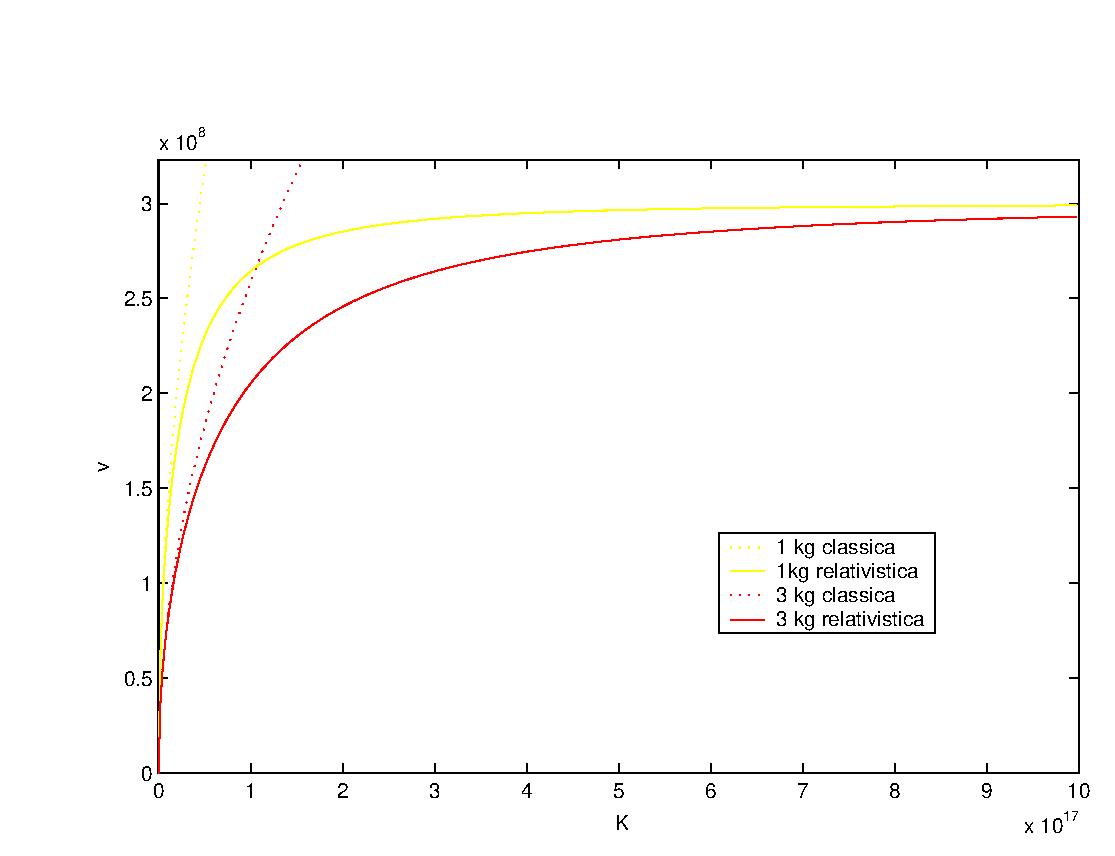
\includegraphics[scale=0.6]{immagini/fisica1/V_K}
   \caption{Velocità in funzione dell'energia cinetica con diverse masse.}
\end{figure}
Per far funzionare il teorema $L=\Delta K$ bisogna cambiare la definizione di energia cinetica.\index{energia!cinetica!relativistica}
\[m=\frac{m_0}{\sqrt{1-\beta^2}}\]
\[m^2(1-\beta^2)=m_0^2\quad m^2c^2-m^2v^2=m_0^2c^2\]
\[2mc^2\ud m-2mv^2\ud m-2m^2v\ud v=0\]
\[c^2\ud m=v^2\ud m+mv\ud v\]
Considerando solo una forza diretta come l'asse $x$:
\[L=\int_A^B \ve F\ud \ve x=\int\frac{\ud \ve p}{\ud t}\ud \ve x=\int\ud \ve p\,\frac{\ud\ve x}{\ud t}=\int \ve v\ud \ve p=\int \ve v\ud(m\ve v)=\Delta K=\]
\[=\!\int(\ud m\ve v+m\ud\ve v)\ve v=\!\!\int\!(\ud mv^2+mv\ud v)=c^2\!\!\!\int_{v_A}^{v_B}\!\!\!\!\ud m=\left(m\left(v_B\right)-m\left(v_A\right)\right)c^2\]
Se $K(0)=0$ in accordo con quella classica:
\[K(B)=K(B)-K(0)=\Delta K=(m_B-m_0)c^2\quad K=mc^2-m_0c^2\]
\[\underbrace{m_0c^2}_{\text{energia a riposo}}+\underbrace{K}_{\text{energia cinetica}}=\underbrace{mc^2}_{\text{energia totale}}\]
\[E=mc^2\qquad \Delta E=\Delta K=L\]
\[K=mc^2-m_0c^2=\frac{m_0c^2}{\sqrt{1-\beta^2}}-m_0c^2=m_0c^2\left(\frac{1}{\sqrt{1-\beta^2}}-1\right)=m_0c^2\left(\gamma-1\right)\]
\subsection{Energia cinetica classica}
\[v\ll c\qquad m_0c^2\left(1+\frac{1}{2}\beta^2+\ldots-1\right)=\frac{1}{2}m_0\beta^2c^2=\frac{1}{2}m_0v^2\]
\subsection{Urti ed energia}
\[E=m_0c^2+K=mc^2\]
\begin{figure}[htbp]
   \centering
   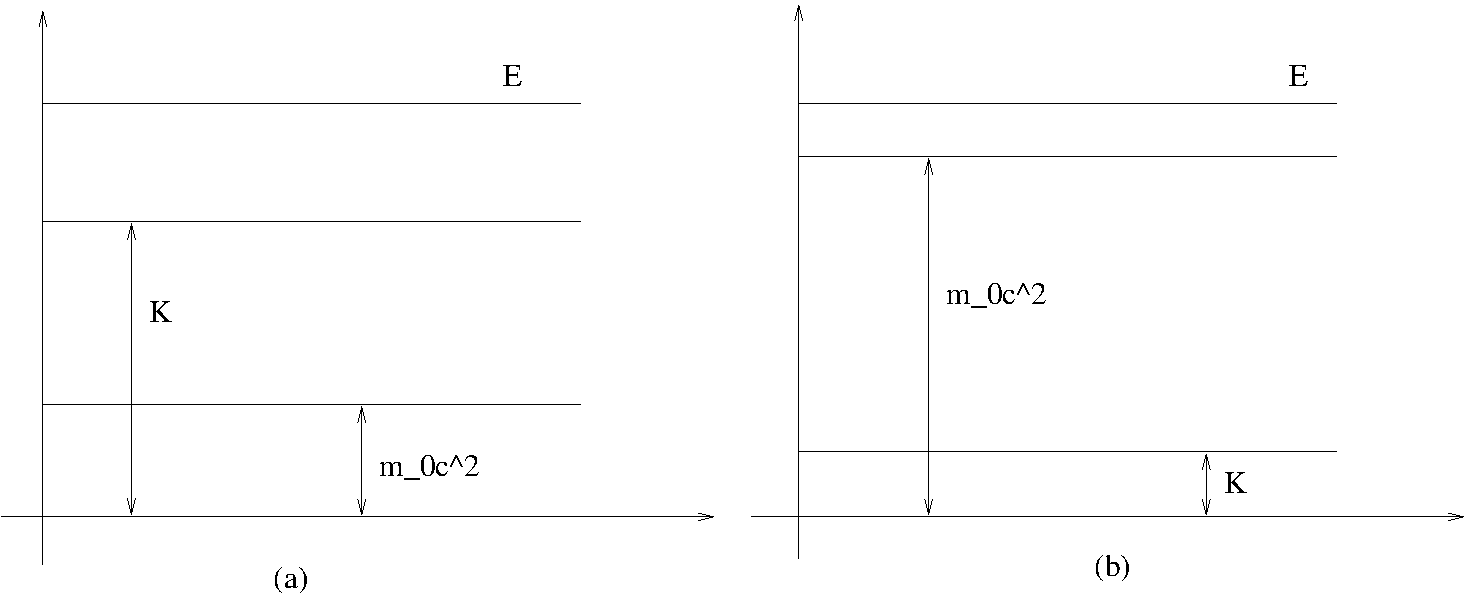
\includegraphics[scale=0.5]{immagini/fisica1/urto_rel}
   \caption{(a) prima dell'urto; (b) dopo l'urto.}
\end{figure}
La massa durante l'urto può aumentare, si creano nuove particelle. Non basta avere molta energia per creare nuove particelle, ma bisogna concentrarla.

\subsection{Conservazione dell'energia}
In meccanica classica il teorema della conservazione dell'energia diceva che l'energia totale si conservava:
\[K+U=E=\const\]
L'energia potenziale ha sempre la stessa definizione, il lavoro è definito come variazione dell'energia totale ($mc^2$):
\[\int_{r_1}^{r_2}\ve F\cdot \ud\ve r=U(\ve r_1)-U(\ve r_2)=\int_{r_1}^{r_2}\ud K=m_{r_2}c^2-m_{r_1}c^2\]
\[m_{r_1}c^2+U(r_1)=m_{r_2}c^2+U(r_2)\]
\[mc^2+U=\const\]

\section{Quantità di moto ed energia\index{quantità di moto!relativistica}\index{energia!relativistica}}
\[\left\{
\begin{array}{l}
E=mc^2=\dfrac{m_0}{\sqrt{1-\beta^2}}c^2\\
p=\dfrac{m_0}{\sqrt{1-\beta^2}}\beta c\\
\end{array}\right.
\quad\Rightarrow\quad
\dfrac{p}{E}=\dfrac{\beta}{c}
\quad\Rightarrow\quad\beta E=pc
\]
\[E^2=\frac{m_0^2c^4}{1-\beta^2}\qquad E^2-\beta^2 E^2=m_0^2c^4\qquad E^2-p^2c^2=m_0^2c^4\]
\[E^2=(m_0c^2)^2+(pc)^2\]
\begin{figure}[htbp]
   \centering
   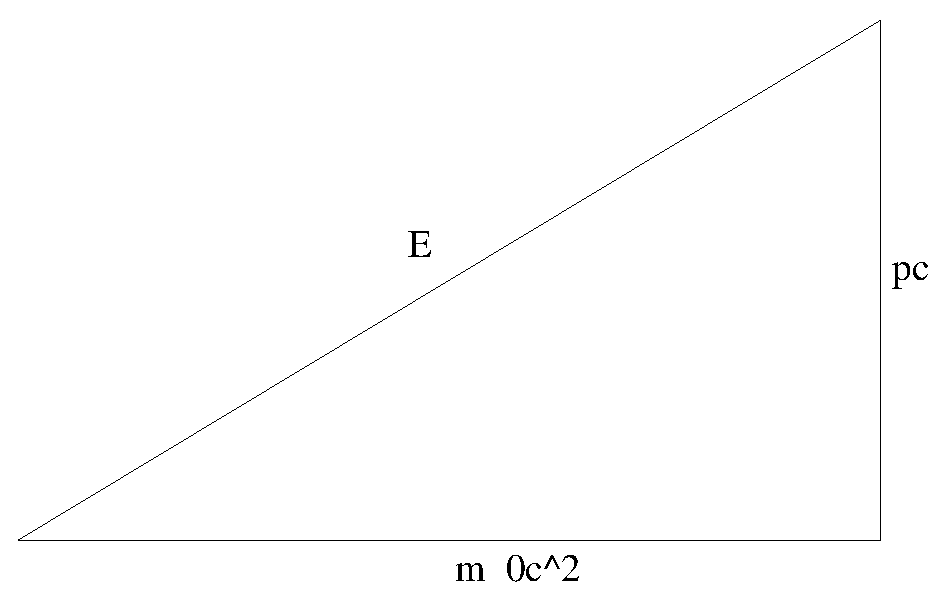
\includegraphics[scale=0.4]{immagini/fisica1/Trg_rel}
\end{figure}

\section{Elettronvolt\index{elettronvolt}}
La carica dell'elettrone vale circa $\si{1.6E-19}{\coulomb}$. $\si{1}{\electronvolt}$ è quell'energia che acquista un elettrone accelerato da una ddp di $\si{1}{\volt}$
\[
E=qV\qquad \electronvolt=q_e(\si{1}{\volt})=\si{1.6E-19}{\joule}
\]
Molto usati sono i multipli: \kilo\electronvolt (chev), \mega\electronvolt (mev), \giga\electronvolt (gev), \tera\electronvolt (tev), \peta\electronvolt (pev).

Anche le masse e le quantità di moto si possono esprimere in \electronvolt, combinando opportunamente con $c$.
\[E=mc^2\]
\[\si{1}{\kilo\gram},c^2=\si{1}{\kilo\gram}(\si{3E8}{\metre\per\second})=\si{9E16}{\joule}=\si{5.62E35}{\electronvolt} \]
\[\si{1}{\electronvolt}/c^2=\si{1.78E-36}{\kilogram} \]
\begin{Es}[decadimento particella strana]
Si vuole determinare il momento finale dei prodotti del decadimento della $K_0$:
\begin{figure}[htbp]
   \centering
   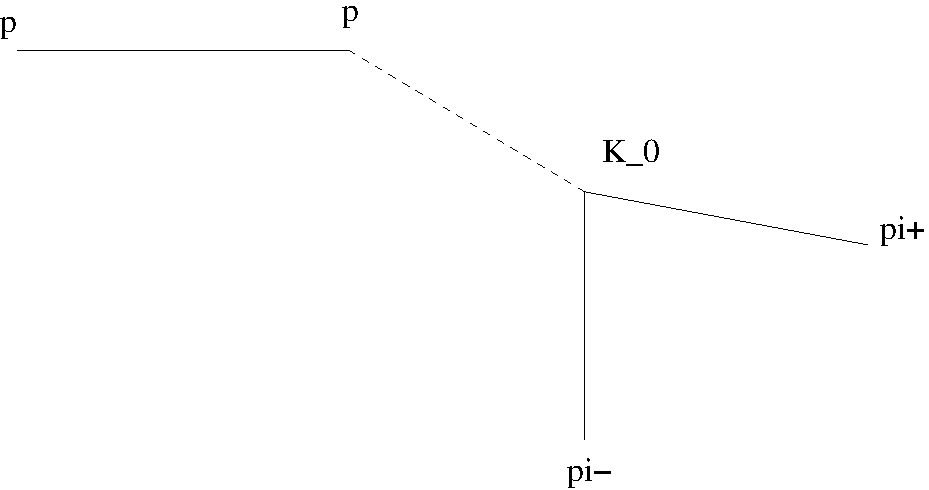
\includegraphics[scale=0.5]{immagini/fisica1/dec_strano}
   \caption{Un protone urta un protone fisso, si genera un $K_0$ che non è rilevabile in quanto neutro, dopo $\tau$ decade nei mesoni.}
   \label{}
\end{figure}
\[K_0\rightarrow \pi^+\,\pi^-\]
\[m_0^{K_0}=\si[per=slash,eVcorrb=0.4ex]{500}{\mega\eVperc\squared} \qquad m_0^{\pi^+}=\si{140}{\mega\eVperc\squared}\]
\[\tau_{K_0}=\si{0.9E-10}{\second} \]
Nel sistema di $K_0$ l'impulso dei mesoni è:
\begin{figure}[htbp]
   \centering
   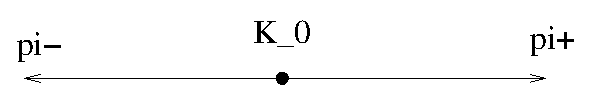
\includegraphics[scale=0.5]{immagini/fisica1/dec_strano2}
\end{figure}
\[
\ve p_0=0\quad \Rightarrow \quad \ve p_f=0 = \ve p_{\pi^+}+\ve p_{\pi^-}
\]
\[
m_0^{\pi^+}=m_0^{\pi^-}=m_0^{\pi}\qquad p_{\pi^+}=p_{\pi^-}=p_{\pi}\quad E_0=E_f
\]

\[E_0=m_0^{K_0}c^2=E_f=\sqrt{(m_0^{\pi^+}c^2)^2+p_{\pi^+}^2c^2}+\sqrt{(m_0^{\pi^-}c^2)^2+p_{\pi^-}^2c^2}=\]
\[=2\sqrt{(m_0^\pi c^2)^2+p_{\pi}^2c^2}\]
\[(m_0^{K_0})^2c^4=4(m_0^\pi c^2)^2+4p_{\pi}^2c^2\]
\[p_\pi^2=\frac{(m_0^{K_0})^2c^4-4(m_0^{\pi})^2c^4}{4c^2}=\frac{(m_0^K)^2c^2}{4}-(m_0^\pi)^2c^2\]
\[p_\pi=c\sqrt{\frac{(m_0^K)^2}{4}-(m_0^\pi)^2}\]
\end{Es}
\section{Forza e accelerazione\index{forza!relativistica}\index{accelerazione!relativistica}}
Newton: $\ve F=m\ve a$
\[\ud K=\ve F\cdot\ve{ \ud s}\]
\[E=mc^2=K+m_0c^2\qquad \ud m=\frac{1}{c^2}\ud K=\frac{1}{c^2}\ve F\cdot \ud \ve s\]
partiamo da quantità che abbiamo già ben definito in relatività: $p$ e $t$
\[\ve F=\frac{\ud \ve p}{\ud t}=\frac{\ud}{\ud t}(m\ve v)=\frac{\ud m}{\ud t}\ve v+m\frac{\ud \ve v}{\ud t}=\frac{1}{c^2}\ve F\frac{\ud \ve s}{\ud t}\ve v+m\ve a=\frac{1}{c^2}(\ve F\ve v)\ve v+m\ve a\]
La direzione di $\ve F$ e di $\ve a$ non è la stessa (!)
\subsection{Casi Particolari}
\subsubsection{$\ve F // \ve v$}
\[F=\frac{1}{c^2}Fv^2+ma\]
\[F=\frac{ma}{1-\beta^2}=\frac{m_0}{1-\beta^2}(1-\beta^2)^{-1/2}a=\underbrace{\frac{m_0}{(1-\beta^2)^{3/2}}}_{\text{massa longitudinale}}a=m_{//}a\]\index{massa!longitudinale}
\subsubsection{$\ve F\bot\ve v$}
\[\ve F=m\ve a=\underbrace{\frac{m_0}{\sqrt{1-\beta^2}}}_\text{massa trasversa}\ve a=m_\perp \ve a\]\index{massa!trasversa}
\begin{Es}[elettrone in campo magnetico]
\[\ve F=q\ve v\times\ve B\]
Campo magnetico ortogonale alla velocità\footnote{per una trattazione più completa vedi \ref{es_Larmor} a pag.\@\pageref{es_Larmor}}
\[F=qvB=m_\bot\frac{v^2}{r}\]
\[r=\frac{m_\bot v}{qB}=\frac{p}{qB}\]
\[\ve F\bot \ve v\Rightarrow L=0\Rightarrow v=\const\Rightarrow p=\const\Rightarrow r=\const\]
\[B=\si{2}{\weber\per\meter\squared} \qquad K=\si{10}{\mega\electronvolt} \]
\[r=\si{1.8}{\centi\meter} \quad\text{Relativistico}\]
\[r=\si{0.5}{\centi\meter} \quad\text{Classico}\]
\end{Es}


\pagebreak
\section{Spazio di Minkowski\index{Minkowski}\index{spazio!di Minkowski}}
\begin{wrapfigure}[10]{r}{5.6cm}
   \centering
   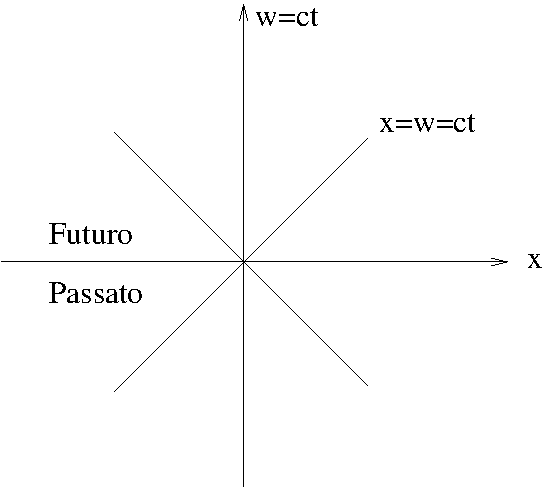
\includegraphics[scale=0.5]{immagini/fisica1/Mink1}
\end{wrapfigure}
Lo spazio di Minkowski è utile per dare un significato geometrico alla relatività speciale.
Per comodità grafiche consideriamo solo una coordinata spaziale e una temporale. Sull'asse delle ascisse rappresentiamo $x$ e sull'asse delle ordinate il tempo moltiplicato per $c$, che lo rende uno spazio.
La bisettrice dei quadranti è la linea di universo della luce, essa rappresenta il cammino di un raggio luminoso.
\[\frac{\ud w}{\ud x}=\frac{\ud(ct)}{\ud x}=c\frac{1}{\frac{\ud x}{\ud t}}=\frac{c}{v}>1\]
Quindi la traiettoria di ogni punto massivo nel piano di Minkowski deve avere tangente in ogni punto maggiore di uno, altrimenti andrebbe più veloce della luce.
Creiamo un nuovo sistema di riferimento inerziale.
\[\left\{\begin{array}{l}
x'=\frac{x-ut}{\sqrt{1-\beta^2}}\\
t'=\frac{t-\frac{\beta}{c}x}{\sqrt{1-\beta^2}}\\
\end{array}\right.\qquad
\left\{\begin{array}{l}
x'=\frac{x-\beta w}{\sqrt{1-\beta^2}}\\
w'=\frac{w-\beta x}{\sqrt{1-\beta^2}}\\
\end{array}\right.\]
\begin{wrapfigure}[14]{r}{6cm}
   \centering
   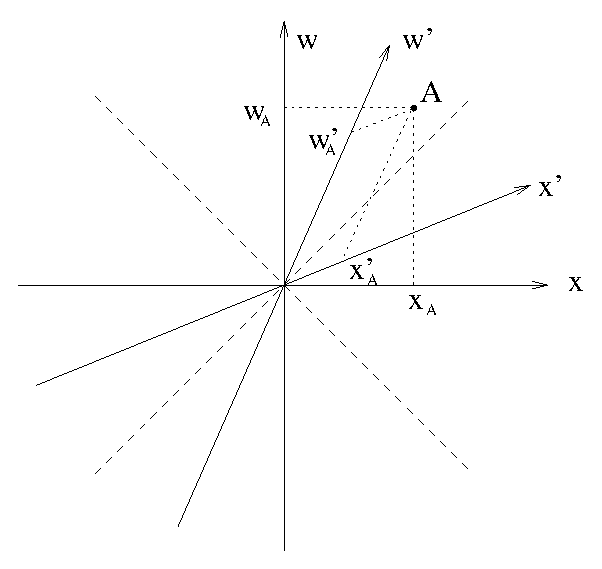
\includegraphics[scale=0.6]{immagini/fisica1/Mink2}
\end{wrapfigure}

\[w'=ct'=\frac{ct-\beta x}{\sqrt{1-\beta^2}}\]
asse $x'$: $w'=0$, cioè
\[w=\beta x\]
asse $w'$: $x'=0$, cioè
\[w=\frac{x}{\beta}\]

Più $\beta$ tende a $1$ e più i due assi del nuovo sistema di riferimento tendono alla bisettrice del primo--terzo quadrante.


\subsection{Dilatazione dei tempi\index{dilatazione dei tempi}}
\begin{figure}[htbp]
   \centering
   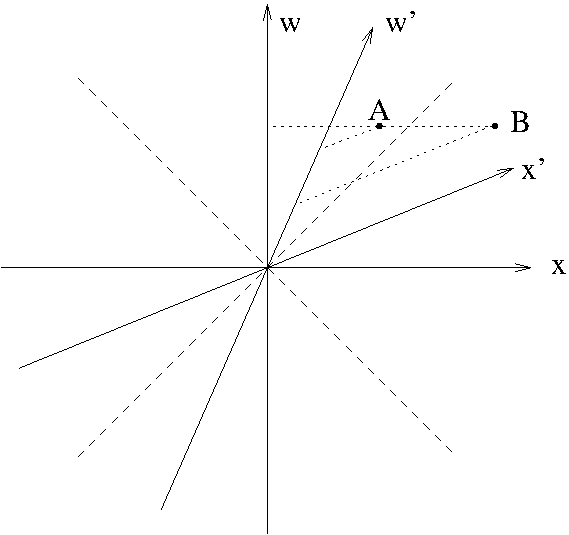
\includegraphics[scale=0.6]{immagini/fisica1/Mink3}
\end{figure}
$A$ e $B$ sono due eventi simultanei per $OXY$, ma non lo sono per $OX'Y'$. Analogamente si dimostra la contrazione delle lunghezze.

\subsection{Curve di calibrazione\index{curve! di calibrazione}}
\begin{figure}[htbp]
   \centering
   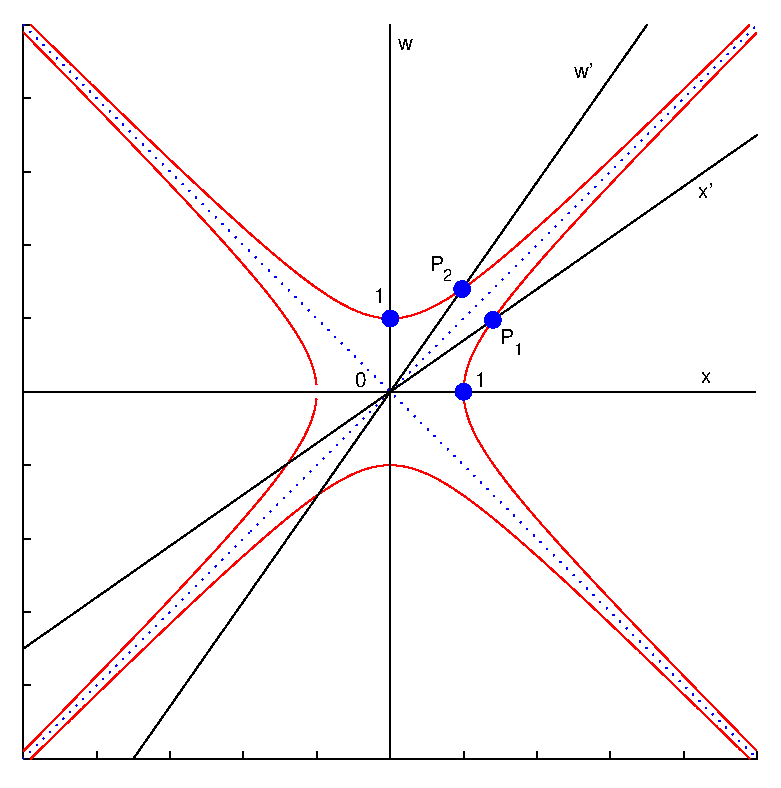
\includegraphics[scale=0.7]{immagini/fisica1/Minkowski_calibrazione}
   \caption{Curve di calibrazione.}
\end{figure}
\[\left\{\begin{array}{l}
w^2-x^2=1\\
x^2-w^2=1\end{array}\right.\]

\[P_1\left\{\begin{array}{l}
x^2-w^2=1\\
w'=0\\
\end{array}\right.\qquad \left\{\begin{array}{l}
x^2(1-\beta^2)=1\\
x=\frac{1}{\sqrt{1-\beta^2}}\end{array}\right.\]
\[x'=\dfrac{\dfrac{1}{\sqrt{1-\beta^2}}-\beta w}{\sqrt{1-\beta^2}}=\dfrac{\dfrac{1}{\sqrt{1-\beta^2}}-\beta^2 x}{\sqrt{1-\beta^2}}=\dfrac{\dfrac{1}{\sqrt{1-\beta^2}}-\dfrac{\beta^2}{\sqrt{1-\beta^2}}}{\sqrt{1-\beta^2}}=1\]
\[P_1(1,0)\qquad P_2(0,1)\]
\[\media{OP_1}>\media{01}\qquad\media{OP_2}>\media{01}\]


\section{Dubbi di Einstein}
Einstein si interrogava di come le forze potessero propagarsi, in particolare quella gravitazionale. Se il Sole scomparisse per Newton la Terra istantaneamente partirebbe per la tangente. Per Einstein ciò è impossibile, perché nulla, nemmeno la forza gravitazionale, o l'informazione ``il Sole non c'è più'', può viaggiare più veloce della luce. Con la generale si risolve il problema, la massa incurva lo spazio.

\index{relatività!speciale|)}
\chapter{Onde\index{onde}}
\minitoc
Le onde sono un moto che trasporta energia, mentre generano uno spostamento netto di materia nullo. Le onde\index{onda!meccanica} meccaniche sono quelle che hanno bisogno di un mezzo elastico per propagarsi, le onde elettromagnetiche\index{onda!elettromagnetica} si propagano anche nel vuoto. Le onde\index{onda!trasversale} trasversali sono quelle in cui la direzione di propagazione dell'onda è ortogonale al moto delle particelle. Le onde\index{onda!longitudinale} longitudinale sono quelle in cui le vibrazioni sono parallele alla velocità dell'onda. Le onde possono essere monodimensionali\index{onda!monodimensionale} (corda ideale vibrante), bidimensionali\index{onda!bidimensionale} (sasso nell'acqua), tridimensionali\index{onda!tridimensionale} (suono). Di solito quando si parla di onde si parla di treno d'onde\index{treno d'onde} periodico, il caso più semplice è l'onda armonica\index{onda!armonica} in cui tutte le particelle subiscono un moto armonico semplice. Per le onde trasversali si parla anche di polarizzazione\index{polarizzazione}, cioè l'orientamento del piano di vibrazione, che può essere costante (onda polarizzata) o meno.

Se mandiamo due impulsi in un mezzo elastico:
\begin{figure}[htbp]
   \centering
   \includegraphics[scale=0.5]{immagini/fisica1/Onda1}
\end{figure}
\[f(x)=f(x')=f(x-vt)\]
questo perché la forma d'onda non cambia. Questa è un'onda progressiva\index{onda!progressiva}, cioè un'onda che si propaga nel verso positivo delle $x$, se fosse al contrario sarebbe un'onda regressiva\index{onda!regressiva} e sarebbe
\[f(x)=f(x+vt)\]
\section{Onde sinusoidali}
Caso onda progressiva: $y(x,t)=f(x-vt)$
al tempo zero:
\[y(x,0)=f(x)=y_m\sin\left(\frac{2\pi}{\lambda} x\right)\]
\[\lambda=vT\]
\[y(x,t)=f(x-vt)=y_m\sin\left[2\pi\left(\frac{x}{\lambda}-\frac{t}{T}\right)\right]=y_m\sin\left(kx-\omega t\right)\]
\[k=\frac{2\pi}{\lambda}\qquad \omega=\frac{2\pi}{T}=2\pi\nu\]
$k$ numero d'onda, $\omega$ pulsazione. Considerando anche la fase $\varphi$:
\[y(x,t)=y_m\sin\left(kx-\omega t+\varphi\right)\]
\section{Corda Tesa\index{onda!su corda tesa}\index{corda tesa}}
\begin{figure}[htbp]
   \centering
   \includegraphics[scale=0.4]{immagini/fisica1/Onde_Corda}
\end{figure}
Trascuriamo il peso. Sull'elemento infinitesimo $\ud x$ agiscono due tensioni:
\[\ve T'+\ve T=\ud m \ve a\]
\[\left\{\begin{array}{l}
T'\cos\alpha'-T\cos\alpha=\ud m a_x=0\\
T'\sin\alpha'-T\sin\alpha=\ud m a_y\\
\end{array}\right.\]
Per deformazioni piccole usiamo il primo sviluppo di Taylor:
\[\cos \alpha=1+\ldots\qquad \sin \alpha=\alpha+\ldots\]
\[\left\{\begin{array}{l}
T'=T\\
T'\alpha'-T\alpha=\ud m a_y=\ud m a\\
\end{array}\right.\]
Ma il primo sviluppo di Taylor del seno è uguale a quello della tangente:
\[T\tan\alpha'-T\tan\alpha=\ud m a\]
Ma la tangente è la derivata delle $y$ nelle $x$:
\[T\left.\frac{\partial y}{\partial x}\right |_{x+\ud x}\!\!\!\!\!\!\!\!\!\!-T\left.\frac{\partial y}{\partial x}\right|_{x}=\ud m\frac{\partial^2 y}{\partial t^2}\]
\[T\left.\frac{\partial^2 y}{\partial x^2}\right|_x\ud x=\frac{\partial^2 y}{\partial t^2}\ud m\]
Chiamiamo $\rho$ la densità lineare:
\[\rho=\frac{\ud m}{\ud s}\qquad \ud m=\rho s\qquad \ud s\cos\alpha=\ud x\qquad\ud m=\rho\ud x\]
\[T\left.\frac{\partial^2 y}{\partial x^2}\right|_x\ud x=\rho\frac{\partial^2 y}{\partial t^2}\ud x\]
\[\frac{\partial^2 y}{\partial x^2}=\frac{\rho}{T}\frac{\partial^2 y}{\partial t^2}\qquad\text{equazione di D'Alembert}\]

\parbox[]{\textwidth}{
\section{Equazione differenziale di un'onda\index{equazione!differenziale di un'onda}}
Nel caso progressivo:
\[y=f(x-vt)\qquad z=x-vt\]
\[\frac{\partial y}{\partial z}=\frac{\partial y}{\partial t}\frac{\partial t}{\partial z}=\frac{\partial y}{\partial t}\frac{1}{\frac{\partial z}{\partial t}}=-\frac{1}{v}\frac{\partial y}{\partial t}\]
\[\frac{\partial y}{\partial z}=\frac{\partial y}{\partial x}\frac{\partial x}{\partial z}=\frac{\partial y}{\partial x}\frac{1}{\frac{\partial z}{\partial x}}=\frac{\partial y}{\partial x}\]
}

\[\frac{\partial^2 y}{\partial z^2}=\frac{\partial}{\partial z}\left(\frac{\partial y}{\partial z}\right)\frac{\partial t}{\partial t}=\frac{\partial}{\partial t}\left(-\frac{1}{v}\frac{\partial y}{\partial t}\right)\frac{\partial t}{\partial z}=\frac{1}{-v}\left(\frac{\partial^2 y}{\partial t^2}\right)\frac{1}{-v}=\frac{1}{v^2}\frac{\partial^2 y}{\partial t^2}\]
\[\frac{\partial^2 y}{\partial z^2}=\frac{\partial}{\partial z}\left(\frac{\partial y}{\partial z}\right)=\frac{\partial}{\partial z}\left(\frac{\partial y}{\partial x}\right)\frac{\partial x}{\partial x}=\frac{\partial}{\partial x}\left(\frac{\partial y}{\partial x}\right)\frac{\partial x}{\partial z}=\frac{\partial^2 y}{\partial x^2}\]

\begin{equation}
\frac{\partial^2 y}{\partial x^2}=\frac{1}{v^2}\frac{\partial^2 y}{\partial t^2}
\end{equation}

Nel caso della corda tesa $v=\sqrt{\frac{T}{\rho}}$. Nella velocità ci sono sempre due termini, uno di elasticità del mezzo (in questo caso $T$) e uno di inerzia (in questo caso $\rho$).

Nel caso di onda regressiva l'equazione differenziale è uguale, anche nei segni.
\section{Velocità e accelerazione trasversale}
\[u_y(x,t)=\frac{\partial y}{\partial t}=\frac{\partial}{\partial t}\left[y_m\sin\left(kx-\omega t\right)\right]=-y_m\omega\cos\left(kx-\omega t\right)\]
\[a_y(x,t)=\frac{\partial u_y}{\partial t}=-y_m\omega^2\sin\left(kx-\omega t\right)=-\omega^2 y\]
\section{Principio di sovrapposizione\index{principio!di sovrapposizione}}
\begin{Pri}[sovrapposizione]
In un mezzo in cui due onde si sovrappongono, la perturbazione è la somma delle due onde.
\end{Pri}
\subsection{Interferenza\index{interferenza}}
\begin{figure}[htbp]
   \centering
   \includegraphics[scale=0.5]{immagini/fisica1/interferenza_distruttiva}
   \caption{Interferenza distruttiva\index{interferenza!distruttiva}.}
\end{figure}
L'interferenza è la sovrapposizione di due onde sinusoidali. Prendiamo due onde progressive, sinusoidali, con stessa ampiezza e frequenza, ma con diversa fase. La differenza di fase è la costante di fase.
\[y_1=y_m\sin(kx-\omega t)\qquad y_2=y_m\sin(kx-\omega t+\varphi)\]
\begin{align*}
y_1+y_2&=y_m\left[\sin\left(kx-\omega t\right)+\sin\left(kx-\omega t+\phi\right)\right]\\
&=y_m\left[2\cos\frac{\varphi}{2}\sin\left(kx-\omega t+\frac{\varphi}{2}\right)\right]\\
&=\left(2y_m\cos\frac{\varphi}{2}\right)\sin\left(kx-\omega t+\frac{\varphi}{2}\right)
\end{align*}
L'ampiezza delle onde non è più costante, ma è una funzione armonica. Si distinguono due casi particolari:
\begin{align*}
\varphi&=0+2k\pi&y_m&\rightarrow 2y_m&\text{Interferenza costruttiva}\\
\varphi&=\pi+2k\pi&y_m&\rightarrow 0&\text{Interferenza distruttiva}
\end{align*}
\section{Onde stazionarie\index{onda!stazionaria}}
Le onde stazionarie sono il frutto dell'interferenza di un'onda progressiva e una regressiva, tipicamente di un'onda con la sua riflessa.

\parbox[]{\textwidth}{
\[
y_1=y_m\sin\left(kx-\omega t\right)\qquad y_2=y_m\sin\left(kx+\omega t\right)
\]
\begin{align*}
y=&y_1+y_2=y_m\left[\sin\left(kx-\omega t\right)+\sin\left(kx+\omega t\right)\right]\\
=&2y_m\left[\sin\left(kx\right)\cos\left(\omega t\right)\right]
\end{align*}
}
La parte spaziale e quella temporale si separano. Se consideriamo con ampiezza $2y_m\sin\left(kx\right)$ allora ci sono dei punti dove il seno si annulla che non vibrano, sono i \index{nodi}nodi, mentre dove la vibrazione è massima ci sono i ventri\index{ventri}. Nodi:
\[\sin\left(kx\right)=0\qquad kx=0,\pi,\ldots\]
\[n\pi=kx\qquad k=\frac{2\pi}{\lambda}\qquad x=n\frac{\lambda}{2}\]
Le onde stazionarie non trasportano energia.
\begin{figure}[htbp]
   \centering
   \includegraphics[scale=0.5]{immagini/fisica1/stazionarie1}
   \caption{famiglia di onde stazionarie disegnate a intervalli costanti di tempo.}
   \includegraphics[scale=0.7]{immagini/fisica1/stazionarie2}
   \caption{Onde stazionarie in tre dimensioni.}
\end{figure}

\section{Effetto Doppler\index{effetto!Doppler}\index{Doppler}}
L'effetto Doppler si sviluppa quando la sorgente delle onde e l'osservatore sono in moto relativo.
Immaginando la sorgente che emette onde con velocità di propagazione $u$ e lunghezza d'onda $\lambda$ ferma e l'osservatore in allontanamento con velocità $v$ il numero di fronti d'onda che l'osservatore riceve nel tempo $t$ è:
\[N=\nu t=\nu_0t-\frac{vt}{\lambda}\]
\begin{subequations}
\begin{equation}
\nu=\nu_0+\frac{v}{\lambda}=\nu_0-\frac{v}{u}\nu_0=\nu_0\left(1-\frac{v}{u}\right)
\end{equation}
Nel caso inverso nel quale sia la sorgente a muoversi con velocità $v$ bisogna scambiare $\nu$ con $\nu_0$:
\begin{equation}
\nu=\nu_0\frac{u}{u-v}
\end{equation}
\end{subequations}
notiamo che non c'è simmetria, cioè se consideriamo sorgente ferma e osservatore in moto con velocità $v$ non otteniamo lo stesso risultato di osservatore fermo e sorgente in moto con velocità $-v$. Questo perché esiste un sistema privilegiato che è il mezzo in cui si propaga l'onda. Questo non è vero per le onde elettromagnetiche.
\subsection{Effetto Doppler relativistico\index{effetto!Doppler!relativistico}}
Consideriamo l'ultimo caso trattato in funzione del periodo anziché della frequenza nel caso di onde luminose:
\[
T=T_0'\left(1-\frac{v}{c}\right)
\]
$T_0'$ è il periodo proprio della sorgente misurato da un osservatore che si muove con la sorgente alla velocità $v$, quindi dall'osservatore fermo esso viene percepito come:
\begin{subequations}
\begin{equation}
T_0=\frac{T_0'+\frac{\beta}{c}x'}{\sqrt{1-\beta^2}}
\end{equation}
Se consideriamo la sorgente come origine del sistema in moto allora $x'=0$:
\begin{equation}
T=\frac{T_0\left(1-\beta\right)}{\sqrt{1-\beta^2}}
\end{equation}
\end{subequations}
\section{Suono\index{suono}}
Il suono è un'onda longitudinale che si propaga di solito nell'aria provocando zone con maggiore pressione e zone con minore pressione e quindi zone con maggior densità e zone di rarefazione. Il suono percepito dall'uomo è quello che ha frequenza $\SIrange[tophrase=dots]{20}{20000}{\hertz}$. Sotto ci sono gli infrasuoni, sopra gli ultrasuoni. La velocità del suono è\index{velocità!del suono}:
\begin{equation}
v=\sqrt{\frac{B}{\rho}}
\end{equation}
$B$ è il coefficiente di comprimibilità definito come:
\begin{equation}
B=\frac{-\Delta p}{\Delta V/V}
\end{equation}
Se approssimiamo il comportamento dell'aria ad un gas adiabatico, supponendo quindi che il suono si propaghi più veloce del calore si ha:
\[PV^\gamma=\const\qquad \ud PV^\gamma+P\gamma V^{\gamma-1}\ud V=0\]
\[\frac{\ud P}{\ud V/V}=-\gamma P\qquad v=\sqrt{\frac{\gamma P}{\rho}}=\si{330}{\metre\per\second} \]
\section{Grandezze caratteristiche}
\begin{description}
\item[intensità\index{intensità!del suono} del suono] $I=\text{Energia}/\text{tempo superficie}$\\
\item[soglia\index{soglia!di udibilità} di udibilità] $I_0=\si{1E-12}{\watt\per\meter\squared}$\\
\item[altezza\index{altezza!del suono} del suono]la frequenza\\
\item[timbro \index{timbro}del suono] è la forma d'onda, cioè la composizione in armoniche dello sviluppo di Fourier\\
\item[sensazione\index{sensazione sonora} sonora] non è lineare $10\log_{10} I/I_0$ e si misura in decibel \si{}{\deci\bel}\\
\item[soglia del \index{soglia!del dolore}dolore] $\si{120}{\deci\bel}$\\
\end{description}




























%\chapter{Ottica geometrica\index{ottica!geometrica|(}}
%L'ottica geometria è il modo di studiare l'ottica più antico. Nel '600 non si aveva %chiaro cosa fosse la luce e veniva descritta attraverso i raggi.
%
%\section{Onde}
%\begin{figure}[htbp]
%\includegraphics[scale=0.3]{immagini/fisica1/fronti_donda}
%\caption{Fronti d'onda circolare e raggi.}
%\end{figure}
%\begin{figure}[htbp]
%\includegraphics[scale=0.4]{immagini/fisica1/frontilontani}
%\caption{Fronti d'onda circolare a grande distanza sono considerati piani.}
%\end{figure}
%Ogni onda è descritta dai fronti d'onda\index{fronti!d'onda}, che corrispondono alle %creste e ai seni dell'onda. I raggi \index{raggi d'onda}sono segmenti orientati, %perpendicolari ai fronti d'onda, uscenti dalla sorgente. Le onde si dividono in sferiche, %circolari, piane, \ldots a seconda della geometria. Spesso a grandi distanze dalla %sorgente possono essere descritte come onde piane.
%
%I corpi colpiti da radiazione elettromagnetica in parte la riflettono, in parte la %assorbono e in parte la trasmettono. I corpi opachi assorbono molto, cioè trasformano la %luce in qualcos'altro (calore). I corpi trasparenti trasmettono molta luce. Bisogna %indicare rispetto a che radiazione i corpi sono trasparenti o opachi, per esempio il %vetro, trasparente alla luce visibile, è opaco agli UV.
%
%Quasi tutti i corpi opachi (non le superfici riflettenti) diffondono la luce in tutte le %direzioni, si parla di riflessione diffusa, cioè riflettono la luce in tutte le direzioni.
%
%\begin{Pri}[Fermat]
%il percorso della luce è tale che risulti stazionario, cioè è un minimo o un massimo.
%\end{Pri}
%
%\section{Riflessione\index{riflessione}}
%\subsection{Specchio piano\index{specchio!piano}}
%Come negli urti il raggio riflesso e quello incidente stanno nello stesso piano %individuato con la normale; l'angolo di incidenza è uguale a quello di riflessione.
%\begin{figure}[htbp]
%\includegraphics[scale=0.5]{immagini/fisica1/riflessione}
%\end{figure}
%\subsection{Elissoide}
%\[\overline{F_1P}=\overline{F_2P}\]
%\subsection{Specchi sferici\index{specchio!sferico}}
%Angoli piccoli, piccole aperture.
%Specchio concavo $R>0$, specchio convesso $R<0$.
%Immagine reale $q>0$, immagine virtuale $q<0$
%\[\frac{1}{p}+\frac{1}{q}=\frac{1}{f}\]
%Quindi se i raggi sono paralleli:
%\[p\rightarrow{\infty}\Rightarrow p\rightarrow f=\frac{R}{2}\]
%\section{Rifrazione\index{rifrazione}}
%La rifrazione avviene quando cambia il mezzo:
%\[\frac{\sin i}{\sin r}=n_{12}=\frac{n_2}{n_1}\]
%\[n_{12}=\text{indice di rifrazione relativo ai due mezzi}\]
%\[n_1=\text{indice di rifrazione assoluto del primo mezzo (rispetto al vuoto)}>1\]
%l percorso non risulta il più corto, ma è il più breve (è un minimo):
%\[t_A^B=t_1+t_2=\frac{AP}{v_1}+\frac{PB}{v_2}=\frac{n_1}{c}AP+\frac{n_2}{c}PB=\frac{1}{c}(%n_1AP+n_2PB)\]
%
%\subsection{Lenti sottili\index{lenti!sottili}}
%\[\frac{1}{p}+\frac{1}{q}=\frac{1}{f}=(n-1)\left(\frac{1}{R_1}-\frac{1}{R_2}\right)\]
%\index{ottica!geometrica|)}
